\documentclass[journal]{IEEEtran}

\usepackage{cite}
\usepackage{amsmath,amssymb,amsfonts}
\usepackage{graphicx}
\usepackage{textcomp}
\usepackage{subcaption}
\usepackage{booktabs}
\usepackage{multirow}
\usepackage{microtype}
\usepackage{caption}
\usepackage{balance}
\usepackage{algorithm}
\usepackage{algpseudocode}
\usepackage{siunitx}
\captionsetup{font=small,labelfont=bf}

\graphicspath{{framework/}{representation/}{AW-DPCNN/}{MSCA-VGG16/}{Fused images/}{equipment/}{confusion_matrix/}{tsne/}{tsne_cwru/}{raw_tsne/}{tsne_models/}{figures/}}

\hyphenation{op-tical net-works semi-conduc-tor IEEE-Xplore}

\begin{document}

% \title{AW-DPCNN Based Multi-Representation Supervised Learning for Mechanical Signal Fault Diagnosis}
% \title{AW-DPCNN: Adaptive-Weighted Dual-PCNN Fusion of Time-Frequency Representations for Non-Stationary Fault Diagnosis}
\title{Adaptive Dual-Branch PCNN Multi-Representation Fusion Network for Non-Stationary Signal Fault Diagnosis}

\author{Chen Yang, Zonglong Bai, Zhiyuan Xie, Chenggang Liu, Junyan Zhang and Yihe Guo}

\markboth{IEEE Transactions on Instrumentation and Measurement}
{Author~\MakeLowercase{\textit{et al.}}: AW-DPCNN Based Multi-Representation Supervised Learning for Mechanical Signal Fault Diagnosis}

\maketitle

\begin{abstract}
Non-stationary vibration signals from rotating machinery pose significant challenges for intelligent fault diagnosis, as conventional single-representation methods often fail to capture the full spectrum of discriminative fault information. This paper presents an Adaptive Weighted Dual-branch Pulse-Coupled Neural Network (AW-DPCNN) for multi-representation fusion, coupled with a Multi-Scale Channel Attention enhanced VGG16 (MSCA-VGG16) classifier, to address the limitations of existing approaches in fusing heterogeneous time--frequency and temporal-encoded representations. The AW-DPCNN introduces three key mechanisms: dual-channel external stimuli that independently process time--frequency representations and Gramian Angular Difference Field (GADF) encodings through representation-specific convolutional kernels; a contrast-guided adaptive weighting scheme that dynamically regulates the relative contribution of each representation based on local saliency; and iterative pulse-coupled dynamics that propagate and reinforce structurally consistent features while suppressing spurious activations. The fused representations are then classified by MSCA-VGG16, which integrates multi-scale convolution for capturing fault patterns across different temporal and spectral granularities, squeeze-and-excitation channel attention for dynamic frequency-band recalibration, and a compact discriminative embedding head for enhanced inter-class separation. Extensive experiments on the Case Western Reserve University (CWRU) bearing dataset demonstrate that AW-DPCNN fusion consistently outperforms single-representation baselines and naive concatenation strategies. The full AW-DPCNN + MSCA-VGG16 pipeline achieves 99.19\% accuracy on the 12 kHz drive-end benchmark, with strong generalization to fan-end sensor data (95.33\%) and cross-sampling-rate scenarios (94.81\% at 48 kHz). Comprehensive ablation studies, representation comparisons across twelve time--frequency and temporal encoding combinations, noise robustness evaluations, and hyperparameter sensitivity analyses collectively validate the effectiveness, robustness, and generalizability of the proposed framework for non-stationary mechanical signal fault diagnosis.
\end{abstract}

\begin{IEEEkeywords}
Fault diagnosis, Gramian angular difference field (GADF), multi-representation fusion, pulse coupled neural network (PCNN), rotating machinery, short-time Fourier transform (STFT), time--frequency analysis.
\end{IEEEkeywords}

\section{Introduction}
\IEEEPARstart{R}{otating} machinery, including bearings, gears, and shafts, constitutes the core of modern industrial systems. Unexpected failures of these critical components can lead to catastrophic breakdowns, substantial economic losses, and severe safety hazards~\cite{alonso-gonzalezBearingFaultDiagnosis2023}. Consequently, reliable and intelligent fault diagnosis techniques have become indispensable for condition-based maintenance and operational safety assurance~\cite{7033433}. Among various diagnostic modalities, vibration-based monitoring has received the most extensive research attention due to its rich fault-related information content, non-intrusive sensor deployment, and well-established physical understanding of fault-induced vibration signatures~\cite{5352306}.

Despite the practical success of vibration-based diagnosis, the non-stationary nature of real-world machinery signals remains a fundamental challenge. Under variable speed, fluctuating load, and time-varying operating conditions, vibration signals exhibit pronounced non-stationary characteristics — their spectral content and statistical properties evolve over time in complex ways that cannot be adequately captured by conventional stationary signal processing techniques~\cite{4717246}. Single time-domain or frequency-domain representations each capture only partial aspects of these rich signals: time-domain features may overlook critical spectral information, while frequency-domain representations discard temporal evolution patterns that are essential for distinguishing transient fault events from steady-state operating conditions~\cite{zhangFaultDiagnosisRecognition2024}.

To address the limitations of single-representation approaches, researchers have explored complementary representation strategies. Time--frequency representations such as the Short-Time Fourier Transform (STFT) spectrogram, Mel spectrogram, and continuous wavelet transform (CWT) scalogram provide joint time--frequency energy distributions that reveal how spectral content evolves temporally~\cite{10091539},~\cite{9760386}. In parallel, temporal encoding methods such as the Gramian Angular Field (GAF), Markov Transition Field (MTF), and Recurrence Plot (RP) transform one-dimensional time series into two-dimensional images by encoding pairwise temporal relationships, thereby preserving global temporal correlation structures that time--frequency methods may not explicitly capture~\cite{11048665},~\cite{10114345}. However, most existing studies adopt a single representation for downstream classification, and the complementary nature of time--frequency and temporal-encoded representations remains largely underexploited.

Multi-representation fusion offers a natural avenue to combine the strengths of heterogeneous representations, yet existing fusion strategies face critical limitations. Simple concatenation or pixel-wise averaging ignores the distinct statistical properties and structural characteristics of different representations, potentially introducing destructive interference rather than constructive complementarity~\cite{9408662}. Fixed-weight fusion schemes lack the adaptivity to emphasize discriminative representations while suppressing less informative ones on a per-sample or per-region basis. Furthermore, conventional deep learning classifiers, while powerful, often lack explicit architectural mechanisms to exploit the multi-scale and channel-wise characteristics of fused representations~\cite{9832890}.

To address these gaps, this paper proposes a two-stage framework comprising an Adaptive Weighted Dual-branch Pulse-Coupled Neural Network (AW-DPCNN) for multi-representation fusion, and a Multi-Scale Channel Attention enhanced VGG16 (MSCA-VGG16) classifier for robust fault identification. The main contributions are:

\begin{itemize}
\item An AW-DPCNN fusion mechanism is proposed to adaptively integrate time--frequency representations (STFT spectrogram) and temporal-encoded representations (GADF). The mechanism introduces contrast-guided adaptive weighting to dynamically regulate per-channel contributions, dual-channel external stimuli with representation-specific convolutional kernels, and iterative pulse-coupled dynamics for feature reinforcement.

\item An MSCA-VGG16 classification network is constructed to further exploit the complementary information encoded in the fused representations. The architecture integrates multi-scale convolution for capturing fault patterns at multiple temporal and spectral granularities, squeeze-and-excitation channel attention for dynamic frequency-band recalibration, and a compact embedding head for enhanced discriminability.

\item Extensive experiments on the CWRU bearing dataset — including backbone comparisons, comprehensive ablation studies, representation comparisons across twelve time--frequency and temporal encoding combinations, noise robustness evaluations at multiple SNR levels, and hyperparameter sensitivity analyses — systematically validate each component of the proposed framework.

\item Cross-sensor and cross-sampling-rate generalization is demonstrated on the CWRU 12 kHz fan-end and 48 kHz drive-end datasets, confirming the robustness and transferability of the proposed approach beyond the primary benchmark.

\end{itemize}

The remainder of this paper is organized as follows. Section~\ref{section2} reviews related work. Section~\ref{section3} presents the proposed AW-DPCNN fusion mechanism and MSCA-VGG16 classifier. Section~\ref{section4} describes the experimental setup and comprehensive performance evaluation. Finally, conclusions are drawn in Section~\ref{section5}.
\begin{figure*}[!htbp]
\centering
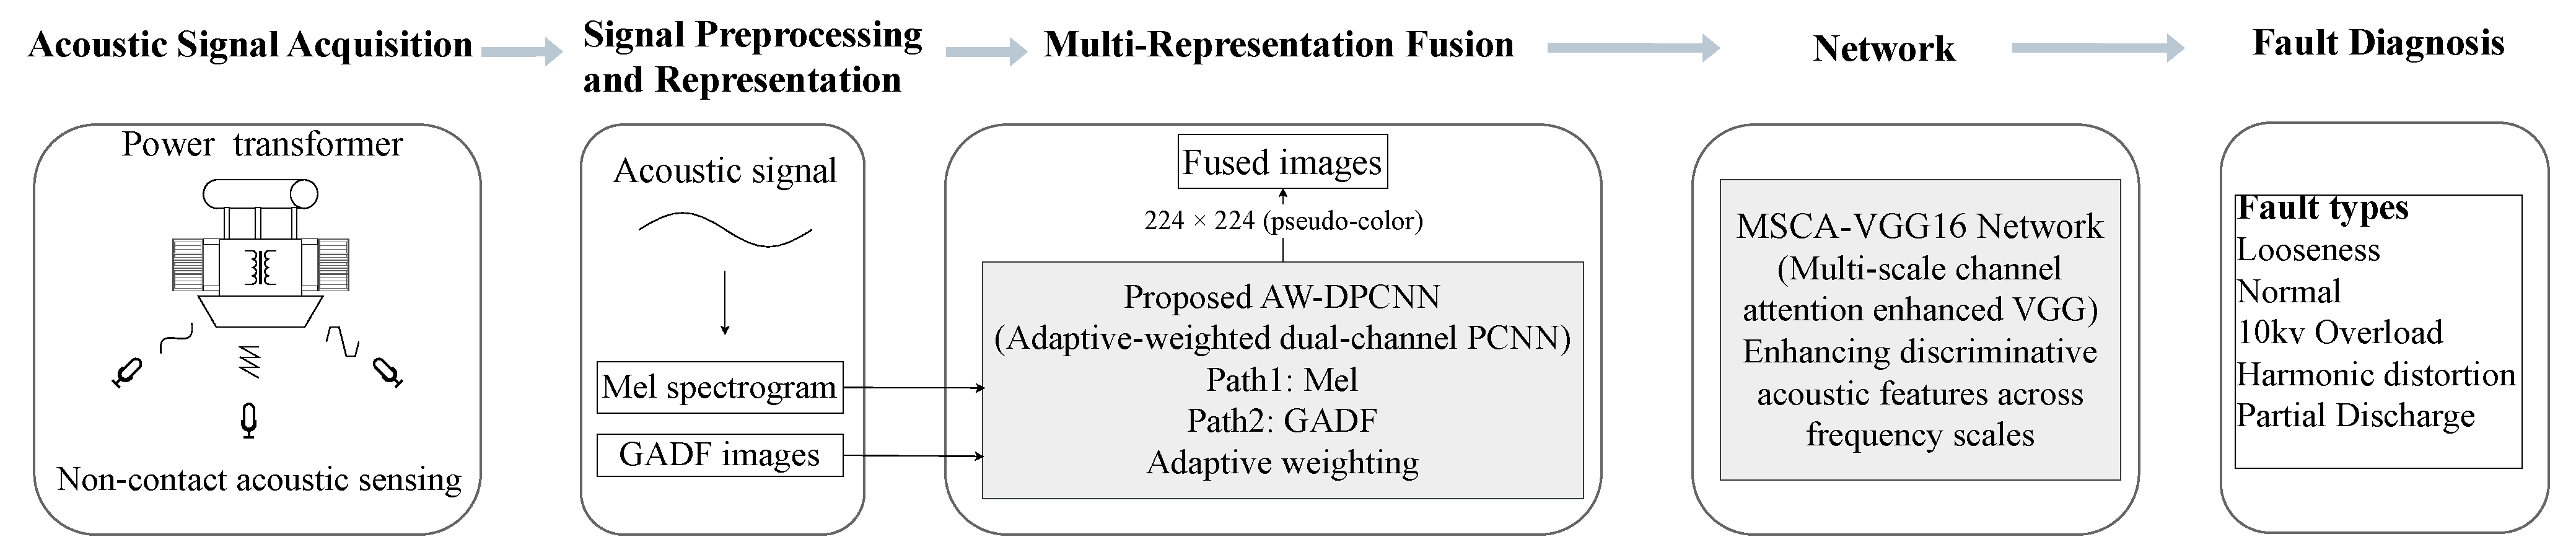
\includegraphics[width=\linewidth]{framework/framework}
\caption{Overall framework of the proposed bearing fault diagnosis method. The vibration signal is first converted into STFT spectrogram and GADF images. These heterogeneous representations are then adaptively fused through the proposed AW-DPCNN mechanism. Finally, the fused feature is fed into the MSCA-VGG16 network for fault classification.}
\label{framework}
\end{figure*}

\section{Related Work}
\label{section2}

\subsection{Signal Representations for Fault Diagnosis}

Vibration signals from rotating machinery are inherently non-stationary and exhibit complex frequency-dependent characteristics resulting from mechanical impacts, varying compliance, and speed fluctuations~\cite{5352306}. To extract discriminative fault-related information from such signals, various time--frequency representations have been explored. The STFT spectrogram provides a linear time--frequency decomposition with uniform frequency resolution, making it suitable for analyzing broadband impulsive fault signatures typical of bearing defects~\cite{7558591}. Mel spectrograms apply a perceptually motivated nonlinear frequency scaling that emphasizes low-frequency content, which can be beneficial for capturing harmonic structures associated with certain fault types~\cite{10091539}. The continuous wavelet transform (CWT) scalogram offers variable time--frequency resolution through multi-scale basis functions, enabling better localization of transient events~\cite{9760386}.

In parallel, temporal encoding methods transform one-dimensional time-series signals into two-dimensional images by encoding pairwise temporal correlations. The Gramian Angular Field (GAF) framework, encompassing both the Gramian Angular Summation Field (GASF) and Gramian Angular Difference Field (GADF), maps time series to polar coordinates and aggregates angular relationships through summation or difference operations~\cite{11048665},~\cite{10114345}. The Markov Transition Field (MTF) encodes temporal transition probabilities between discretized signal levels, capturing sequential dynamics~\cite{10281942}. The Recurrence Plot (RP) visualizes recurrent states in phase space, revealing underlying periodicities and nonlinear dynamics. These temporal encoding methods preserve global temporal correlation structures that time--frequency methods may not explicitly capture.

Despite these advances, individual time--frequency or temporal encoding representations each capture only partial aspects of vibration signals. Time--frequency representations primarily reflect local spectral energy distributions but may not fully describe global temporal correlations, while temporal encoding methods capture temporal dependencies but lack explicit frequency-domain information. This motivates the development of multi-representation fusion strategies that can jointly exploit complementary signal characteristics.

\subsection{PCNN and Multi-Modal Fusion}

Pulse-coupled neural networks (PCNNs) are neural models originally developed to simulate the synchronous firing behavior observed in the mammalian visual cortex \cite{4305279,6338347}. Unlike conventional convolutional neural networks, PCNNs employ a pulse-based activation mechanism in which neurons interact through local coupling and dynamic thresholds \cite{8742596}. Owing to these characteristics, PCNNs exhibit strong capability in preserving structural information while suppressing background interference, and have been widely applied in image segmentation, edge detection, and feature enhancement tasks \cite{9444355}, \cite{10848019}, \cite{8746999}. 

However, conventional PCNNs are typically driven by a single external stimulus, which limits their ability to effectively exploit complementary information from multiple representations. To address this limitation, dual-channel PCNN (DPCNN) architectures have been introduced to enable multi-representation fusion by incorporating multiple external stimuli within the neuronal feeding mechanism \cite{4344292}, \cite{10341267}. Through this mechanism, heterogeneous feature maps can be jointly processed, thereby facilitating the integration of information from different representations. Nevertheless, the fusion process in such architectures generally relies on fixed or predefined coupling strategies, making it difficult to adaptively regulate the relative contributions of different channels. As a result, the model may not effectively emphasize discriminative representations while suppressing less relevant ones, thereby limiting the effectiveness of multi-representation fusion.

\subsection{Deep Learning for Fault Diagnosis}

With the rapid advancement of deep learning techniques, a variety of neural network architectures have been applied to bearing fault identification and rotating machinery fault diagnosis, demonstrating superior automatic feature extraction capability compared with traditional handcrafted methods \cite{18184994}, \cite{7033433}. Early studies commonly adopted baseline convolutional neural networks as benchmark architectures for acoustic and vibration fault classification, verifying the feasibility of end-to-end feature learning for fault diagnosis tasks \cite{ahsanEnhancedFaultDiagnosis2025}. Subsequently, classical deep convolutional backbones, including AlexNet \cite{guNovelFaultDiagnosis2022}, VGG16 \cite{zhangFaultDiagnosisRecognition2024}, and ResNet18 \cite{maBearingFaultDiagnosis2024}, were introduced into intelligent fault diagnosis frameworks and achieved notable improvements in hierarchical feature representation and classification accuracy across machinery health monitoring applications \cite{11014495}, \cite{5352306}, \cite{4717246}. More recently, advanced architectures such as ConvNeXt-Tiny, which incorporate modernized convolutional design principles, have further enhanced representation learning capability and demonstrated competitive performance in fault diagnosis and image-based classification tasks \cite{zhangWaveConvNeXtEfficientPrecise2024}. In addition, publicly available benchmark datasets, such as the CWRU bearing fault dataset, have been extensively employed to evaluate the effectiveness and generalization ability of deep learning-based diagnostic models, serving as a standard reference in fault diagnosis research \cite{alonso-gonzalezBearingFaultDiagnosis2023}, \cite{zhangMachineLearningBased2021}.

Despite these advances, most existing deep learning approaches remain purely data-driven and primarily rely on a single representation. Consequently, their diagnostic performance strongly depends on large-scale labeled datasets and is vulnerable to degradation under noise interference, operating condition variations, and signal inconsistencies commonly encountered in practical industrial monitoring scenarios. Moreover, conventional deep learning models often lack explicit mechanisms to exploit complementary heterogeneous feature representations, limiting their robustness in complex fault diagnosis tasks.

\section{Methodology}
\label{section3}

\subsection{Overview}

The proposed framework comprises two sequential stages: multi-representation signal fusion and fused representation classification, as illustrated in Fig.~\ref{framework}. In the fusion stage, the raw vibration signal is first transformed into two complementary representations—the STFT spectrogram and the Gramian Angular Difference Field (GADF) image—to capture time--frequency energy distributions and global temporal correlation structures, respectively. These heterogeneous representations are then adaptively integrated through the proposed AW-DPCNN mechanism, which employs contrast-guided adaptive weighting and dual-channel pulse-coupled dynamics to produce a unified fused representation. In the classification stage, the fused representation is fed into the MSCA-VGG16 network, which incorporates multi-scale convolution and channel attention to enhance feature discrimination, followed by a compact embedding head for robust fault classification.

Formally, let $\boldsymbol{x} \in \mathbb{R}^{L}$ denote a raw vibration signal segment of length $L$. The signal is first mapped to two heterogeneous representations as

\begin{equation}
\boldsymbol{S}_{\mathrm{Mel}} = \mathcal{T}_{\mathrm{Mel}}(\boldsymbol{x}), \quad
\boldsymbol{S}_{\mathrm{GADF}} = \mathcal{T}_{\mathrm{GADF}}(\boldsymbol{x}),
\label{eq:pipeline_rep}
\end{equation}

where $\mathcal{T}_{\mathrm{Mel}}(\cdot)$ and $\mathcal{T}_{\mathrm{GADF}}(\cdot)$ denote the Mel spectrogram and GADF transformation operators, respectively, both producing pseudo-color RGB images of size $224 \times 224$. The two representations are then fused via the AW-DPCNN operator $\mathcal{F}_{\mathrm{AW}}(\cdot, \cdot)$ as

\begin{equation}
\boldsymbol{S}_{\mathrm{fused}} = \mathcal{F}_{\mathrm{AW}}(\boldsymbol{S}_{\mathrm{Mel}}, \boldsymbol{S}_{\mathrm{GADF}}; \Theta_{\mathrm{AW}}),
\label{eq:pipeline_fuse}
\end{equation}

where $\Theta_{\mathrm{AW}}$ denotes the set of AW-DPCNN hyperparameters. Finally, the fused representation is passed through the MSCA-VGG16 classifier $\mathcal{C}(\cdot)$ to produce the predicted fault class probabilities

\begin{equation}
\hat{\boldsymbol{y}} = \mathcal{C}(\boldsymbol{S}_{\mathrm{fused}}; \Theta_{\mathrm{CLS}}),
\label{eq:pipeline_cls}
\end{equation}

where $\Theta_{\mathrm{CLS}}$ denotes the trainable parameters of the classification network and $\hat{\boldsymbol{y}} \in \mathbb{R}^{K}$ is the predicted probability vector over $K$ fault categories. The following subsections detail each component of this pipeline.

\subsection{Signal Representation}

\subsubsection{STFT Spectrogram}

Vibration signals generated by bearing faults are inherently non-stationary and exhibit frequency-dependent characteristics that evolve over time. Direct time-domain analysis is therefore insufficient to capture discriminative fault-related information. To address this issue, the Short-Time Fourier Transform (STFT) spectrogram is adopted as a linear time--frequency representation that preserves uniform frequency resolution across the entire spectrum. The construction of an STFT spectrogram involves dividing the signal into overlapping frames, applying a window function to each frame, and computing the discrete Fourier transform. The magnitude spectrum of each frame is arranged chronologically to form a two-dimensional time--frequency representation. The resulting linear-frequency spectrogram $\boldsymbol{S}_{\mathrm{STFT}}(t, f)$ captures the spectral energy distribution and its temporal evolution with uniform resolution, making it suitable for analyzing broadband impulsive fault signatures typical of bearing defects such as those caused by spalls or pits on raceways and rolling elements. Fig.~\ref{representation}(a) illustrates an example of a raw bearing vibration signal and its corresponding STFT spectrogram.

In this study, the STFT spectrogram is computed with the following parameter settings: an FFT window size of $n_{\mathrm{fft}} = 1024$ and a hop length of $256$ samples, yielding a frequency resolution of approximately $11.7$~Hz at the 12~kHz sampling rate. After conversion to a decibel scale via logarithmic amplitude compression, the resulting grayscale representation is mapped to a pseudo-color image of size $224 \times 224$ using the Viridis colormap for compatibility with standard CNN input dimensions.

\begin{figure}[!htbp]
	\centering
	\graphicspath{{representation/}}
	\begin{subfigure}{0.48\linewidth}
		\centering
		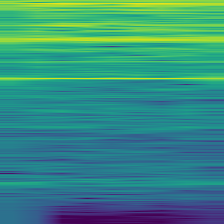
\includegraphics[width=\linewidth]{STFT_98_Normal_1_00000}
		\caption{Mel spectrogram}
	\end{subfigure}
	\hfill
	\begin{subfigure}{0.48\linewidth}
		\centering
		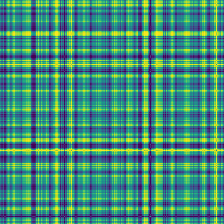
\includegraphics[width=\linewidth]{GADF_98_Normal_1_00000}
		\caption{GADF}
	\end{subfigure}
	
	\caption{Bearing vibration signal representations. (a) STFT spectrogram. (b) GADF image.}
	\label{representation}
	
\end{figure}

\subsubsection{Gramian Angular Field}

To address the limitations of the STFT spectrogram in encoding global temporal structures, the Gramian Angular Field (GAF) is introduced as a complementary representation. The GAF is a method that transforms one-dimensional time-series signals into two-dimensional images while preserving and encoding rich temporal correlation information \cite{11048665}. It was originally proposed to facilitate time-series classification through computer vision techniques \cite{10114345}, \cite{10281942}. The construction of a GAF representation involves three steps:

\begin{enumerate}
\item The time series $\boldsymbol{X} = \{x_1, x_2, \ldots, x_n\}$ is first normalized to the interval $[-1, 1]$ using min--max normalization, producing a normalized sequence $\boldsymbol{\tilde X} = \{\tilde{x_1}, \tilde{x_2}, \ldots, \tilde{x_n}\}$, where each $\tilde{x}_i$ is computed as

\begin{equation}
\tilde{x}_i = \frac{(x_i - \min \boldsymbol{X}) + (x_i - \max \boldsymbol{X})}{\max \boldsymbol{X} - \min \boldsymbol{X}}.
\label{normalization}
\end{equation}

\item The normalized values $\tilde{x}_i$ are then encoded as angular coordinates in a polar coordinate system. Specifically, each $\tilde{x}_i$ is mapped to a polar angle $\phi_i$, while the corresponding radial coordinate $r_i$ represents the temporal order of the sequence. This transformation is defined as

\begin{equation}
\begin{cases} 
\phi_i = \arccos(\tilde{x}_i), & -1 \leq \tilde{x}_i \leq 1,  \tilde{x}_i \in \boldsymbol{\tilde X} \\[4pt]
r_i = \dfrac{i}{n}, & i = 1, \ldots, n 
\end{cases},
\label{cosine angle}
\end{equation}

where $\phi_i$ denotes the polar angle of the $i$-th point and $r_i$ represents its normalized temporal position. This polar encoding ensures that the temporal ordering of the signal is preserved through the radial coordinate, while signal amplitude variations are encoded as angular deviations.

\item Finally, the GAF is constructed by aggregating the phase angles through either summation or difference operations, yielding two complementary variants: the Gramian Angular Summation Field (GASF), denoted as $\boldsymbol{G_s}$, and the Gramian Angular Difference Field (GADF), denoted as $\boldsymbol{G_d}$. Their formulations are defined as

\begin{equation}
\boldsymbol{G_s}(i,j) = \cos(\phi_i + \phi_j), \quad i,j = 1,\ldots,n
\label{eq:gasf}
\end{equation}

\begin{equation}
\boldsymbol{G_d}(i,j) = \sin(\phi_i - \phi_j), \quad i,j = 1,\ldots,n.
\label{eq:gadf}
\end{equation}
\end{enumerate}

The GAF representation offers several advantages that complement the Mel spectrogram. First, by encoding pairwise angular relationships between all time points, the GAF captures global temporal correlation structures that extend beyond the local receptive field of STFT-based representations. This property makes it particularly effective for detecting fault-induced irregularities in temporal dynamics, such as those caused by harmonic distortions or partial discharge events. Second, the min--max normalization in~\eqref{normalization} inherently suppresses the influence of absolute signal amplitude, making the GAF representation more robust to variations in signal gain and background noise levels compared with raw spectrogram representations. Furthermore, the polar encoding in~\eqref{cosine angle} provides a bijective mapping between the original time series and its angular representation, ensuring that temporal information is preserved without information loss.

In this study, the GADF variant is specifically adopted to complement the Mel spectrogram. Compared with GASF, which encodes angular summation, GADF focuses on angular differences and thereby exhibits higher sensitivity to abrupt temporal variations and asymmetric dynamic patterns \cite{11278186}. This property is particularly beneficial for bearing fault diagnosis, where abnormal operating conditions often produce irregular temporal fluctuations in the vibration signals. As shown in Fig.~\ref{representation}(b), the GADF encodes structured temporal dependencies from acoustic signals under normal operating conditions. The resulting image exhibits regular and symmetric patterns, reflecting stable temporal correlations and consistent signal dynamics. Such characteristics provide discriminative cues for distinguishing normal conditions from fault-induced irregular patterns.

For the experiments in this study, the GADF is computed with a sequence length of $n = 224$, matching the target image dimension. The angular difference variant (GADF) is selected rather than the summation variant (GASF) due to its superior sensitivity to abrupt temporal variations. The resulting GADF matrix is normalized to $[0, 1]$, converted to an 8-bit grayscale image, and subsequently mapped to a pseudo-color representation of size $224 \times 224$ using the Viridis colormap. Together, the Mel spectrogram and GADF constitute a complementary representation pair that jointly captures local spectral energy patterns and global temporal correlation structures, providing a comprehensive basis for the subsequent adaptive fusion stage.

\subsection{AW-DPCNN for Multi-Representation Fusion}
\label{sec:awdpcnn}

As discussed in Section~\ref{section2}, the STFT spectrogram and GADF provide fundamentally different yet complementary representations of bearing vibration signals. Specifically, the STFT spectrogram primarily characterizes local time--frequency energy distributions with uniform spectral resolution, whereas the GADF emphasizes global temporal dependencies and dynamic correlation structures. Owing to their distinct statistical properties and structural characteristics, directly combining these heterogeneous representations using conventional pixel-wise averaging or simple feature concatenation may fail to effectively capture their cross-modal relationships and may even introduce destructive interference, as demonstrated in the ablation study (Section~\ref{section4}). To address this issue, the proposed AW-DPCNN introduces a PCNN-inspired fusion mechanism with three key innovations: (i) dual-channel external stimuli that independently process Mel and GADF representations through representation-specific convolutional kernels; (ii) a contrast-guided adaptive weighting scheme that dynamically adjusts the relative contribution of each representation based on local saliency; and (iii) iterative pulse-coupled dynamics that propagate and reinforce structurally consistent features across multiple iterations while suppressing spurious activations.

The pulse coupling characteristic of PCNN enables dynamic interaction among neighboring feature responses, allowing salient structures shared across STFT and GADF representations to be synchronously enhanced while suppressing irrelevant or inconsistent activations~\cite{Li_2018}. Such a mechanism is particularly suitable for multi-representation fusion, where local spectral textures and global temporal correlation patterns coexist across different feature domains~\cite{kangEnhancementAlgorithmColor2021}. Moreover, the adaptive weighting strategy further regulates the contribution of each representation according to their fault-sensitive responses, thereby improving feature complementarity and discriminative capability.

Building upon these characteristics, the proposed AW-DPCNN integrates dual-channel processing, adaptive weighting, and multi-scale convolution to effectively model cross-representation dependencies and hierarchical feature interactions between STFT and GADF representations, ultimately enhancing bearing fault diagnosis performance. The key hyperparameters of the AW-DPCNN are summarized in Table~\ref{tab:awdpcnn_params}, and the detailed formulation of each component is presented below.

\subsubsection{Input Normalization}
To eliminate scale differences between two representations, each input is first normalized to the interval $[0,1]$ as
\begin{equation}
	\boldsymbol{\tilde{S}}_k(i,j) = \frac{\boldsymbol{S}_k(i,j) - \min\limits_{i,j} (\boldsymbol{S}_k(i,j))}{\max\limits_{i,j} (\boldsymbol{S}_k(i,j)) - \min\limits_{i,j} (\boldsymbol{S}_k(i,j)) + \epsilon}, k\in\{1,2\}
	\label{eq:normalization}
\end{equation}
where $\boldsymbol{S}_k(i,j)$ denotes the value of the $k$-th input representation at spatial location $(i,j)$, corresponding to the STFT spectrogram ($k=1$) or the GADF image ($k=2$). The variables $i$ and $j$ denote the pixel indices, and $\epsilon$ is a small positive constant preventing division by zero.

\subsubsection{Contrast-Guided Adaptive Weighting}
For each representation, the local mean of the normalized representation is computed as
\begin{equation}
	\boldsymbol{\mu}_k(i,j) = \frac{1}{|\boldsymbol{\Omega}|}
	\sum_{(p,q)\in \boldsymbol{\Omega}} \boldsymbol{\tilde{S}}_k(p,q),
	\label{eq:local_mean}
\end{equation}
where $\boldsymbol{\Omega}$ denotes the local neighborhood centered at each pixel location, and $|\boldsymbol{\Omega}|$ represents the number of elements in the neighborhood.

The corresponding local contrast is defined as
\begin{equation}
	C_k(i,j) = \sqrt{ \left| \mathbb{E}_\Omega \left[ \tilde{S}_k^2 \right] - \mu_k^2(i,j) \right| },
	\label{eq:eq:local_contrast}
\end{equation}
where $\mathbb{E}[\cdot]$ denotes local averaging within $\boldsymbol{\Omega}$.

Local contrast operators $C_1(i,j)$ and $C_2(i,j)$ are computed to quantify the saliency of STFT and GADF representations at each spatial location. To emphasize the dominant representation, a contrast amplification factor $\gamma$ is introduced to construct adaptive fusion weights as follows
\begin{equation}
	\beta_1(i,j) = 
	\frac{\gamma C_1(i,j)}
	{\gamma C_1(i,j) + C_2(i,j) + \epsilon},
	\label{eq:beta1}
\end{equation}
\begin{equation}
	\beta_2(i,j) = 
	\frac{C_2(i,j)}
	{\gamma C_1(i,j) + C_2(i,j) + \epsilon},
	\label{eq:beta2}
\end{equation}
the above formulation ensures $\beta_1(i,j) + \beta_2(i,j) \approx 1$, enabling contrast-driven dynamic weighting.

\subsubsection{Dual-Channel PCNN}
Let $\boldsymbol{L}^n(i,j)$, $\boldsymbol{T}^n(i,j)$, and $\boldsymbol{Y}^n(i,j)$ denote the linking term, dynamic threshold, and binary pulse output, respectively, where $n$ denotes the current iteration and $n \in [1, N]$, with $N$ being the total number of iterations. The neural states are initialized as
\begin{equation}
	\boldsymbol{L}^0(i,j) = \boldsymbol {0}, \quad 
	\boldsymbol{T}^0(i,j) = \boldsymbol {0}, \quad 
	\boldsymbol{Y}^0(i,j) = \boldsymbol {0}.
	\label{eq:initialization}
\end{equation}

At the $n$-th iteration, the external stimulus from two channels is defined as
\begin{equation}
	\boldsymbol{F}_1^n(i,j) = (\boldsymbol{W}_1 * \boldsymbol{Y}^{n-1})(i,j) + \boldsymbol{\tilde{S}}_1(i,j)
	\label{eq:f1_update}
\end{equation}
\begin{equation}
	\boldsymbol{F}_2^n(i,j) = (\boldsymbol{W}_2 * \boldsymbol{Y}^{n-1})(i,j) + \boldsymbol{\tilde{S}}_2(i,j),
	\label{eq:f2_update}
\end{equation}
where $\boldsymbol{W}_1$ and $\boldsymbol{W}_2$ denote the convolutional kernels corresponding to the STFT and GADF channels, respectively, and $*$ represents the convolution operation. Considering the distinct structural characteristics of the two representations, representation-specific convolutional kernels are introduced in the dual-channel architecture. Specifically, stripe-shaped kernels are applied to the STFT channel to emphasize frequency continuity and harmonic structures, while symmetric kernels are used for the GADF channel to capture temporal periodicity and global correlation patterns. In this study, $\boldsymbol{W}_1$, $\boldsymbol{W}_2$, and $\boldsymbol{M}$ are structural design choices grounded in the physical interpretation of each representation, not free hyperparameters.

The internal linking state is updated by
\begin{equation}
	\boldsymbol{L}^n(i,j) = e^{-\alpha_L} \boldsymbol{L}^{n-1}(i,j) + (\boldsymbol{M} * \boldsymbol{Y}^{n-1})(i,j),
	\label{eq:linking_update}
\end{equation}
where $\alpha_L$ is the decay coefficient and $\boldsymbol M$ represents the coupling matrix.

The total neuron input is then given by
\begin{equation}
	\boldsymbol{U}^n(i,j) = \boldsymbol{L}^n(i,j)\Big(1 + \beta_1 \boldsymbol{F}_1^n(i,j)\Big)
	\Big(1 + \beta_2 \boldsymbol{F}_2^n(i,j)\Big) + \sigma,
	\label{eq:internal_activity}
\end{equation}
where $\sigma$ is a stabilization constant.

The pulse output is determined by a threshold comparison as follows
\begin{equation}
	\boldsymbol{Y}^n(i,j) =
	\begin{cases}
		1, & \boldsymbol{U}^n(i,j) > \boldsymbol{T}^{n-1}(i,j) \\
		0, & \text{otherwise}
	\end{cases}.
	\label{eq:pulse_output}
\end{equation}

The dynamic threshold evolves according to
\begin{equation}
	\boldsymbol{T}^n(i,j) = e^{-\alpha_T} \boldsymbol{T}^{n-1}(i,j) + V_T \boldsymbol{Y}^n(i,j),
	\label{eq:threshold_update}
\end{equation}
where $\alpha_T$ controls threshold decay and $V_T$ is the amplification coefficient.

\subsubsection{Fused Representation}
The accumulated neural response after $N$ iterations is
\begin{equation}
	\boldsymbol{U}_{\mathrm{sum}}(i,j)=\sum_{n=1}^{N} \boldsymbol{U}^{n}(i,j),
\end{equation}
and the final fused representation is obtained via normalization as
\begin{equation}
	\boldsymbol{F}(i,j)=
	\frac{\boldsymbol{U}_{\mathrm{sum}}(i,j)-\min\limits_{i,j} \boldsymbol{U}_{\mathrm{sum}}(i,j)}
	{\max\limits_{i,j} \boldsymbol{U}_{\mathrm{sum}}(i,j)-\min\limits_{i,j} \boldsymbol{U}_{\mathrm{sum}}(i,j)+\epsilon}.
\end{equation}

Through the proposed adaptive fusion mechanism, STFT and GADF representations are no longer combined with fixed weights. Instead, the neuron state is dynamically modulated in a demand-driven manner, i.e., regions dominated by spectral variations are mainly governed by the STFT spectrogram, while regions with stronger temporal correlations rely more on GADF. This adaptive strategy effectively suppresses fusion artifacts while enhancing the discriminative capability of fused representations.

The overall architecture of the proposed AW-DPCNN is illustrated in Fig.~\ref{AW-DPCNN}. By integrating STFT spectral perception and GADF temporal encoding within a unified adaptive fusion framework, the proposed AW-DPCNN produces robust and discriminative representations for bearing fault diagnosis. The qualitative effectiveness of the proposed adaptive fusion mechanism is further analyzed through feature visualization in Section~\ref{section4}.
\begin{figure}[!htbp]
	\centering
	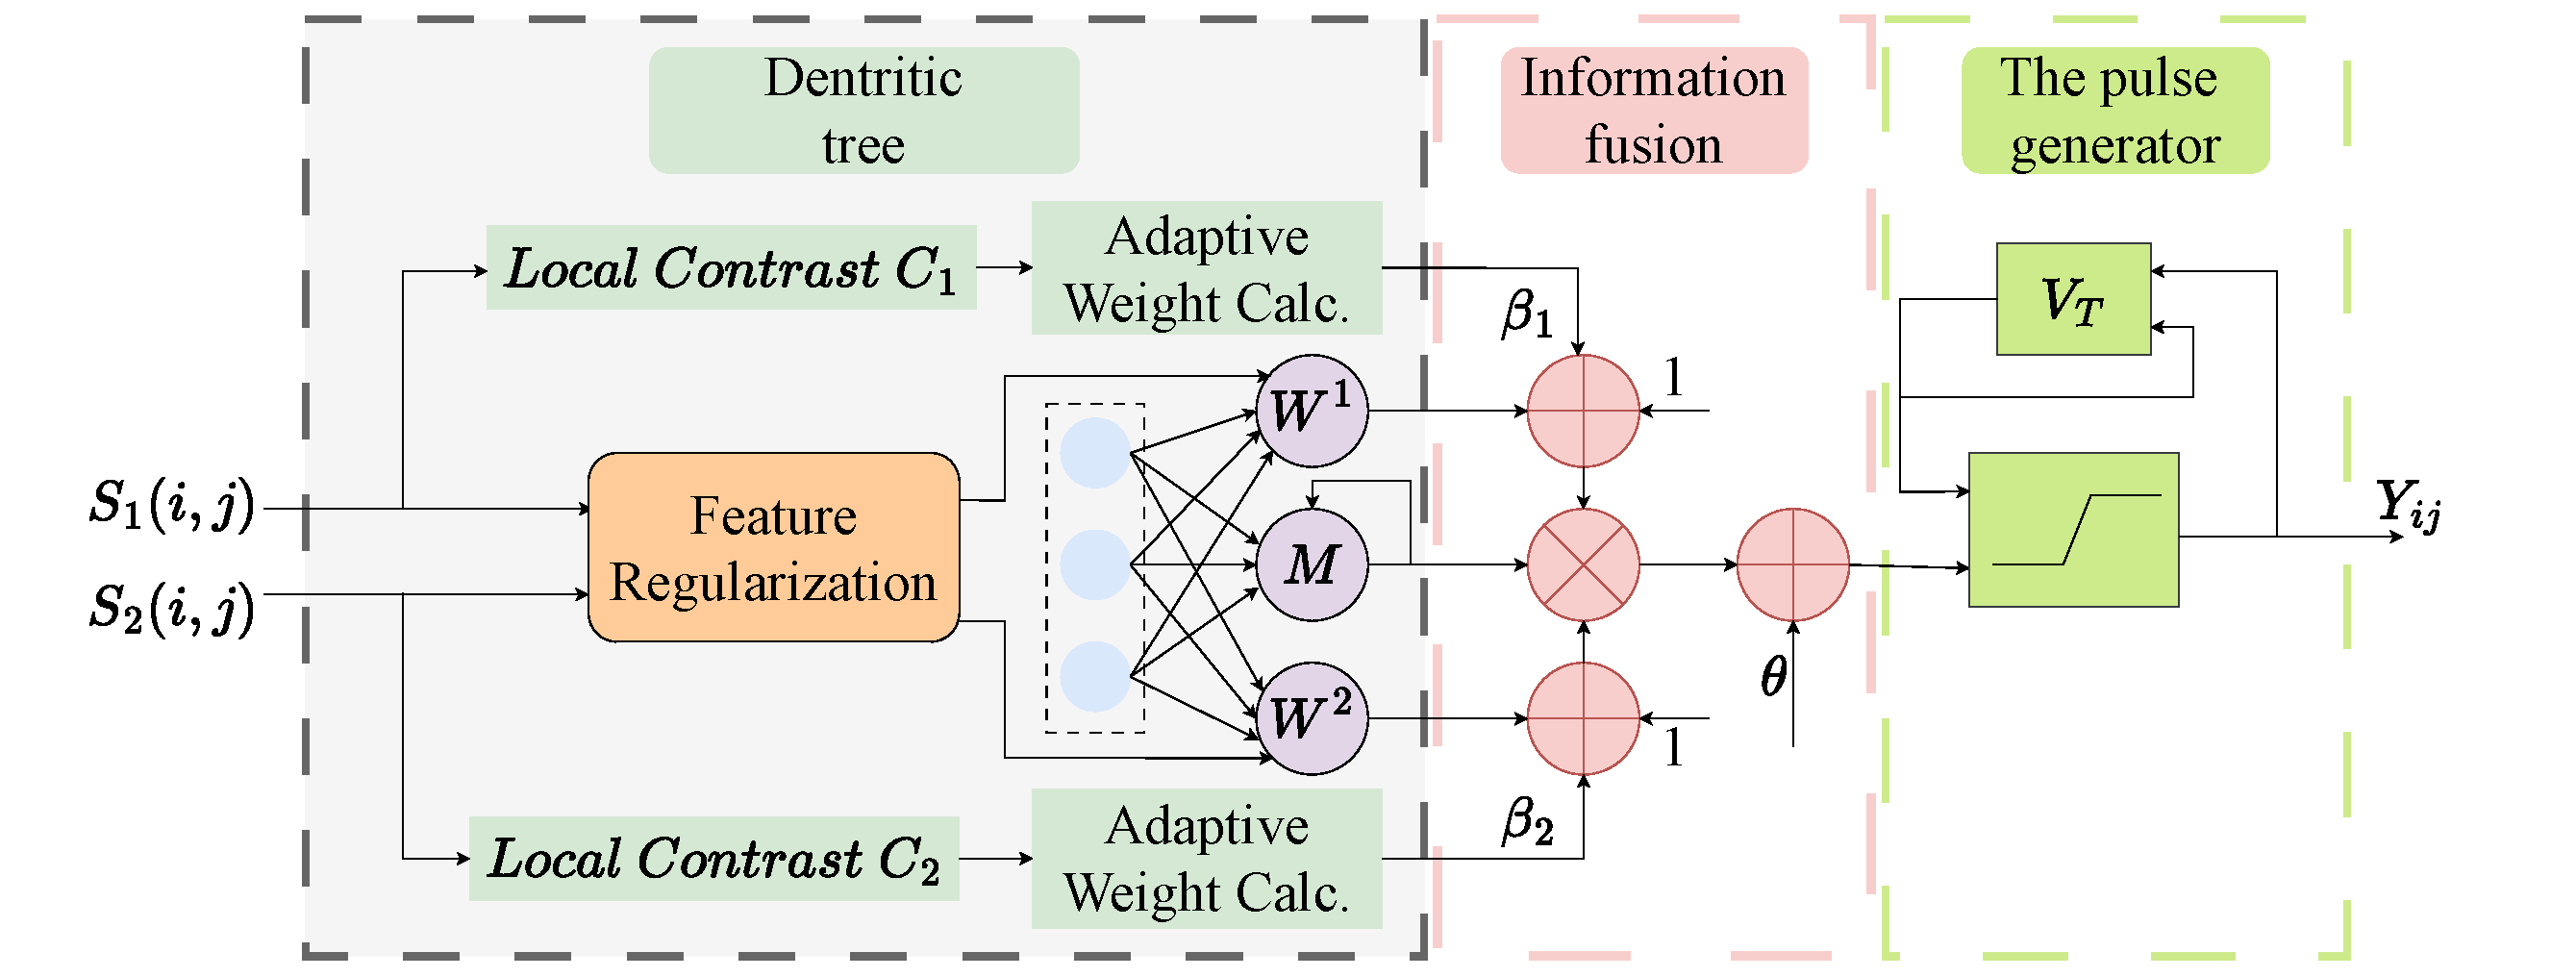
\includegraphics[width=\linewidth]{AW-DPCNN/AW-DPCNN}
	\caption{Architecture of the proposed adaptive weighted dual-channel PCNN (AW-DPCNN) for multi-representation signal fusion.}
	\label{AW-DPCNN}                       
\end{figure}


\begin{figure*}[!htbp] 
\centering
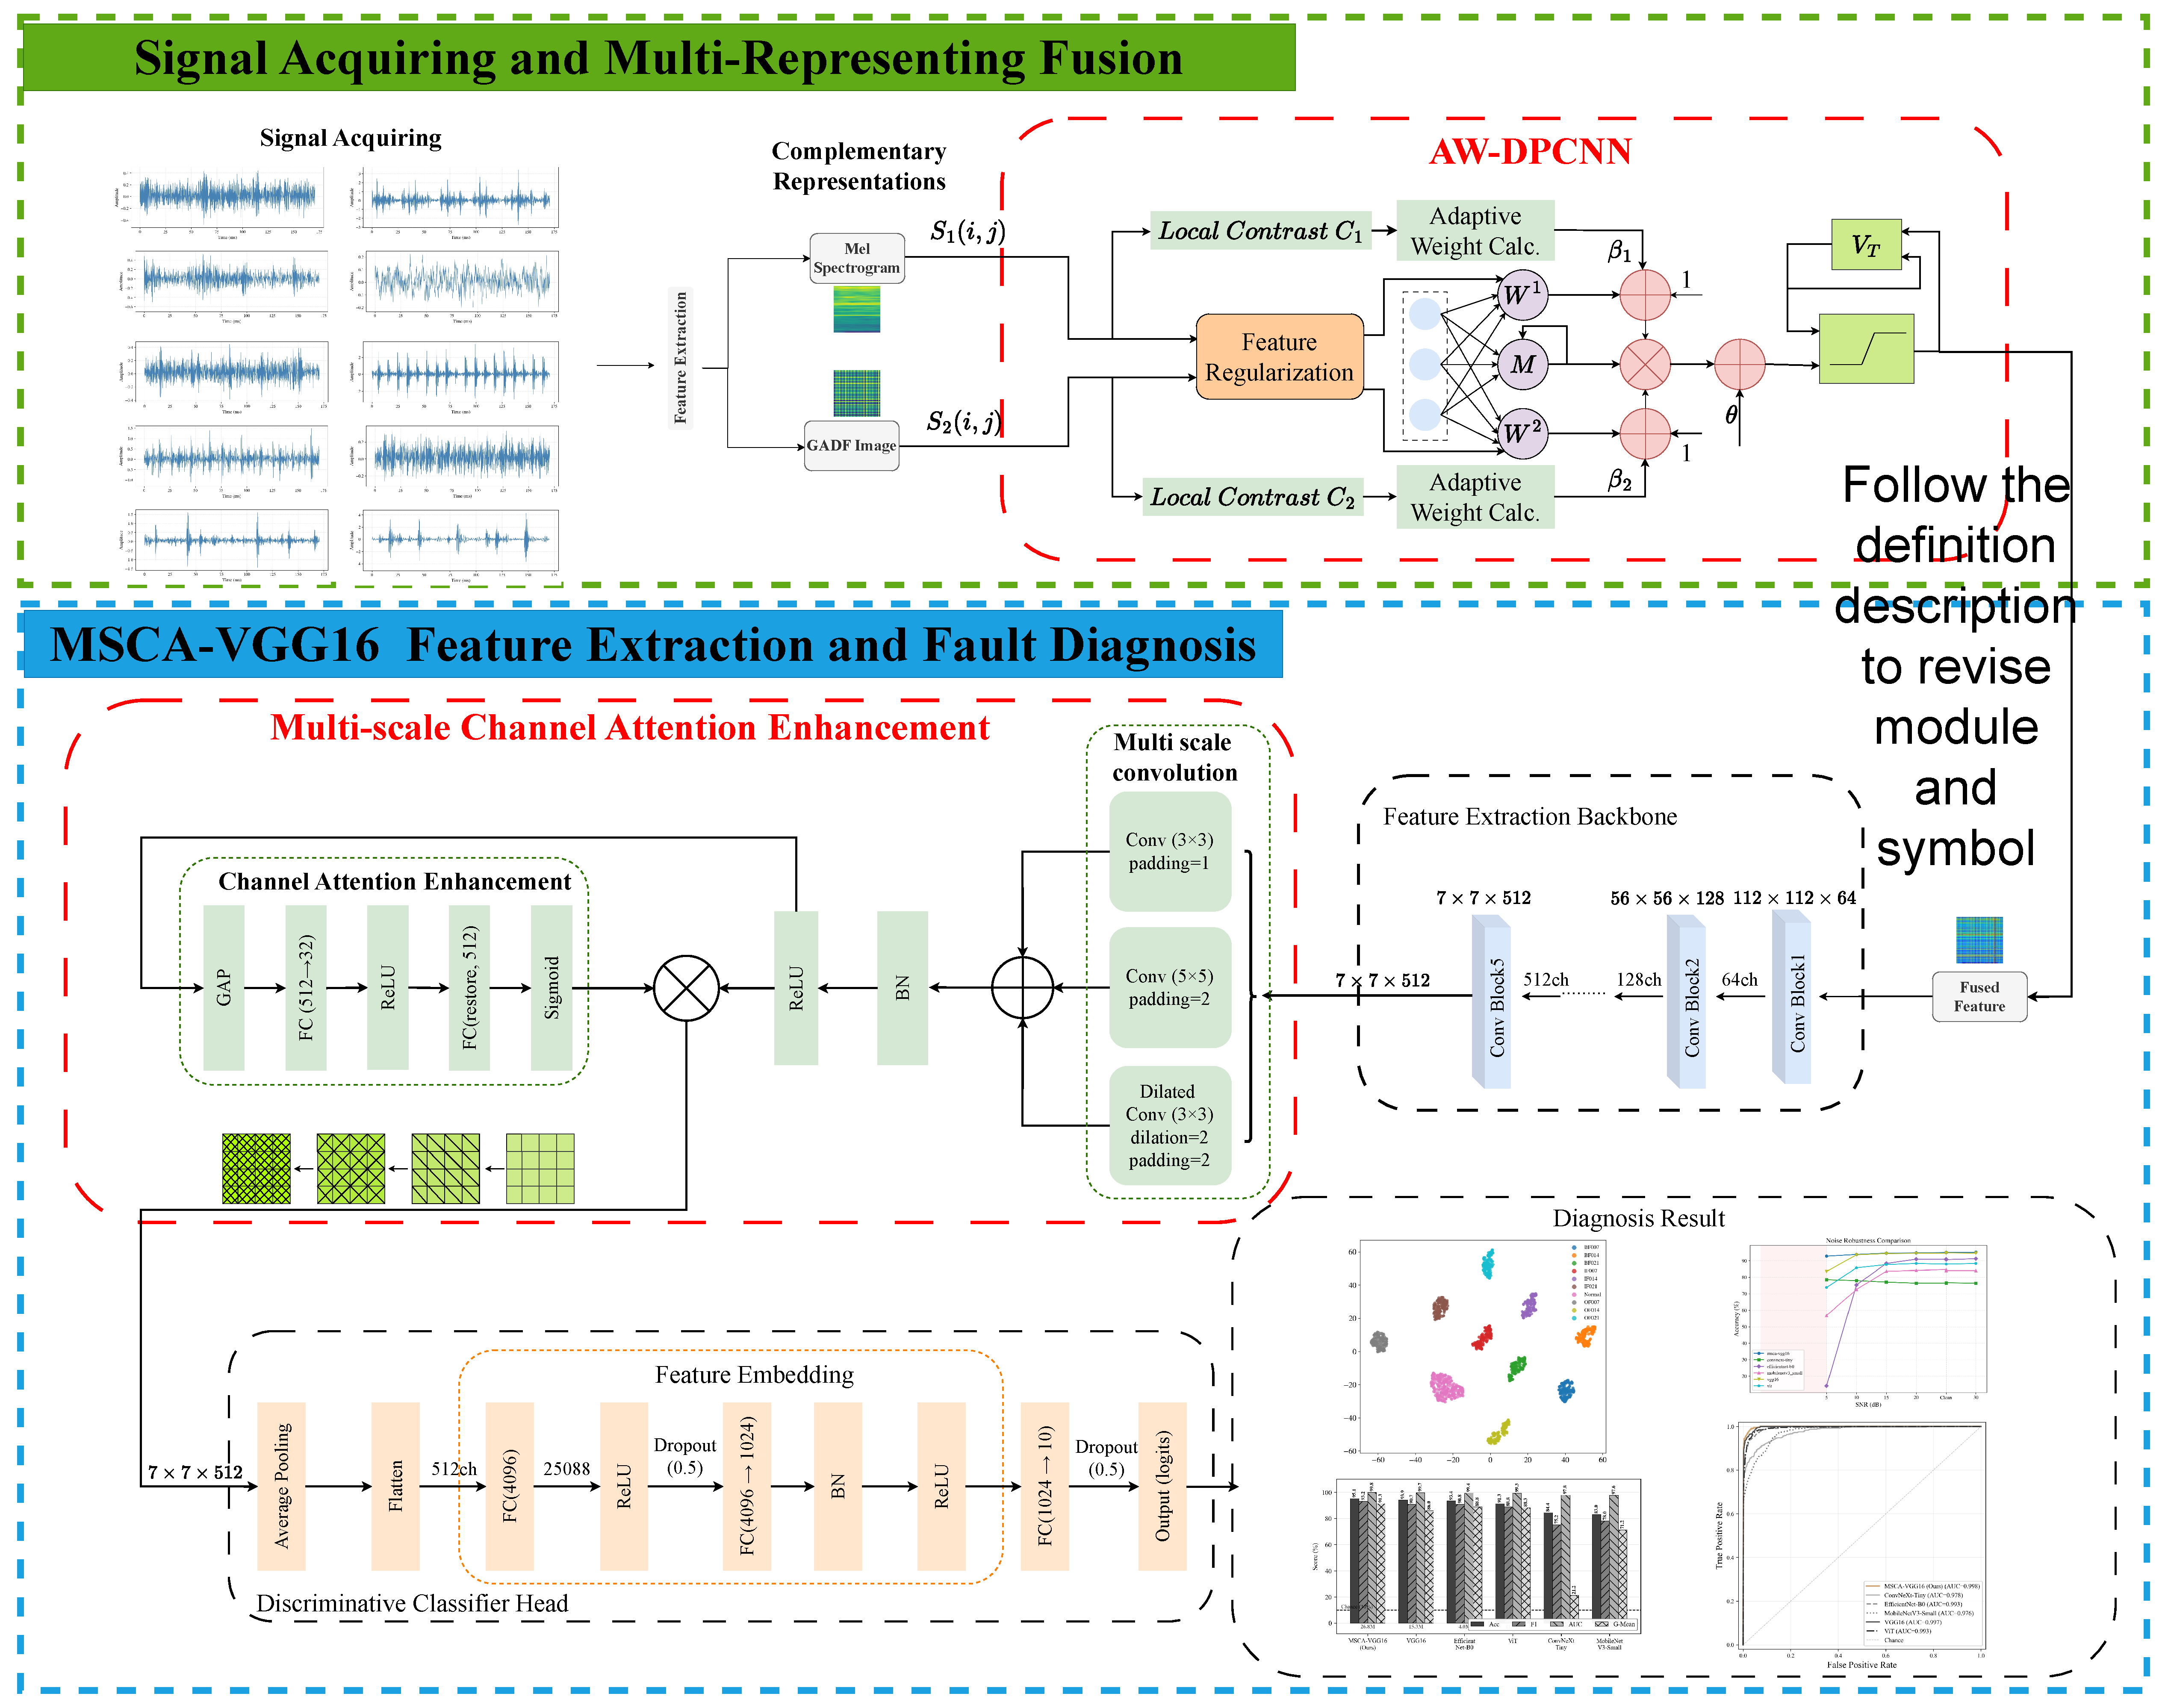
\includegraphics[width=\linewidth]{overview/overview.pdf}
\caption{}
\label{}
\end{figure*}

\subsection{MSCA-VGG16 for Fused Representation Classification}
\label{sec:msca_vgg16}

\subsubsection{Design Philosophy and Overview}

The fused representations $\boldsymbol{S}_{\mathrm{fused}}$ generated by AW-DPCNN simultaneously encode local time--frequency energy variations from STFT spectrograms and global temporal correlation structures from GADF encoding. These heterogeneous features exhibit distinct statistical distributions: Mel-derived components emphasize localized spectral textures, while GADF-derived components reveal long-range structural dependencies. Conventional convolutional networks with fixed receptive fields and uniform channel treatment are ill-suited to jointly exploit such complementary information. To address this, we develop a Multi-Scale Channel Attention enhanced network (MSCA-VGG16) built upon three design principles: (i) \emph{multi-scale receptive field alignment} to capture fault patterns spanning different temporal and spectral granularities; (ii) \emph{dynamic channel recalibration} via squeeze-and-excitation to suppress noise-dominated frequency bands while amplifying fault-sensitive responses; and (iii) \emph{compact discriminative embedding} to project high-dimensional convolutional features into a lower-dimensional space that enhances intra-class compactness and inter-class separability.

The overall architecture is a modular composition of a convolutional backbone $\mathcal{B}(\cdot)$, a multi-scale channel attention module $\mathcal{M}(\cdot)$, global pooling $\mathcal{P}(\cdot)$, an embedding projection $\mathcal{E}(\cdot)$, and a linear classifier $\mathcal{F}_{cls}(\cdot)$. The forward mapping from input $\boldsymbol{X}$ to predicted class probabilities $\hat{\mathbf{y}}$ is

\begin{equation}
\hat{\mathbf{y}} = \mathcal{F}_{cls}\big(\mathcal{E}\big(\mathcal{P}\big(\mathcal{M}\big(\mathcal{B}(\boldsymbol{X})\big)\big)\big)\big),
\label{eq:cls_pipeline}
\end{equation}

where $\boldsymbol{X} \in \mathbb{R}^{H_0 \times W_0 \times 3}$ denotes the AW-DPCNN fused pseudo-color image of spatial size $H_0 \times W_0$. The following subsections detail each component.

\subsubsection{Convolutional Backbone}

The backbone $\mathcal{B}(\cdot)$ serves as a hierarchical feature extractor that maps the fused input image to a rich spatial feature representation. It consists of a stack of convolutional stages with progressively increasing channel dimensionality and decreasing spatial resolution, implemented through strided convolutions or pooling operations. Formally, the backbone can be any deep convolutional architecture that accepts an RGB image and produces a feature map

\begin{equation}
\boldsymbol{F} = \mathcal{B}(\boldsymbol{X}), \quad \boldsymbol{F} \in \mathbb{R}^{H \times W \times C},
\label{eq:feature_map}
\end{equation}

where $H$, $W$, and $C$ denote the spatial height, width, and number of channels of the output feature map, respectively. The spatial dimensions $H$ and $W$ are determined by the cumulative downsampling factor of the backbone, while $C$ corresponds to the channel capacity of the final convolutional stage.

In this study, VGG16 with batch normalization (VGG16-BN)~\cite{zhangFaultDiagnosisRecognition2024} is selected as the primary convolutional backbone for the MSCA framework. The selection is guided by three interrelated considerations: architectural compatibility with the auxiliary modules, experimental interpretability, and the avoidance of confounding mechanisms.

\textbf{Architectural compatibility.} The MSCA framework attaches three auxiliary modules—the multi-scale convolution (MS) module, the squeeze-and-excitation channel attention (CA) module, and the compact embedding head (EH)—onto the backbone's output feature map. This imposes two structural requirements on the backbone: (i) a linear, single-path feedforward topology that permits clean insertion of auxiliary modules without routing around residual branches, and (ii) a sufficiently rich output channel capacity to support the MS module's parallel branches without channel competition. VGG16-BN satisfies both requirements: its architecture is a pure sequential stack of $3\times3$ convolutional blocks with no skip connections, identity shortcuts, or built-in attention mechanisms, providing a uniform insertion surface for the MS, CA, and EH modules. Its final convolutional stage outputs 512-channel feature maps at $7\times7$ spatial resolution, offering ample representational headroom for the three parallel multi-scale branches to extract complementary patterns. In contrast, architectures with residual connections introduce branching topologies that complicate the definition of insertion points: the MS module's parallel branches would require separate identity paths, conflating the contribution of multi-scale processing with that of the backbone's own skip structure. Architectures with built-in SE modules (e.g., EfficientNet's MBConv blocks) create redundancy with the CA module, making it impossible to attribute performance gains unambiguously. Vision Transformers lack the convolutional inductive bias and spatial hierarchy that the MS module relies upon to capture patterns at different spatial granularities.

\textbf{Experimental interpretability.} A central objective of this study is to evaluate the effectiveness of the MS, CA, and EH modules in enhancing feature discrimination for fused representations. Isolating the contribution of these modules from the backbone's inherent properties requires a backbone that provides a neutral starting point—that is, an architecture with no attention, no multi-scale processing, and no skip connections. VGG16-BN, being the most canonical deep convolutional architecture, provides precisely such a baseline. Every performance gain can therefore be unambiguously attributed to the proposed modules rather than to synergies with the backbone's own design. Furthermore, VGG16 has a single well-defined variant with batch normalization, eliminating the degrees of freedom associated with selecting among multiple variants (e.g., ResNet-18/34/50/101) and thereby enhancing reproducibility.

\textbf{Avoidance of confounding mechanisms.} ResNet's skip connections inherently provide a form of implicit multi-scale gradient flow that could partially mask the benefit of the MS module. EfficientNet's MBConv blocks already contain SE operations, rendering the CA module redundant and preventing a clean ablation of channel attention. ViT's self-attention mechanism operates globally by design, which conflicts with the locally-grounded multi-scale receptive fields of the MS branches. VGG16-BN possesses none of these mechanisms, serving as a ``blank canvas'' on which the effect of each proposed module can be independently assessed.

To validate this selection empirically, a comparative experiment is conducted in Section~\ref{sec:backbone_comparison}, where the MSCA framework is instantiated with several alternative backbones, including EfficientNet-B0, MobileNetV3-Small, ConvNeXt-Tiny, and ViT. The results confirm that VGG16-BN, when augmented with the MS, CA, and EH modules, consistently achieves the most favorable accuracy--efficiency trade-off on the target diagnostic task, corroborating the architectural analysis presented above.

\subsubsection{Multi-Scale Convolution Module}

Fault signatures in fused representations manifest at multiple scales: fine-grained local anomalies (e.g., impulsive spectral lines), mid-range harmonic patterns, and long-range structural correlations across time and frequency. A single receptive field cannot simultaneously capture all three. To align the network's perceptual field with this multi-scale nature, we introduce a multi-scale convolution (MS) module $\psi_{\mathrm{MS}}(\cdot)$ comprising $S$ parallel branches with different effective receptive fields:

\begin{equation}
\boldsymbol{F}_{\mathrm{ms}} = \psi_{\mathrm{MS}}(\boldsymbol{F}) = \sum_{i=1}^{S} \psi_i(\boldsymbol{F}; \boldsymbol{\Theta}_i),
\label{eq:multi_scale_feature}
\end{equation}

where $\psi_i(\cdot; \boldsymbol{\Theta}_i)$ denotes the $i$-th convolutional branch parameterized by $\boldsymbol{\Theta}_i$. Each branch employs a distinct kernel configuration to capture patterns at a specific scale: a standard small-kernel convolution for local fine-grained textures, a larger-kernel convolution for mid-range structural features, and a dilated convolution that expands the receptive field without additional parameters for long-range dependencies. Each branch preserves the channel dimensionality $C$ of the backbone output.

The outputs are fused via element-wise summation, which encourages each branch to specialize in complementary scales. The aggregated feature map is normalized and activated:

\begin{equation}
\boldsymbol{F}_{\mathrm{act}} = \delta\big(\mathrm{BN}(\boldsymbol{F}_{\mathrm{ms}})\big),
\label{eq:active_feature}
\end{equation}

where $\delta(\cdot) = \max(0, \cdot)$ is the ReLU activation and $\mathrm{BN}(\cdot)$ denotes batch normalization. The specific kernel sizes, dilation rates, and the number of branches $S$ are provided as hyperparameter configurations in the experiment section (Section~\ref{section4}).

\subsubsection{Squeeze-and-Excitation Channel Attention}

Different frequency bands in the fused representation carry unequal diagnostic information. Some channels encode fault-critical spectral components, while others are dominated by background noise or redundant textures. To dynamically recalibrate channel-wise responses, we adopt a squeeze-and-excitation (SE) mechanism~\cite{hu2018squeeze} after the multi-scale fusion stage.

Let $\boldsymbol{F}_{\mathrm{act}} \in \mathbb{R}^{H \times W \times C}$ be the input to the SE module. The \emph{squeeze} operation aggregates spatial information into a channel descriptor $\boldsymbol{z} \in \mathbb{R}^{C}$ via global average pooling:

\begin{equation}
z_c = \frac{1}{H W} \sum_{i=1}^{H} \sum_{j=1}^{W} \boldsymbol{F}_{\mathrm{act}}(i, j, c), \quad c = 1, \dots, C.
\label{eq:se_squeeze}
\end{equation}

The \emph{excitation} operation models channel-wise dependencies through a bottleneck structure:

\begin{equation}
\boldsymbol{s} = \sigma\big(\boldsymbol{W}_2 \, \delta(\boldsymbol{W}_1 \boldsymbol{z})\big),
\label{eq:se_excitation}
\end{equation}

where $\boldsymbol{W}_1 \in \mathbb{R}^{\frac{C}{r} \times C}$ and $\boldsymbol{W}_2 \in \mathbb{R}^{C \times \frac{C}{r}}$ are learnable weight matrices, $r$ is the channel reduction ratio controlling the bottleneck capacity, and $\sigma(\cdot)$ is the sigmoid function. The output $\boldsymbol{s} = [s_1, \dots, s_C]^\top$ represents per-channel attention weights in $[0, 1]$. The refined feature map is obtained by channel-wise rescaling:

\begin{equation}
\boldsymbol{F}_{\mathrm{att}}(i, j, c) = s_c \cdot \boldsymbol{F}_{\mathrm{act}}(i, j, c).
\label{eq:attention_feature}
\end{equation}

This mechanism allows the network to emphasize channels containing fault-discriminative information (e.g., frequency bands with strong harmonic signatures) while attenuating noise-dominated channels. The reduction ratio $r$ is specified in the experiment configuration.

\subsubsection{Compact Discriminative Embedding Head}

Conventional CNN classifiers often employ large fully-connected layers that are prone to overfitting on small-scale fault diagnosis datasets and introduce substantial parameter redundancy~\cite{9770845}. We replace these with a compact embedding head that projects high-dimensional convolutional features into a low-dimensional discriminative space, promoting intra-class compactness and inter-class separation while reducing the parameter count.

First, the spatially refined feature map $\boldsymbol{F}_{\mathrm{att}}$ is collapsed via global average pooling and flattened:

\begin{equation}
\boldsymbol{f}_0 = \mathrm{Flatten}\big(\mathrm{AvgPool}(\boldsymbol{F}_{\mathrm{att}})\big) \in \mathbb{R}^{C}.
\label{eq:flatten_feature}
\end{equation}

A fully-connected projection layer extracts high-level features:

\begin{equation}
\boldsymbol{f}_1 = \delta\big(\boldsymbol{W}_{\!fc1}\, \boldsymbol{f}_0\big), \quad \boldsymbol{W}_{\!fc1} \in \mathbb{R}^{D_1 \times C},
\label{eq:fc1_feature}
\end{equation}

followed by dropout for regularization. A compact embedding layer then projects $\boldsymbol{f}_1$ into a $d$-dimensional discriminative space:

\begin{equation}
\boldsymbol{e} = \delta\big(\mathrm{BN}(\boldsymbol{W}_{\!e}\, \boldsymbol{f}_1)\big), \quad \boldsymbol{e} \in \mathbb{R}^{d},
\label{eq:embedding}
\end{equation}

where $\boldsymbol{W}_{\!e} \in \mathbb{R}^{d \times D_1}$. Batch normalization is applied prior to ReLU to stabilize the feature distribution, and dropout follows the embedding layer. Finally, the class logits are obtained via a linear classifier:

\begin{equation}
\hat{\boldsymbol{y}} = \mathrm{softmax}(\boldsymbol{W}_{\!c}\, \boldsymbol{e}), \quad \boldsymbol{W}_{\!c} \in \mathbb{R}^{K \times d},
\label{eq:classifier}
\end{equation}

where $K$ is the number of fault categories. The dimensions $D_1$ (projection layer width) and $d$ (embedding dimensionality), as well as the dropout probability, are treated as hyperparameters whose concrete values are given in Section~\ref{section4}. The entire network is optimized by minimizing the cross-entropy loss:

\begin{equation}
\mathcal{L}_{\mathrm{CE}} = -\sum_{k=1}^{K} y_k \log \hat{y}_k,
\label{eq:cross_entropy_loss}
\end{equation}

where $\boldsymbol{y} = [y_1, \dots, y_K]^\top$ is the one-hot ground-truth label. In practice, a class-weighted variant $\mathcal{L}_{\mathrm{wCE}}$ is employed to counteract dataset imbalance (Section~\ref{section4}).

\subsubsection{Forward Pass Algorithm}

Algorithm~\ref{alg:msca_vgg16} summarizes the complete forward pass of the proposed MSCA-VGG16 network from the fused input image to the predicted class probabilities.

\begin{algorithm}
\caption{Forward Pass of MSCA-VGG16}
\label{alg:msca_vgg16}
\begin{algorithmic}[1]
\Require Fused AW-DPCNN image $\boldsymbol{X} \in \mathbb{R}^{H_0 \times W_0 \times 3}$
\State Extract backbone feature map $\boldsymbol{F}$ using Eq.~\ref{eq:feature_map}.
\State Compute multi-scale feature $\boldsymbol{F}_{\mathrm{ms}}$ using Eq.~\ref{eq:multi_scale_feature}.
\State Apply BatchNorm and ReLU to obtain $\boldsymbol{F}_{\mathrm{act}}$ using Eq.~\ref{eq:active_feature}.
\State Squeeze spatial information into channel descriptor $\boldsymbol{z}$ using Eq.~\ref{eq:se_squeeze}.
\State Compute channel attention weights $\boldsymbol{s}$ using Eq.~\ref{eq:se_excitation}.
\State Obtain channel-refined feature $\boldsymbol{F}_{\mathrm{att}}$ using Eq.~\ref{eq:attention_feature}.
\State Apply global average pooling and flatten to obtain $\boldsymbol{f}_0$ using Eq.~\ref{eq:flatten_feature}.
\State Project to high-level features $\boldsymbol{f}_1$ using Eq.~\ref{eq:fc1_feature}, then apply dropout.
\State Compute compact embedding $\boldsymbol{e}$ using Eq.~\ref{eq:embedding}, then apply dropout.
\State Produce class probabilities $\hat{\boldsymbol{y}}$ using Eq.~\ref{eq:classifier}.
\Ensure Predicted probabilities $\hat{\boldsymbol{y}} \in \mathbb{R}^{K}$, optimized via Eq.~\ref{eq:cross_entropy_loss}.
\end{algorithmic}
\end{algorithm}

\subsection{Training Strategy}

The MSCA-VGG16 classification network is trained using a supervised learning protocol with the following configuration. All experiments adopt the AdamW optimizer~\cite{loshchilov2017adamw} with an initial learning rate of $\eta = 1 \times 10^{-4}$ and a weight decay of $\lambda = 1 \times 10^{-3}$, which provides adaptive learning rate scaling with decoupled weight regularization for improved generalization. A ReduceLROnPlateau learning rate scheduler is employed, which reduces the learning rate by a factor of $0.5$ when the validation F1-score does not improve for $5$ consecutive epochs, with a minimum learning rate of $1 \times 10^{-6}$. The batch size is set to $32$ and the maximum number of training epochs is set to $30$.

To mitigate the adverse effects of class imbalance inherent in practical bearing vibration datasets, a class-weighted cross-entropy loss is adopted. Specifically, the weight $w_k$ for class $k$ is computed as
\begin{equation}
w_k = \frac{N_{\mathrm{total}}}{K \cdot N_k},
\label{eq:class_weight}
\end{equation}
where $N_{\mathrm{total}}$ denotes the total number of training samples, $K$ is the number of fault categories, and $N_k$ is the number of training samples belonging to class $k$. The weighted cross-entropy loss is then formulated as
\begin{equation}
\mathcal{L}_{\mathrm{wCE}} = -\frac{1}{B} \sum_{i=1}^{B} w_{y_i} \sum_{k=1}^{K} \boldsymbol{y}_{i,k} \log \hat{\boldsymbol{y}}_{i,k},
\label{eq:weighted_ce}
\end{equation}
where $B$ is the batch size, $y_i$ is the ground-truth label of the $i$-th sample, $\boldsymbol{y}_{i,k}$ is the $k$-th entry of the one-hot encoded label vector, and $\hat{\boldsymbol{y}}_{i,k}$ is the predicted probability for class $k$. This weighting strategy ensures that minority classes receive proportionally larger loss contributions, preventing the model from being biased toward majority classes.

To improve generalization and prevent overfitting, standard data augmentation techniques are applied during training, including random horizontal flipping with a probability of $0.5$ and random rotation within $\pm 10^{\circ}$. Input images are normalized using the ImageNet statistics (mean $= [0.485, 0.456, 0.406]$, standard deviation $= [0.229, 0.224, 0.225]$), which aligns with the pretrained VGG16-BN backbone and stabilizes the early stages of training.

Early stopping is employed to prevent overfitting, where training is terminated if the validation macro-averaged F1-score does not improve for $15$ consecutive epochs. The model checkpoint with the highest validation F1-score is retained for final evaluation on the held-out test set. To ensure reproducibility and statistical reliability, all key experiments are repeated over three independent trials with different random seeds ($42$, $123$, $456$), and the results are reported as mean $\pm$ standard deviation across the three trials. The training pipeline is implemented using PyTorch 2.11 with \texttt{torch.compile} acceleration enabled for improved computational efficiency on CUDA-compatible GPUs.





\section{Dataset and Experiments}
\label{section4}
\subsection{Dataset Construction and Preprocessing}
\label{Dataset Construction and Preprocessing}

The Case Western Reserve University (CWRU) bearing dataset~\cite{alonso-gonzalezBearingFaultDiagnosis2023} is employed as the primary benchmark for evaluating the proposed method. The experimental test stand, shown in Fig.~\ref{fig:cwru_teststand}, consists of a 2-hp motor, a torque transducer/encoder, a dynamometer, and control electronics. Vibration data were collected using accelerometers mounted at both the drive-end (DE) and fan-end (FE) of the motor housing, at sampling rates of 12~kHz and 48~kHz.

\begin{figure}[!htbp]
	\centering
	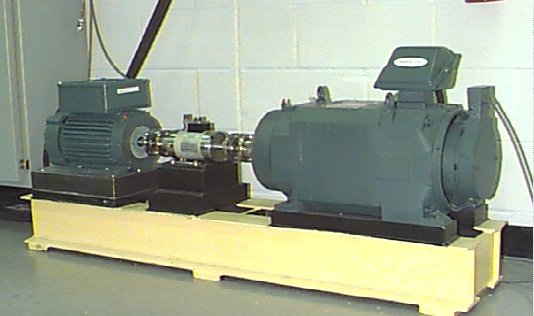
\includegraphics[width=\linewidth]{equipment/CWRU_teststand}
	\caption{CWRU bearing test stand. Vibration signals were collected from accelerometers at the drive-end and fan-end positions under four operating loads (0--3 hp).}
	\label{fig:cwru_teststand}
\end{figure}

Single-point faults of diameters 0.007, 0.014, and 0.021 inches were separately introduced to the ball, inner race, and outer race (at the 6 o'clock load zone position) using electro-discharge machining. Together with the healthy baseline condition, this yields ten fault categories as listed in Table~\ref{tab:operating_conditions}. Each fault class contains four source recordings of approximately 10~seconds duration; the normal baseline recordings are approximately 40~seconds long.

For dataset construction, the raw vibration signals are segmented into overlapping windows and converted into pseudo-color fused images through the AW-DPCNN pipeline. Three dataset variants are constructed to support comprehensive evaluation:

\begin{enumerate}
\item \textbf{CWRU 12k DE (primary benchmark):} 12~kHz drive-end signals with window length 2048 samples (170.7~ms) and hop length 1024 samples (85.3~ms). FFT window size $N_{\text{FFT}}=1024$, yielding 11.7~Hz/bin frequency resolution. Maximum frequency $f_{\max}=6$~kHz (full Nyquist bandwidth at 12~kHz sampling).
\item \textbf{CWRU 12k FE (cross-sensor generalization):} 12~kHz fan-end signals with identical time--frequency parameters to the 12k DE dataset, enabling evaluation of sensor-position transferability.
\item \textbf{CWRU 48k DE (cross-sampling-rate generalization):} 48~kHz drive-end signals with window length 8192 samples (170.7~ms) and hop length 4096 samples (85.3~ms). FFT window size $N_{\text{FFT}}=4096$, maintaining identical temporal duration and frequency resolution (11.7~Hz/bin). Maximum frequency extended to $f_{\max}=24$~kHz to exploit the richer high-frequency information at the higher sampling rate.
\end{enumerate}

The window and hop lengths are scaled proportionally with the sampling rate to ensure that every fused image represents the same physical duration (170.7~ms) of vibration signal, eliminating temporal-scale confounds from cross-dataset comparisons. File-level stratified splitting is applied with a 60\%/20\%/20\% (train/validation/test) ratio, using a fixed random seed (42) for reproducibility. All windows from a given source recording are assigned exclusively to a single split to prevent data leakage. The detailed dataset composition, including sample counts per class and per split, is provided in Table~\ref{tab:datasets_comprehensive} (presented later in this section).

For the primary benchmark (12k DE), the normal class contains substantially more windows than fault classes (708 train / 473 validation / 471 test vs.\ approximately 235 / 117 / 118 per fault class) because the normal baseline recordings are approximately four times longer. This inherent class imbalance is addressed through class-weighted cross-entropy loss and macro-averaged evaluation metrics. All datasets use the linear STFT spectrogram as the time--frequency representation and GADF as the temporal encoding, with the optimal combination validated through systematic representation comparison experiments in Section~\ref{sec:rep_compare}.


\begin{table}
	\caption{CWRU Bearing Dataset — Operating Conditions and Corresponding Labels}
	\centering
	\begin{tabular}{ll}
		\toprule
		Label & Description \\
		\midrule
		Normal & Healthy Baseline \\
		BF007 & Ball Fault (0.007'') \\
		BF014 & Ball Fault (0.014'') \\
		BF021 & Ball Fault (0.021'') \\
		IF007 & Inner Race Fault (0.007'') \\
		IF014 & Inner Race Fault (0.014'') \\
		IF021 & Inner Race Fault (0.021'') \\
		OF007 & Outer Race Fault @6 (0.007'') \\
		OF014 & Outer Race Fault @6 (0.014'') \\
		OF021 & Outer Race Fault @6 (0.021'') \\
		
		\bottomrule
	\end{tabular}
	\label{tab:operating_conditions}
\end{table}


\begin{table}[!t]
\centering
\caption{Class-wise sample distribution of three CWRU bearing datasets (60/20/20 train/val/test split, seed 42). All datasets: $T_{\text{win}}=170.7$\,ms, $\Delta f=11.7$\,Hz/bin, Jensen--Shannon $D_{\text{JS}} \leq 0.064$. BF: Ball Fault; IF: Inner Race Fault; OF: Outer Race Fault @6$'$. Fault diameters: 007, 014, 021\,mil.}
\label{tab:datasets_comprehensive}
\small
\renewcommand{\arraystretch}{1.0}
\setlength{\tabcolsep}{5pt}
\begin{tabular}{lcccc}
\toprule
\textbf{Dataset} & \textbf{Class} & \textbf{Train} & \textbf{Val} & \textbf{Test} \\
\midrule
\multirow{11}{*}{\textbf{CWRU 12k DE}} 
& BF007  & 234 & 117 & 118 \\
& BF014  & 236 & 117 & 118 \\
& BF021  & 235 & 118 & 118 \\
& IF007  & 236 & 117 & 119 \\
& IF014  & 234 & 117 & 117 \\
& IF021  & 235 & 117 & 118 \\
& OF007  & 236 & 118 & 117 \\
& OF014  & 234 & 118 & 118 \\
& OF021  & 236 & 118 & 118 \\
& Normal & 708 & 473 & 471 \\
& \textbf{Total} & \textbf{2824} & \textbf{1530} & \textbf{1532} \\
\midrule
\multirow{11}{*}{\textbf{CWRU 12k FE}} 
& BF007  & 233 & 117 & 117 \\
& BF014  & 235 & 118 & 117 \\
& BF021  & 233 & 117 & 117 \\
& IF007  & 234 & 117 & 117 \\
& IF014  & 234 & 117 & 117 \\
& IF021  & 234 & 117 & 117 \\
& OF007  & 235 & 117 & 117 \\
& OF014  & 69  & 22  & 22  \\
& OF021  & 69  & 22  & 22  \\
& Normal & 708 & 473 & 471 \\
& \textbf{Total} & \textbf{2484} & \textbf{1337} & \textbf{1334} \\
\midrule
\multirow{11}{*}{\textbf{CWRU 48k DE}} 
& BF007  & 234 & 118 & 58  \\
& BF014  & 234 & 59  & 117 \\
& BF021  & 234 & 117 & 58  \\
& IF007  & 234 & 58  & 117 \\
& IF014  & 236 & 117 & 14  \\
& IF021  & 235 & 118 & 58  \\
& OF007  & 235 & 58  & 117 \\
& OF014  & 175 & 117 & 118 \\
& OF021  & 236 & 59  & 118 \\
& Normal & 175 & 117 & 117 \\
& \textbf{Total} & \textbf{2228} & \textbf{938}  & \textbf{892}  \\
\bottomrule
\end{tabular}
\end{table}


% \begin{table*}
% 	\centering
% 	\caption{Composition of the CWRU Bearing Dataset (12 kHz Drive‑End)}
% 	\label{dataset}
% 	\renewcommand{\arraystretch}{1.15}
% 	\small
% 	\begin{tabular}{l c c c c c c c c c c c}
% 		\toprule
% 		\multirow{2}{*}{Split} &
% 		\multirow{2}{*}{Total} &
% 		\multicolumn{10}{c}{Number of Samples per Class} \\
% 		\cmidrule(lr){3-12}
% 		& & BF007 & BF014 & BF021 & IF007 & IF014 & IF021 & OF007 & OF014 & OF021 & Normal \\
% 		\midrule
% 		Source files & 40 & 4 & 4 & 4 & 4 & 4 & 4 & 4 & 4 & 4 & 4 \\
% 		\midrule
% 		Training set  & 1397 & 116 & 116 & 116 & 116 & 116 & 116 & 116 & 116 & 116 & 353 \\
% 		Validating set & 758 & 58 & 58 & 58 & 58 & 58 & 58 & 58 & 58 & 58 & 236 \\
% 		Testing set   & 758 & 58 & 58 & 58 & 59 & 58 & 58 & 58 & 58 & 58 & 235 \\
% 		\bottomrule
% 	\end{tabular}
% \end{table*}






As shown in Table~\ref{dataset}, each fault class consists of 4 source recordings, which are partitioned into training, validation, and test subsets at a ratio of approximately 2:1:1 at the file level. The Normal baseline condition contains substantially more windows than the fault categories because the normal-operation recordings in the CWRU dataset are approximately $4\times$ longer than the fault recordings (roughly 40~s versus 10~s per recording). This inherent class imbalance reflects the physical ground truth of the data acquisition protocol and is addressed through two complementary strategies: a class-weighted cross-entropy loss during training to prevent the model from being biased toward the majority class, and macro-averaged evaluation metrics to ensure that each class contributes equally to the reported performance regardless of sample count.

Fig.~\ref{Fig: Fused images} illustrates the representations of different bearing conditions before and after adaptive fusion. The STFT spectrogram primarily reflects frequency-domain energy distributions, where different fault types exhibit distinct spectral patterns corresponding to their characteristic fault frequencies. In contrast, GADF images encode temporal correlations and periodic structures of the vibration signals, revealing complementary information that is not explicitly captured in the time--frequency domain.
\begin{figure*}[!htbp]
	\centering
	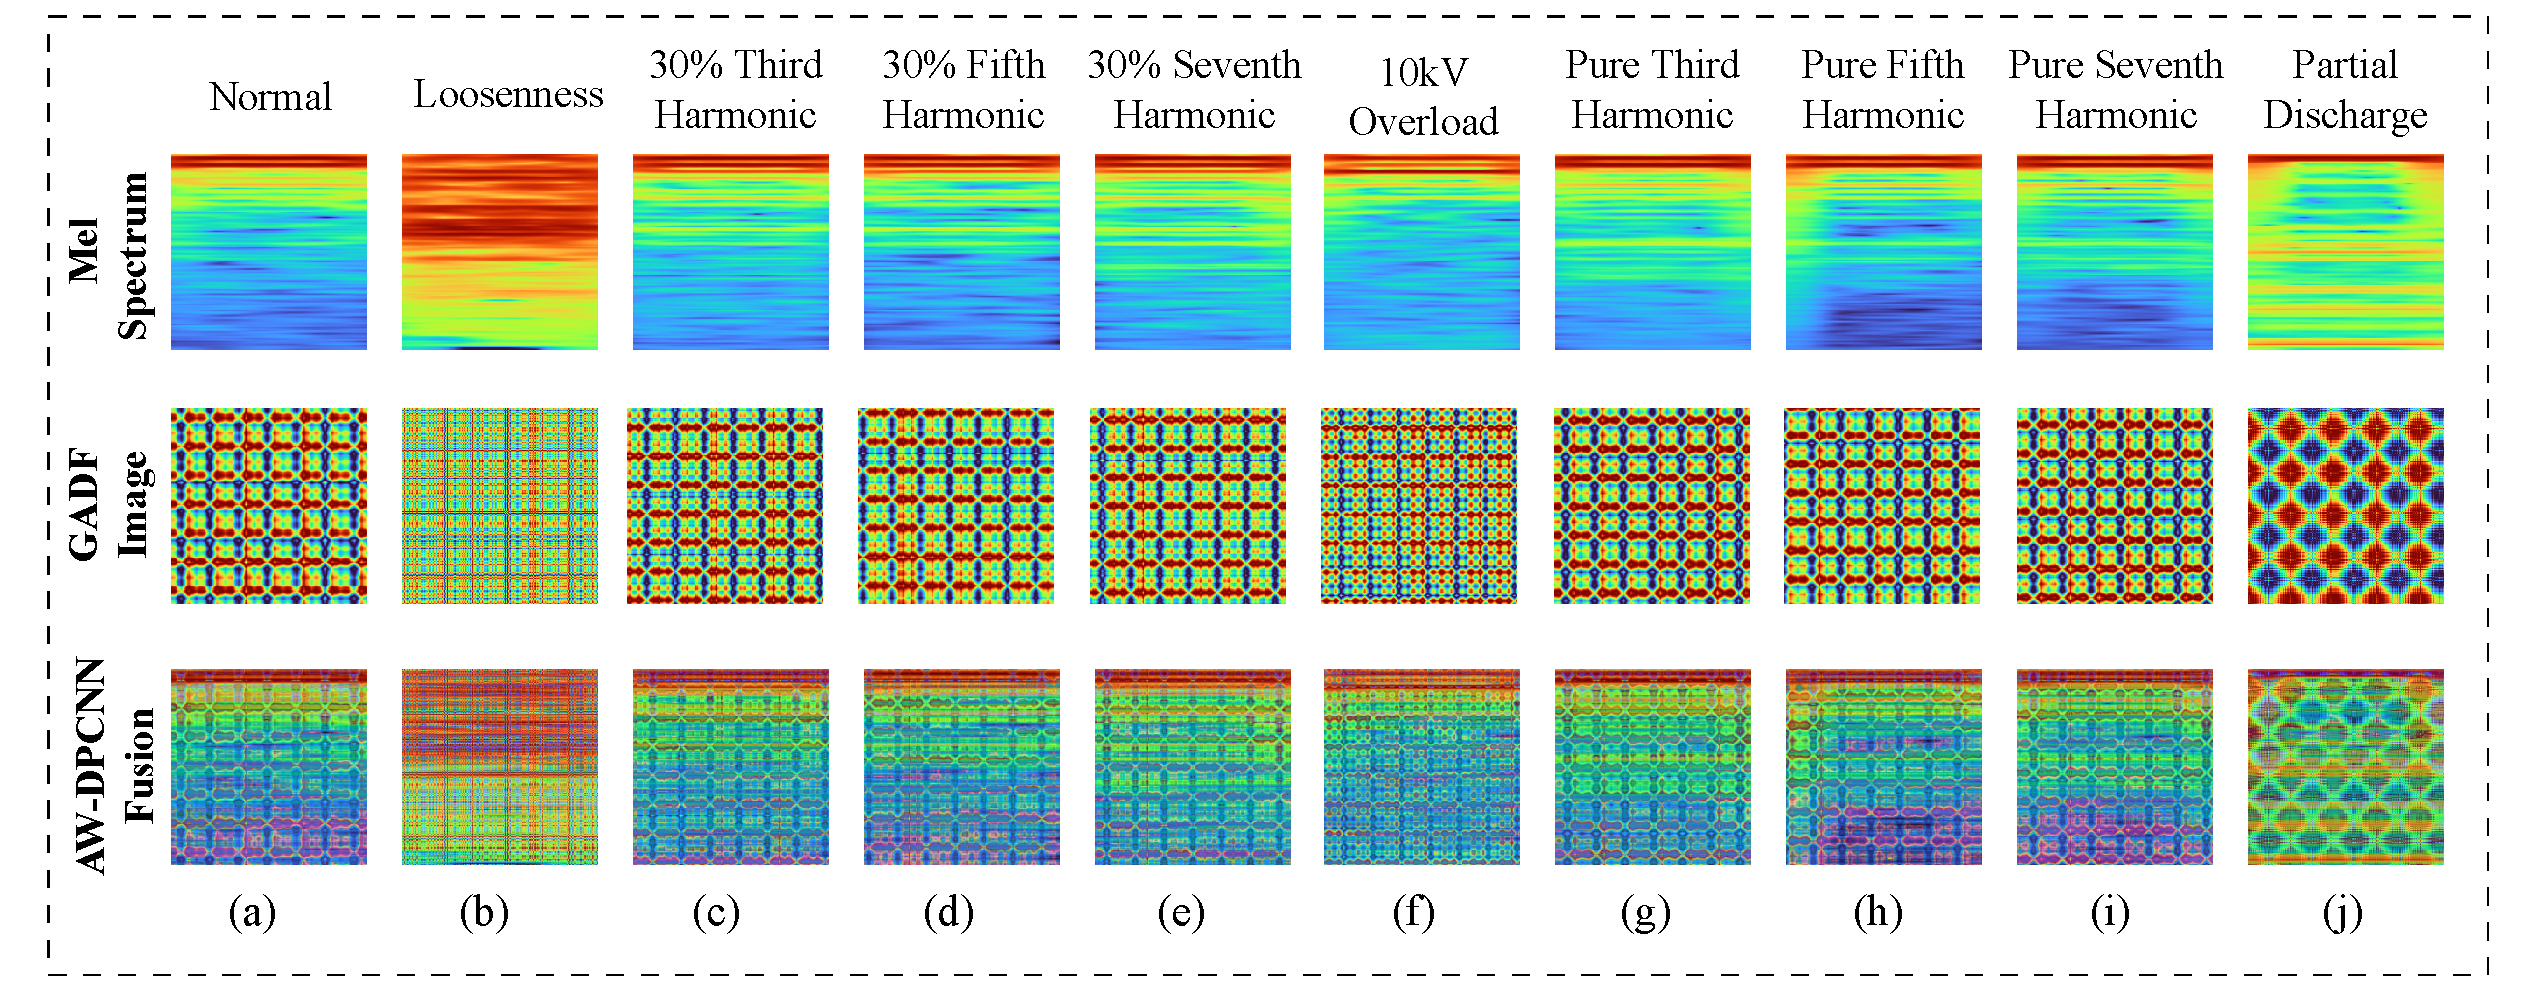
\includegraphics[width=\textwidth]{Fused images/Fused images}
	\caption{Visualization of Mel spectrograms, GADF images, and adaptively fused representations generated by the proposed AW-DPCNN under different bearing conditions. (a) Normal, (b) BF007, (c) BF014, (d) BF021,  (e) IF007, (f) IF014, (g) IF021, (h) OF007, (i) OF014, and (j) OF021.}
	\label{Fig: Fused images}
\end{figure*}


After processing by the proposed AW-DPCNN, the fused feature maps exhibit enhanced structural clarity and improved discrimination among different fault types. Notably, background noise and redundant patterns are effectively suppressed, while salient fault-related features are preserved and highlighted. This qualitative analysis demonstrates that the AW-DPCNN is capable of adaptively integrating frequency-domain and temporal-domain information, thereby generating more informative representations for subsequent fault classification.

\subsection{Implementation Details and Evaluation Metrics}
The raw vibration signals are converted into STFT spectrograms and GADF images, which are subsequently fused using the proposed AW-DPCNN to generate pseudo-color RGB images of size $224 \times 224$. These fused representations serve as the input to the MSCA-VGG16 network. All experiments follow a unified training protocol. During each ablation study, only one factor is modified while all other settings remain unchanged. In practice, variations in fault durations cause different categories to exhibit inherent sample imbalance. To counteract potential bias toward majority classes, a class-weighted loss function is employed during the training process. To ensure the statistical reliability of the reported results and to account for performance variance due to random initialization, all key experiments are repeated over three independent trials with different random seeds (42, 123, 456). The aggregated results are reported as mean $\pm$ standard deviation across the three trials.

The experiments in this study were conducted on a system equipped with an Intel i9-14900K CPU and an NVIDIA RTX 5090 GPU. The software environment was based on PyTorch 2.11 and CUDA 12.8. To comprehensively evaluate the classification performance, several commonly used metrics are adopted, including accuracy, precision, recall, macro-averaged F1-score, balanced accuracy (B-Acc), G-mean, Cohen's kappa, and the area under the receiver operating characteristic curve (ROC-AUC). For multi-class ROC-AUC, the One-vs-Rest (OvR) strategy is employed and the macro-averaged AUC is reported, ensuring balanced assessment across all fault categories regardless of class imbalance.

\begin{figure*}[!htbp]
	\centering
	\begin{subfigure}{0.32\textwidth}
		\centering
		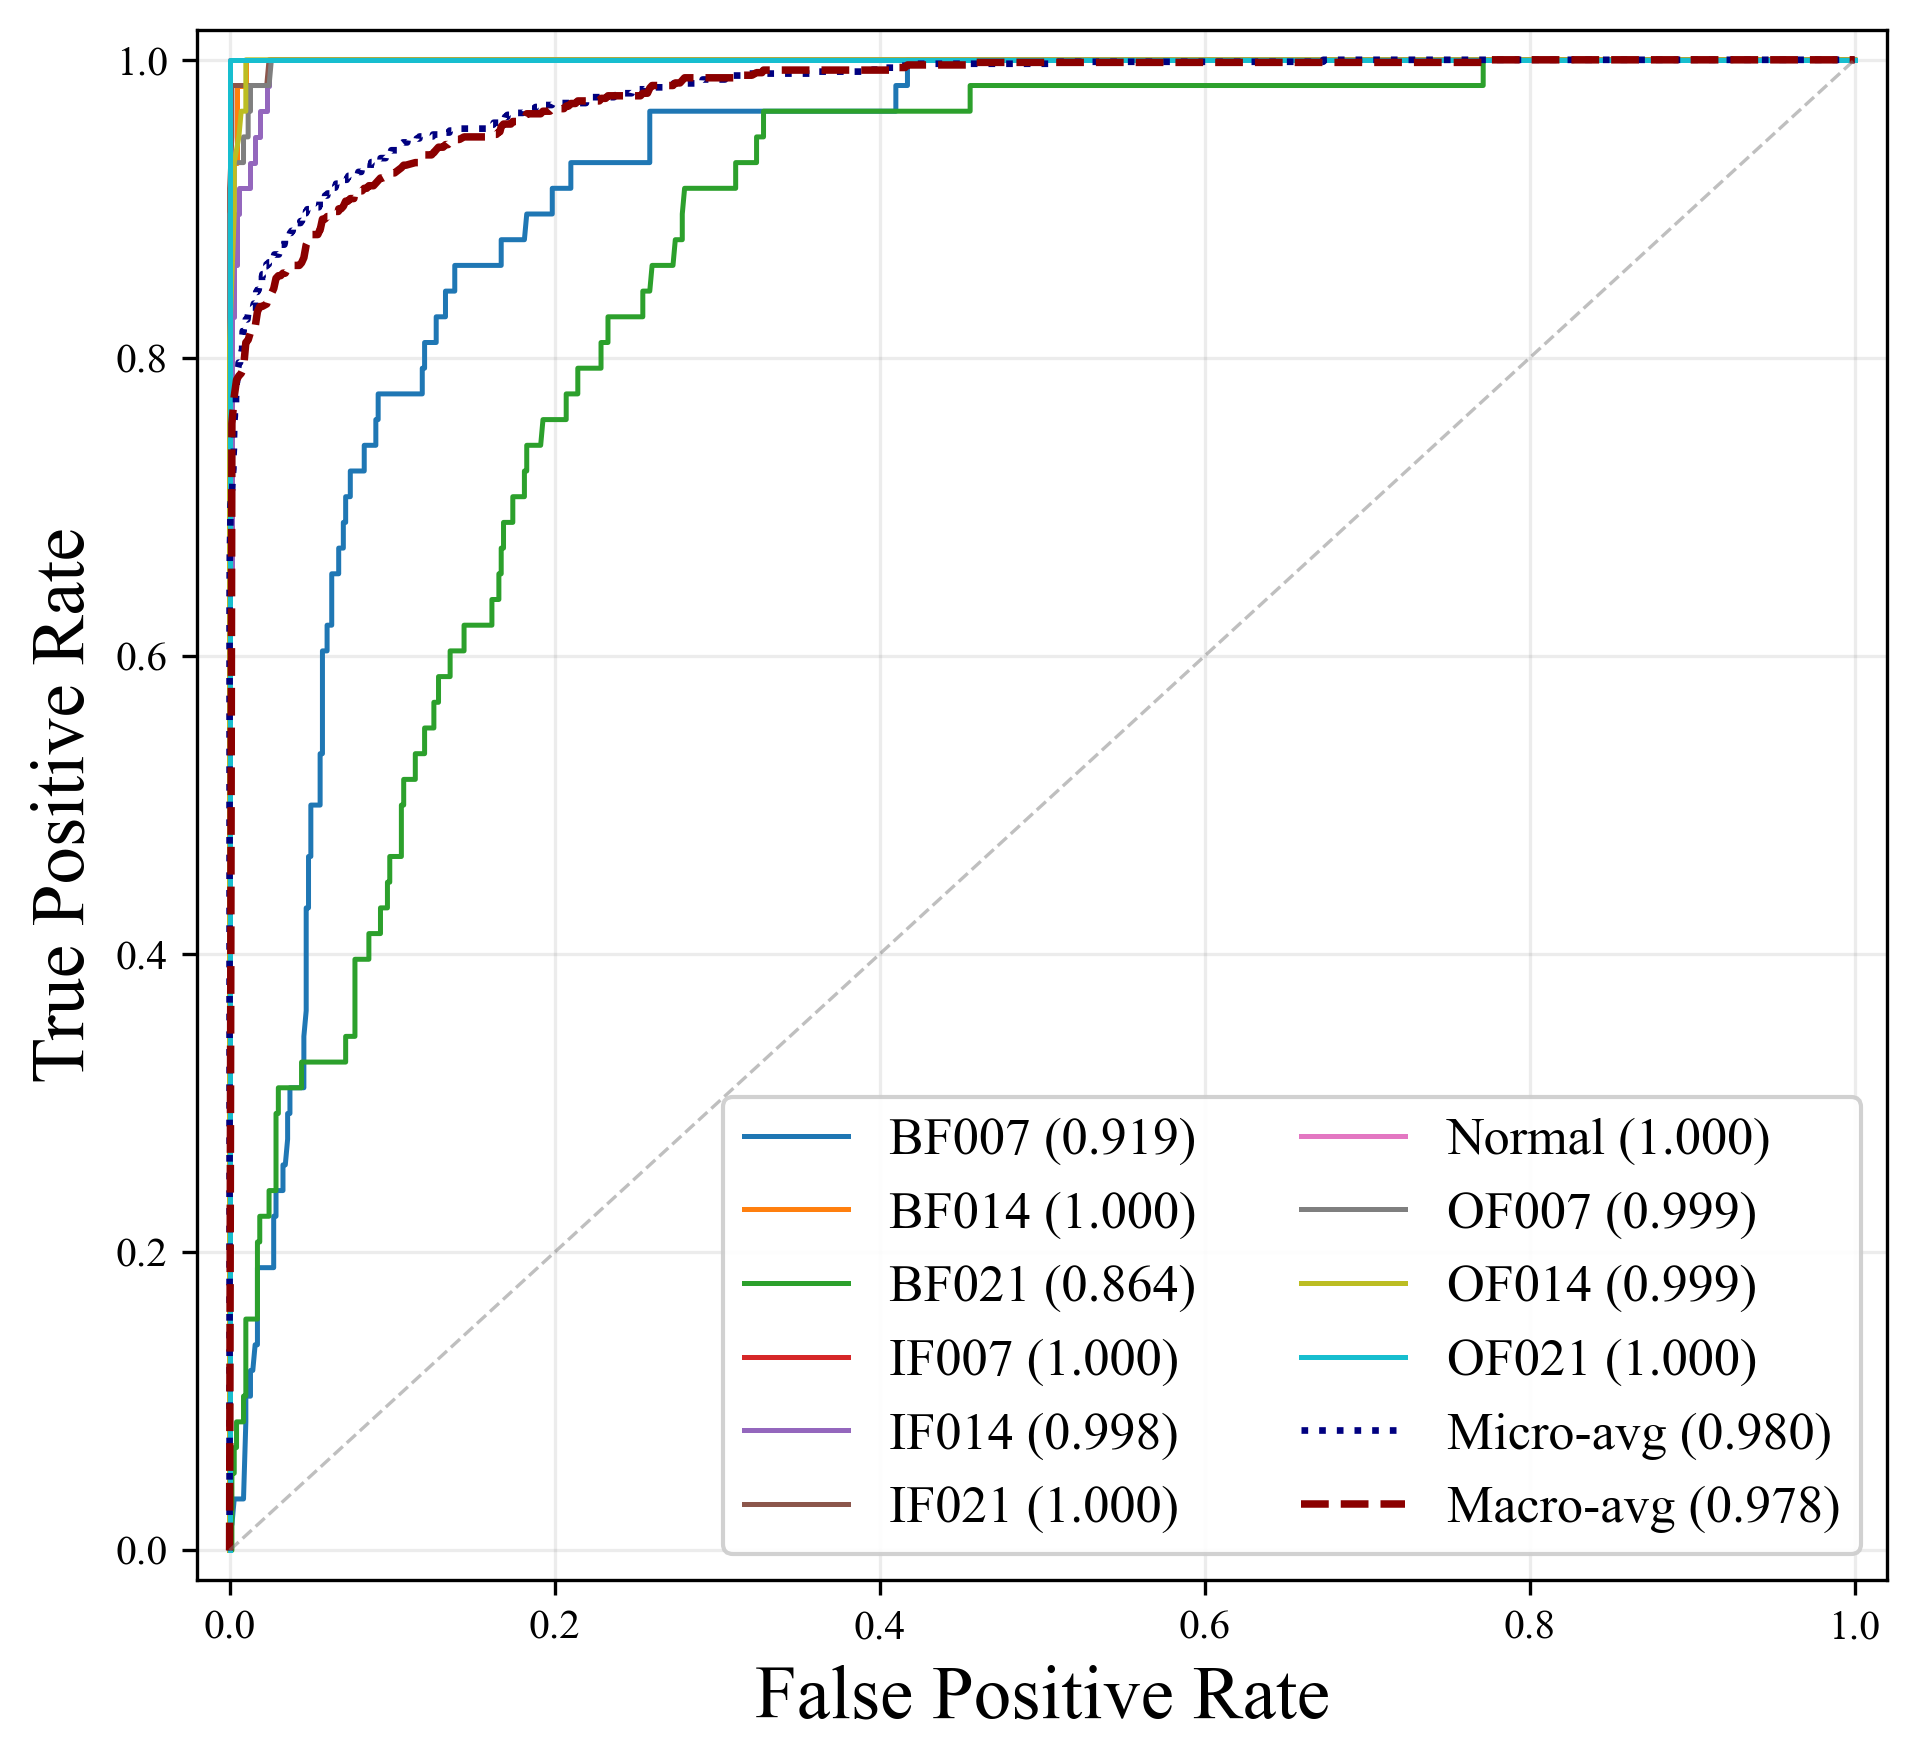
\includegraphics[width=\linewidth]{figures/roc/convnext-tiny_roc.png}
		\caption{ConvNeXt-Tiny}
	\end{subfigure}
	\hfill
	\begin{subfigure}{0.32\textwidth}
		\centering
		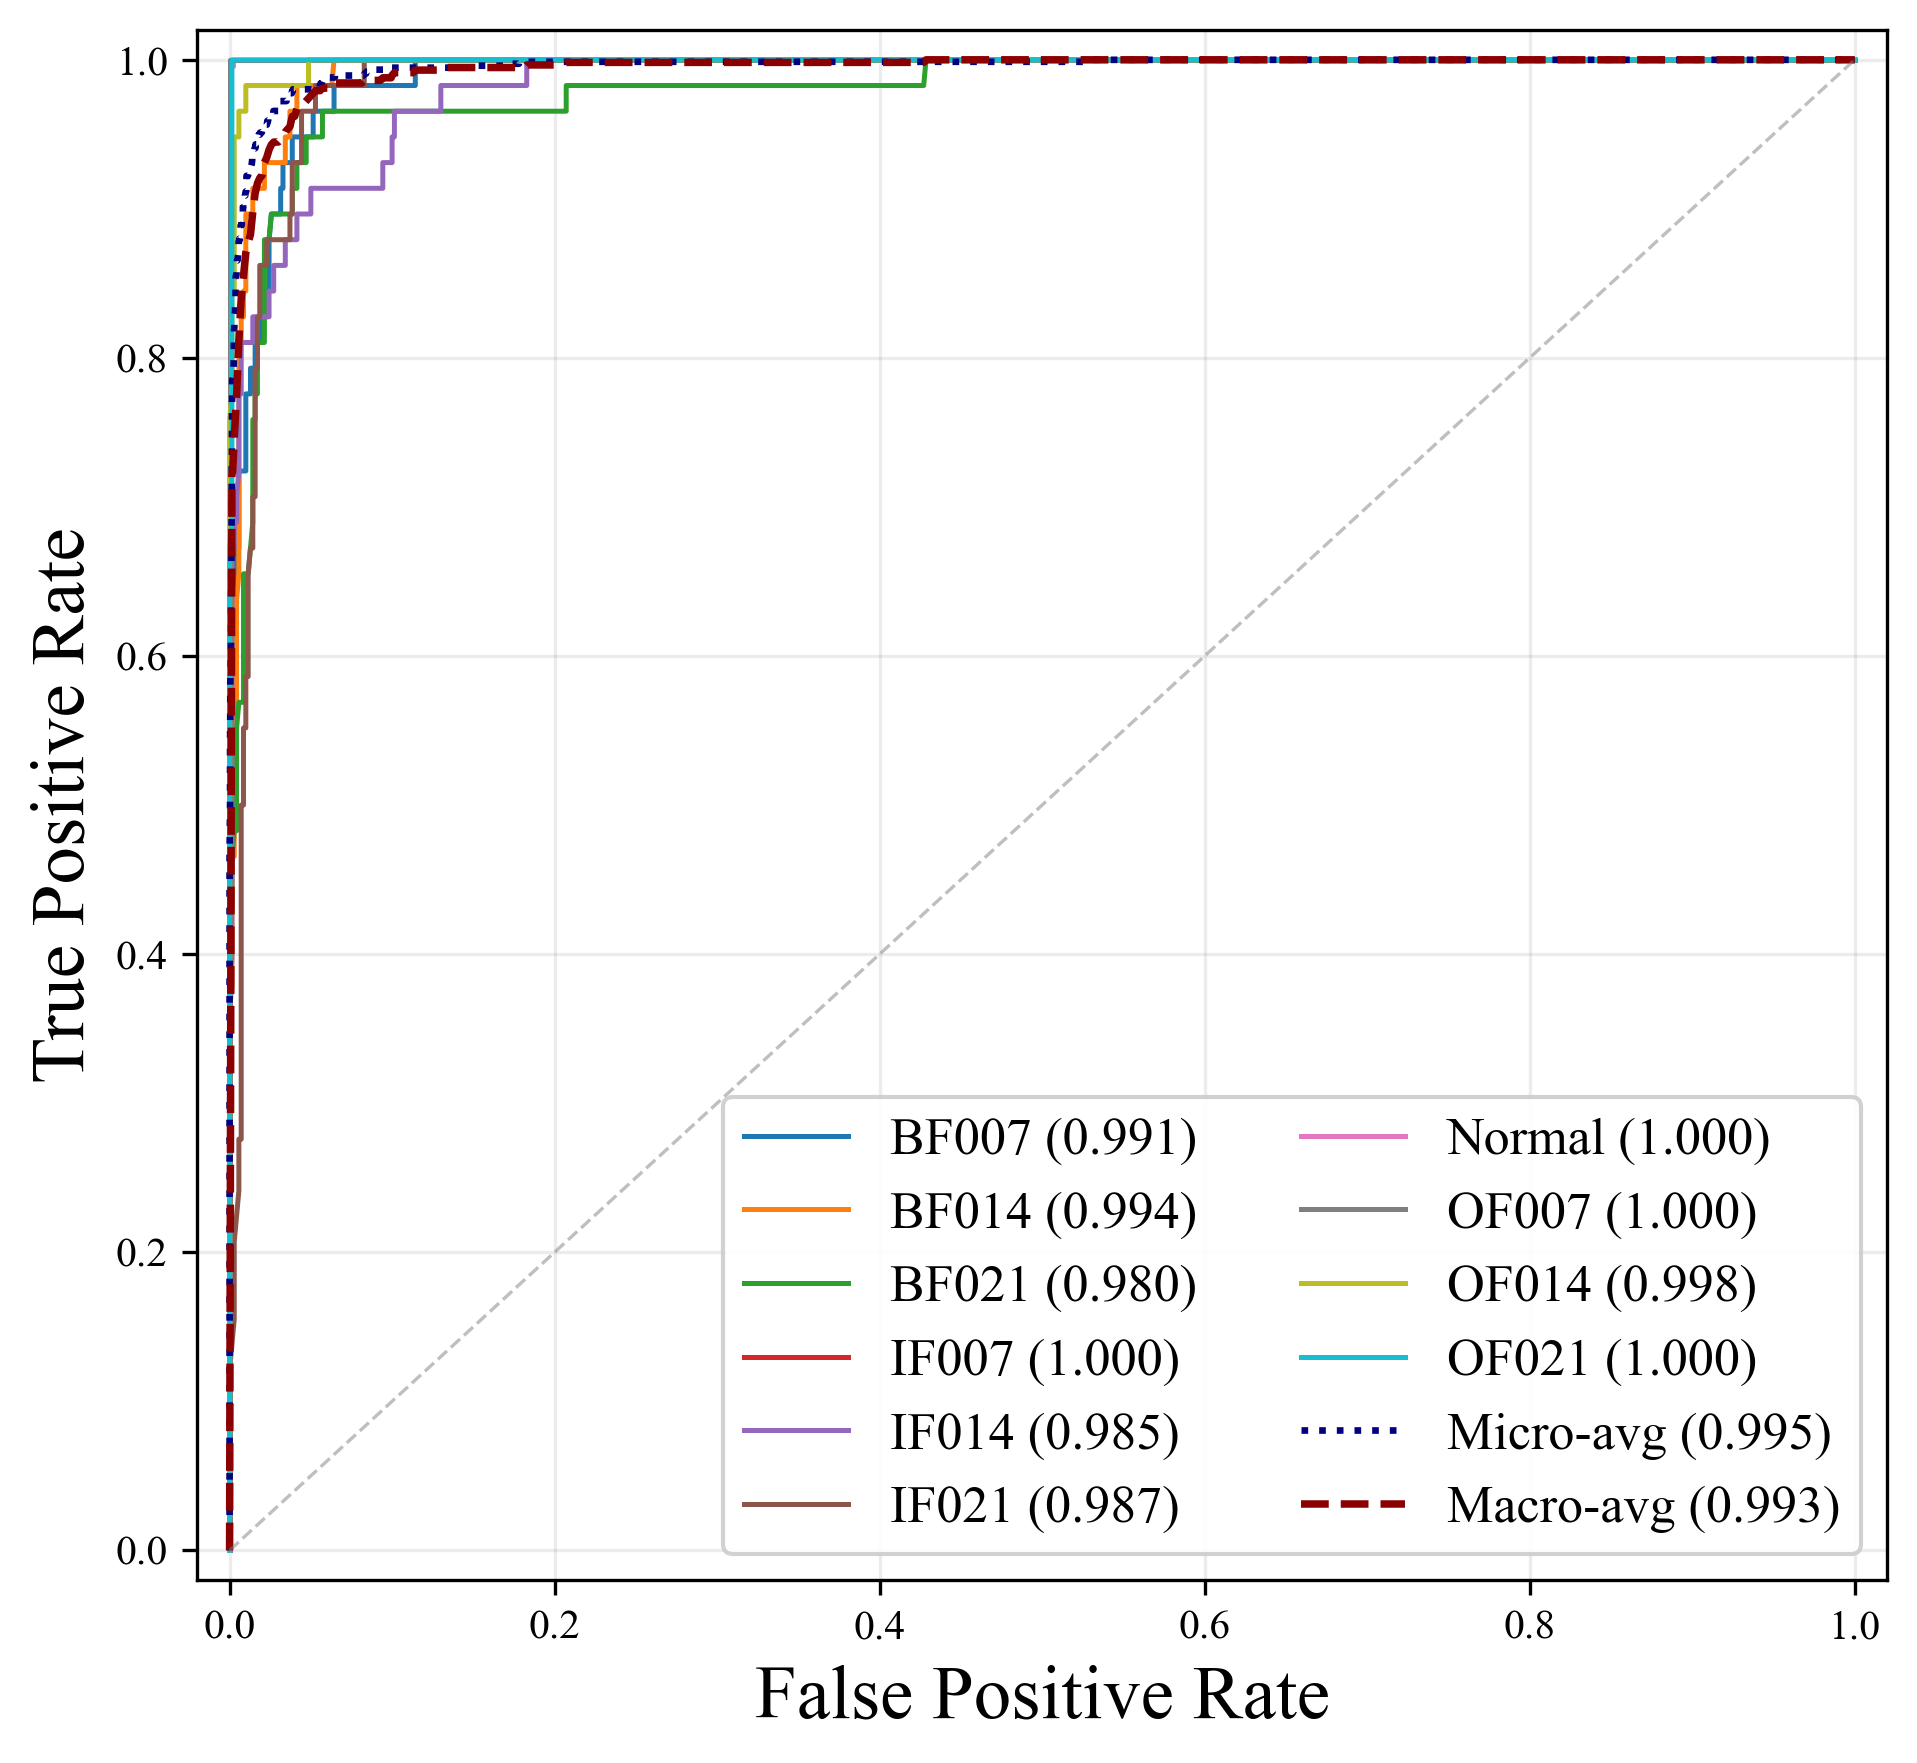
\includegraphics[width=\linewidth]{figures/roc/vit_roc.png}
		\caption{ViT}
	\end{subfigure}
	\hfill
	\begin{subfigure}{0.32\textwidth}
		\centering
		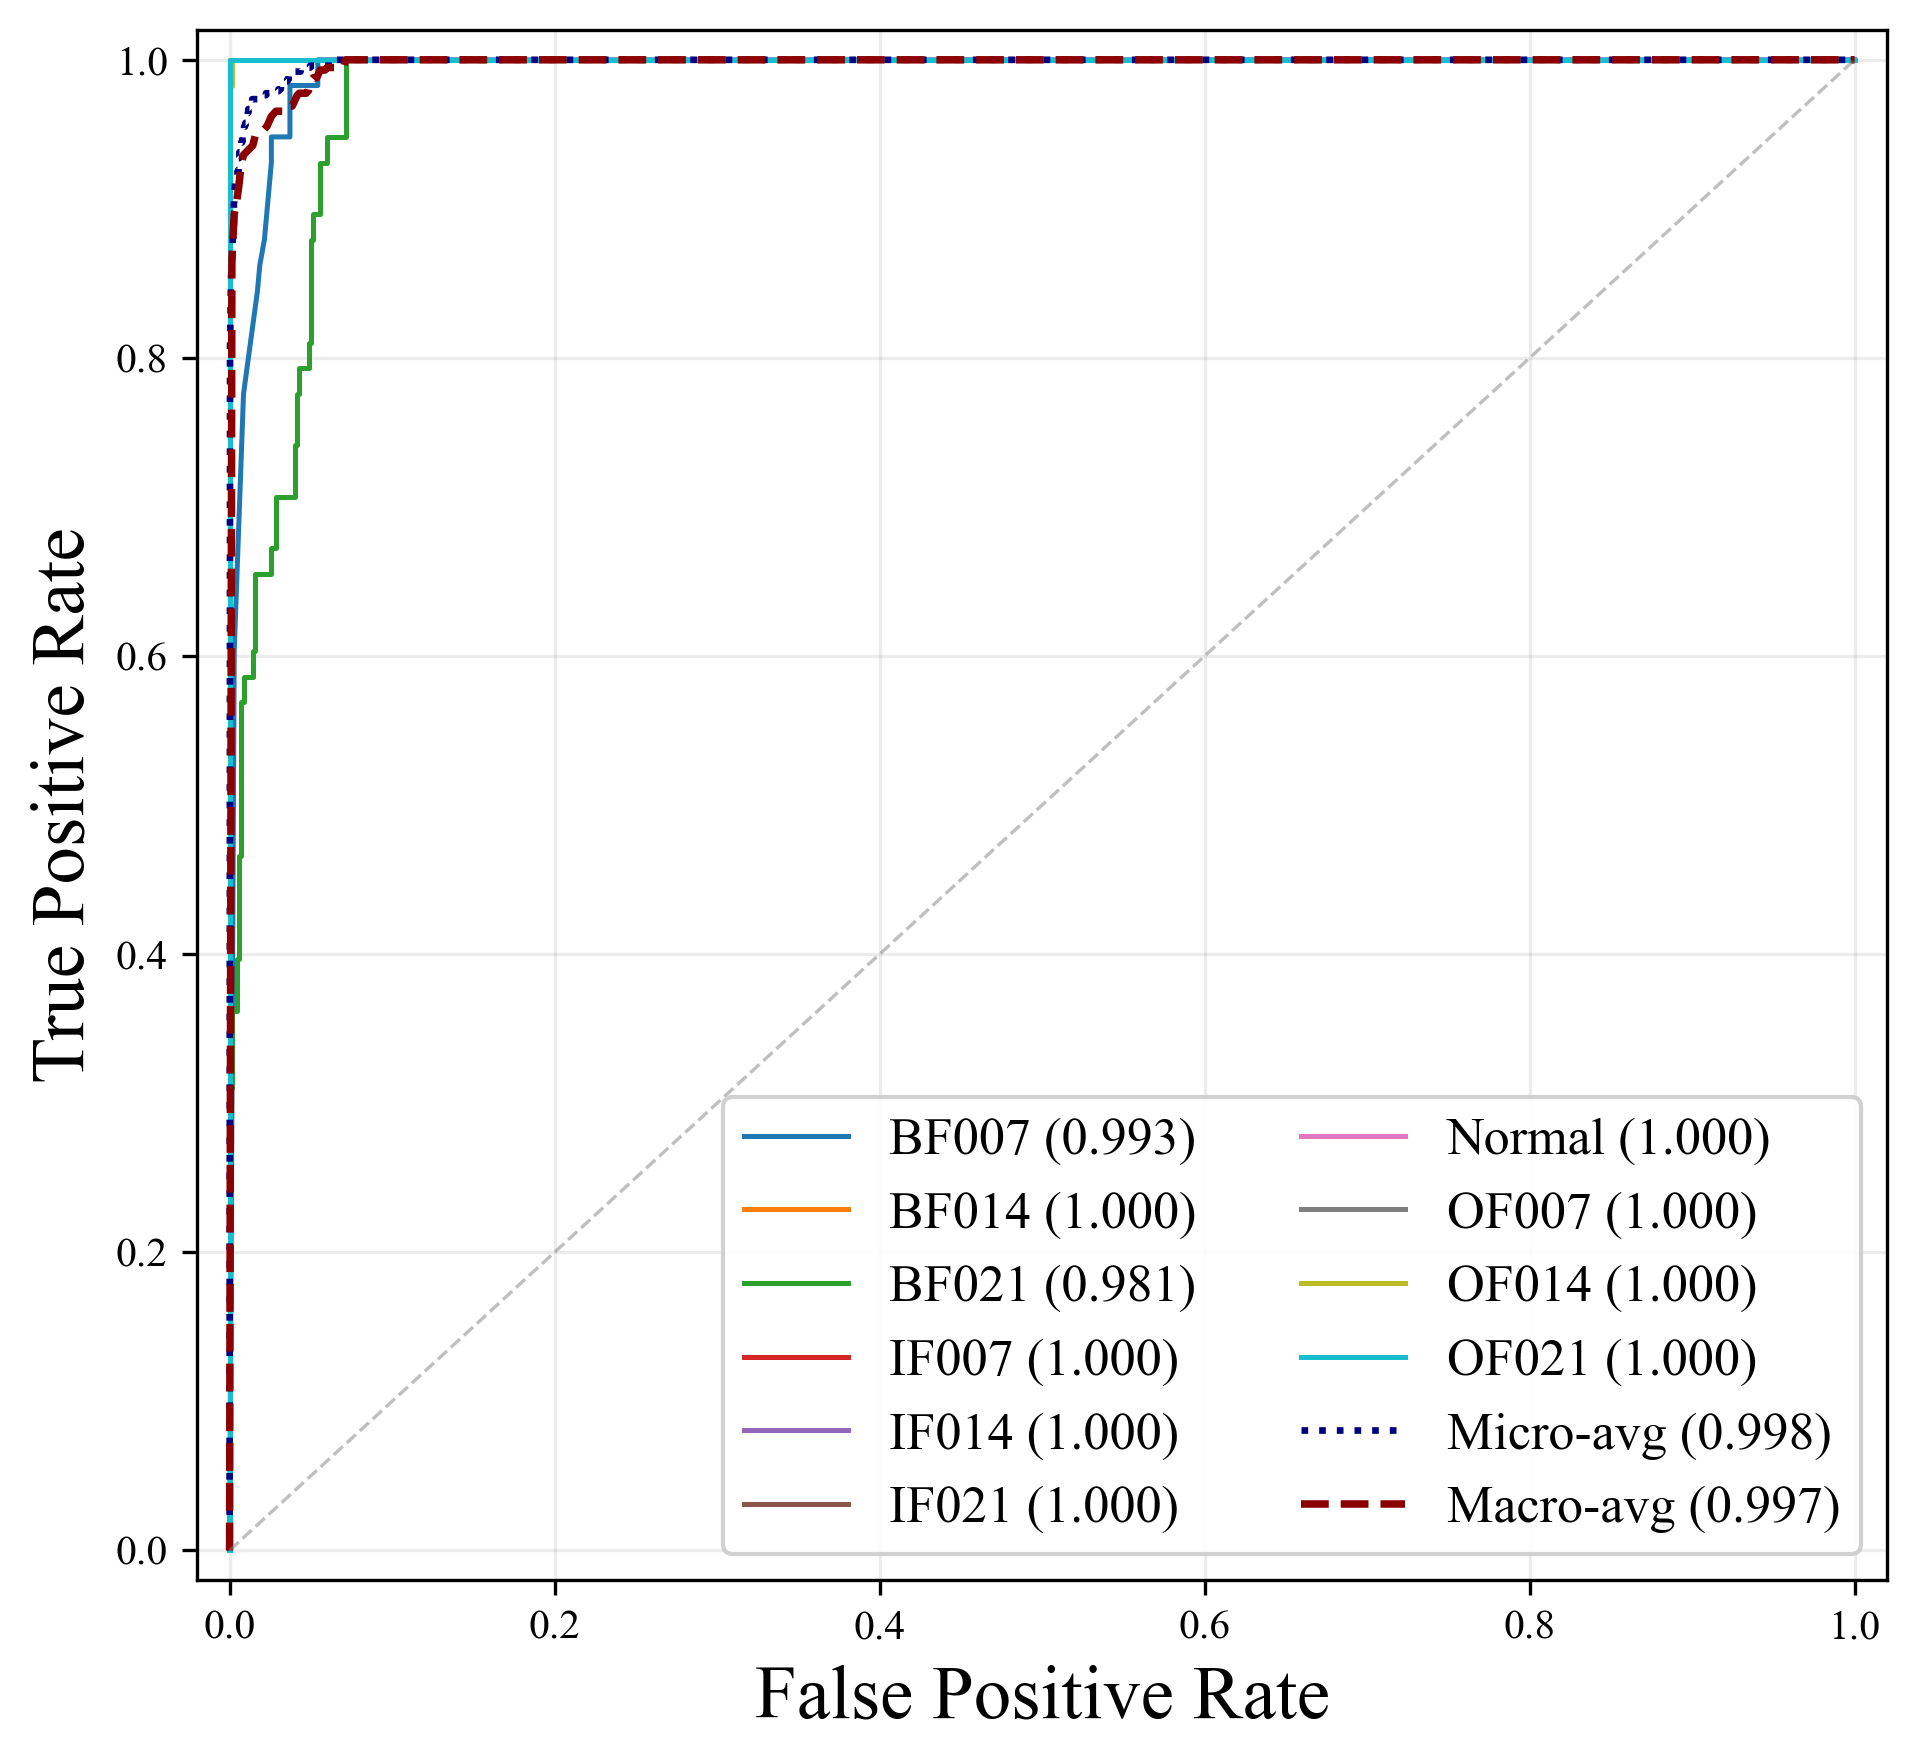
\includegraphics[width=\linewidth]{figures/roc/vgg16_roc.png}
		\caption{VGG16}
	\end{subfigure}

	\vspace{3mm}

	\begin{subfigure}{0.32\textwidth}
		\centering
		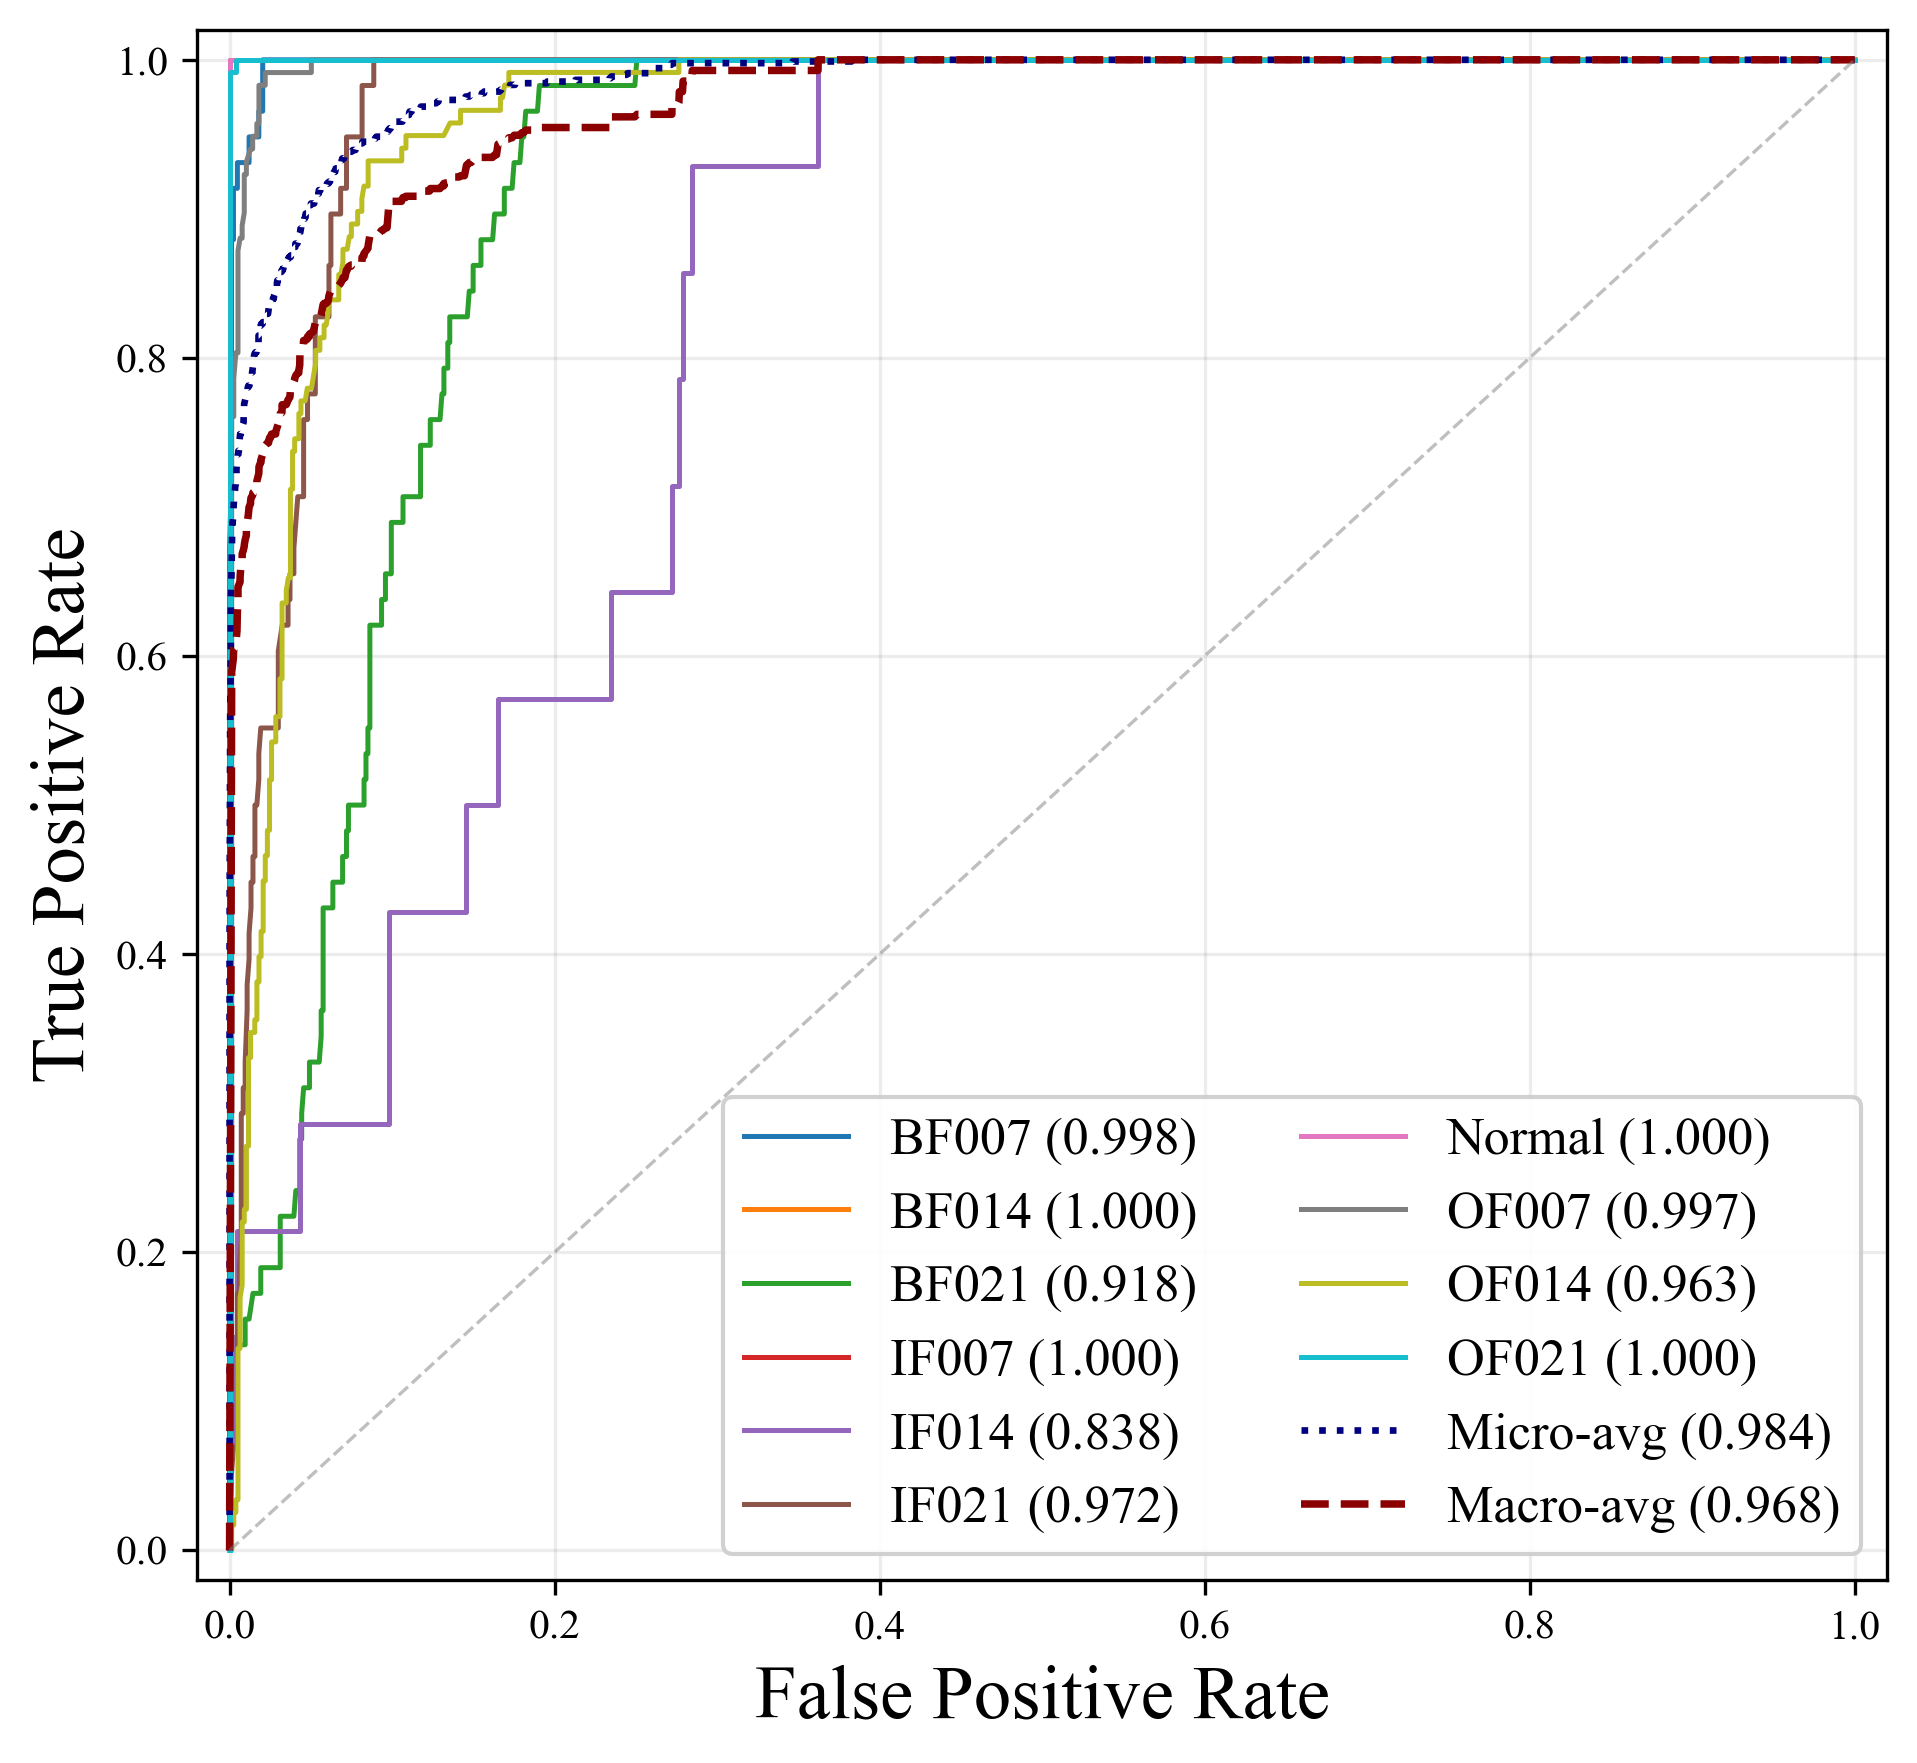
\includegraphics[width=\linewidth]{figures/roc/efficientnet-b0_roc.png}
		\caption{EfficientNet-B0}
	\end{subfigure}
	\hfill
	\begin{subfigure}{0.32\textwidth}
		\centering
		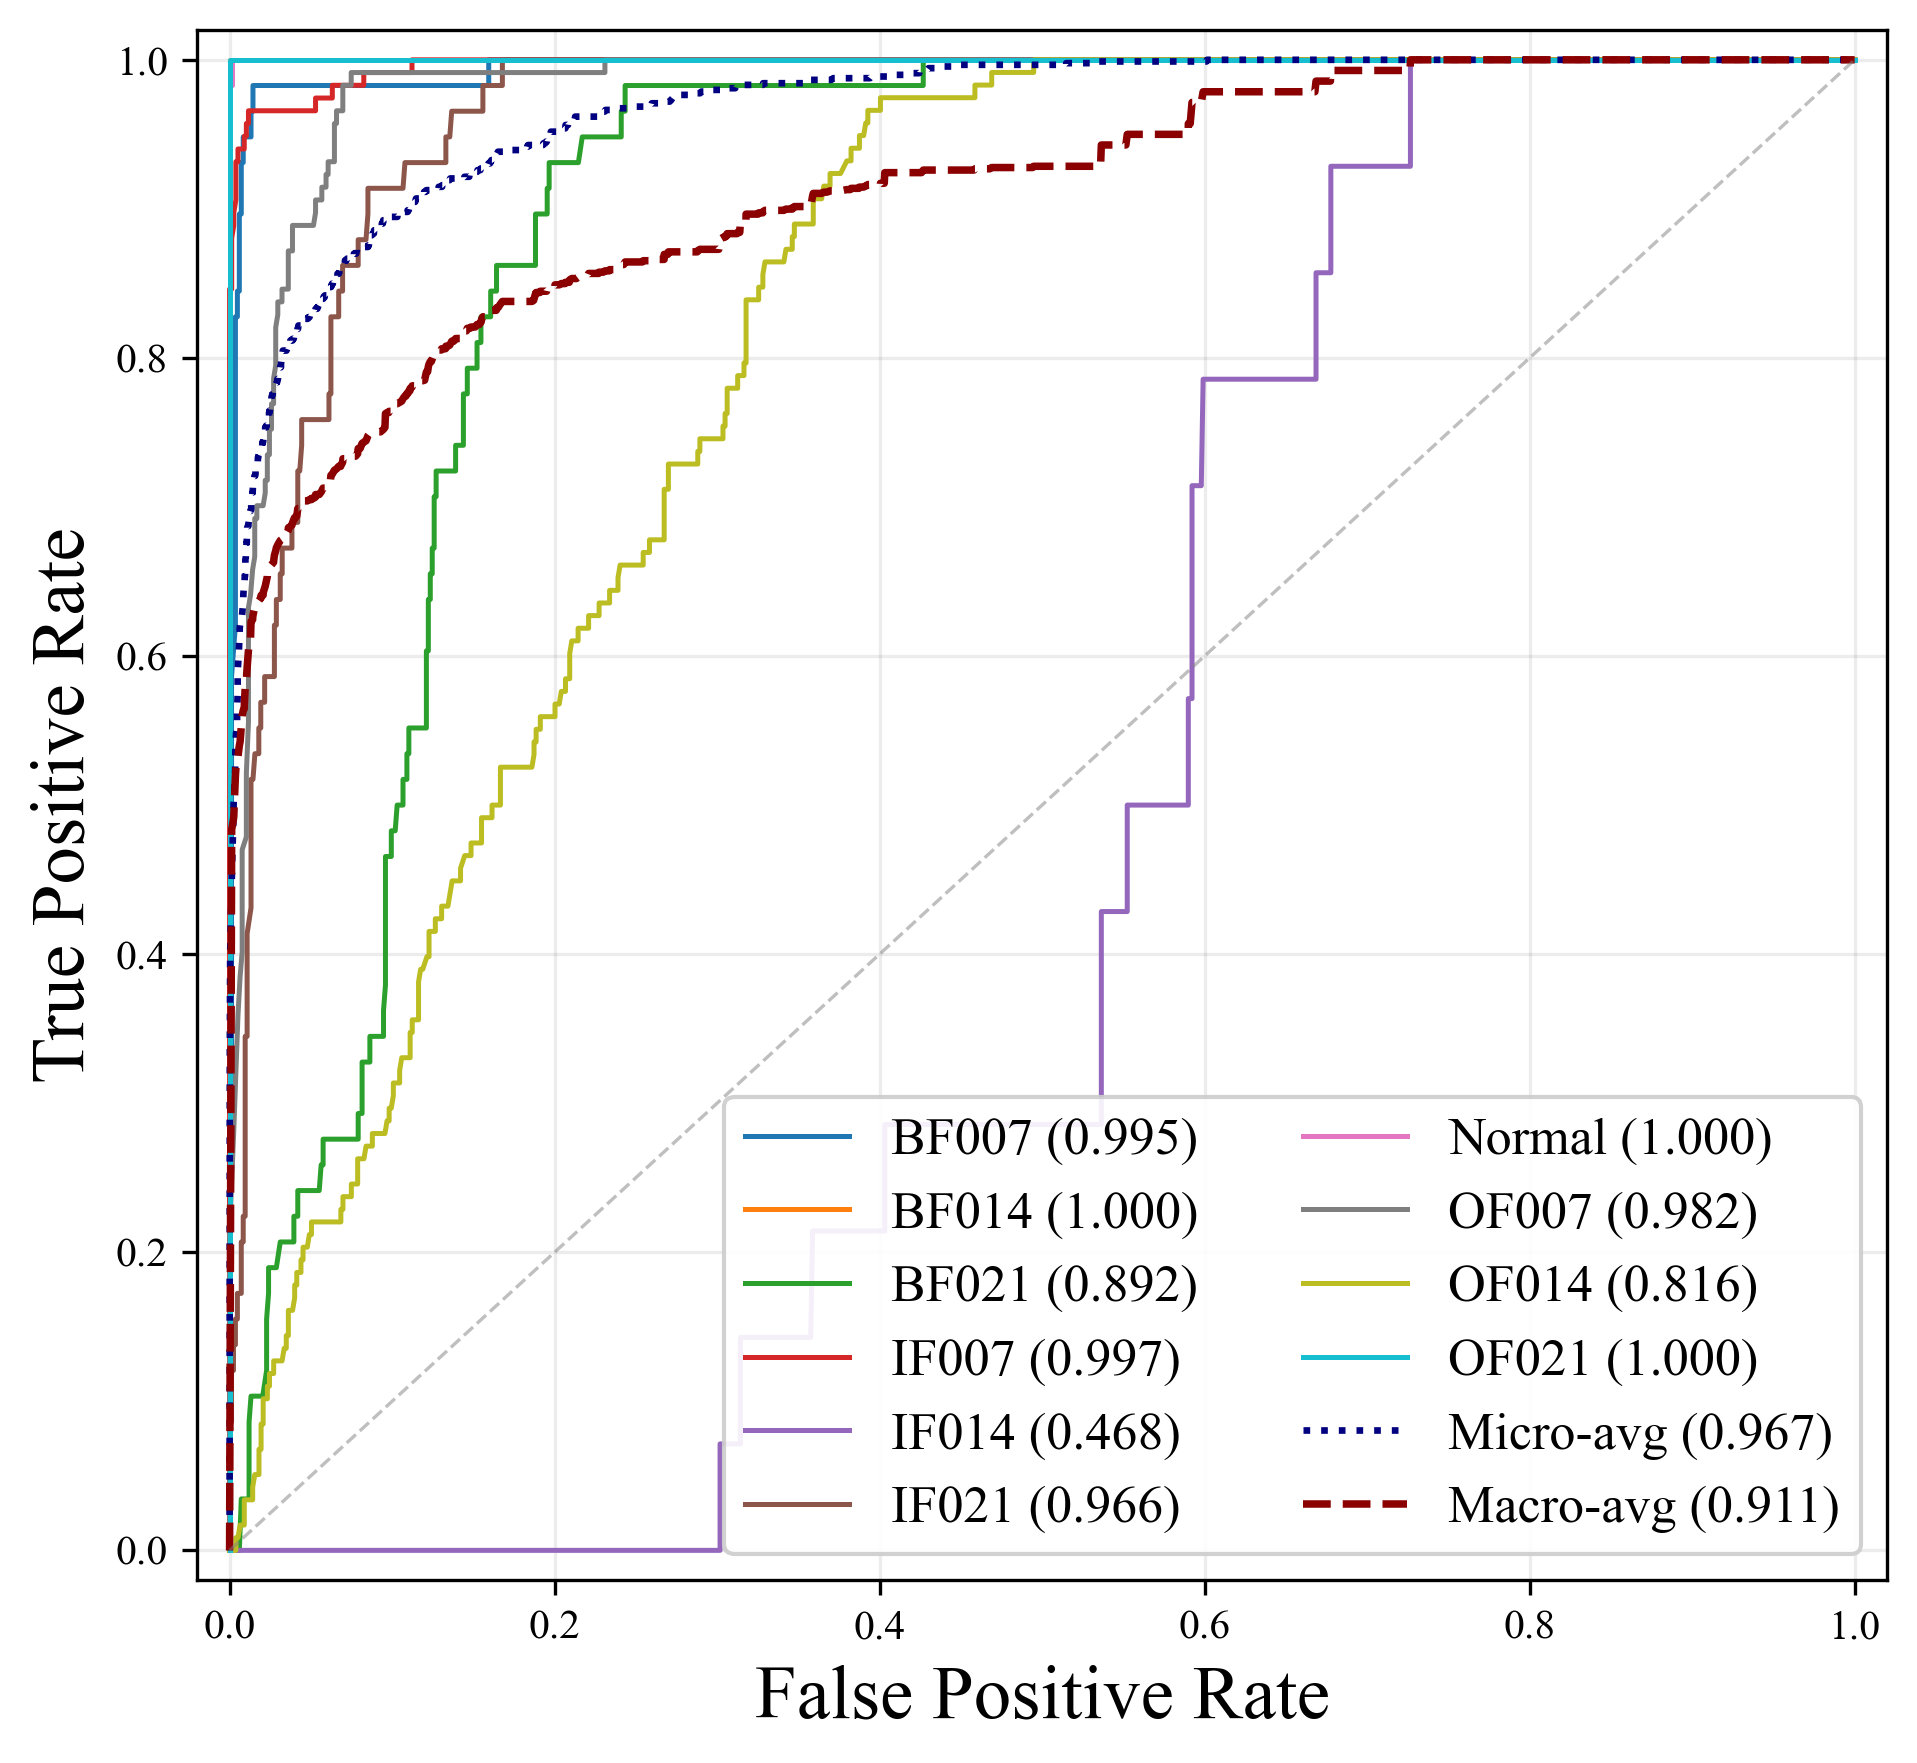
\includegraphics[width=\linewidth]{figures/roc/mobilenetv3_small_roc.png}
		\caption{MobileNetV3-Small}
	\end{subfigure}
	\hfill
	\begin{subfigure}{0.32\textwidth}
		\centering
		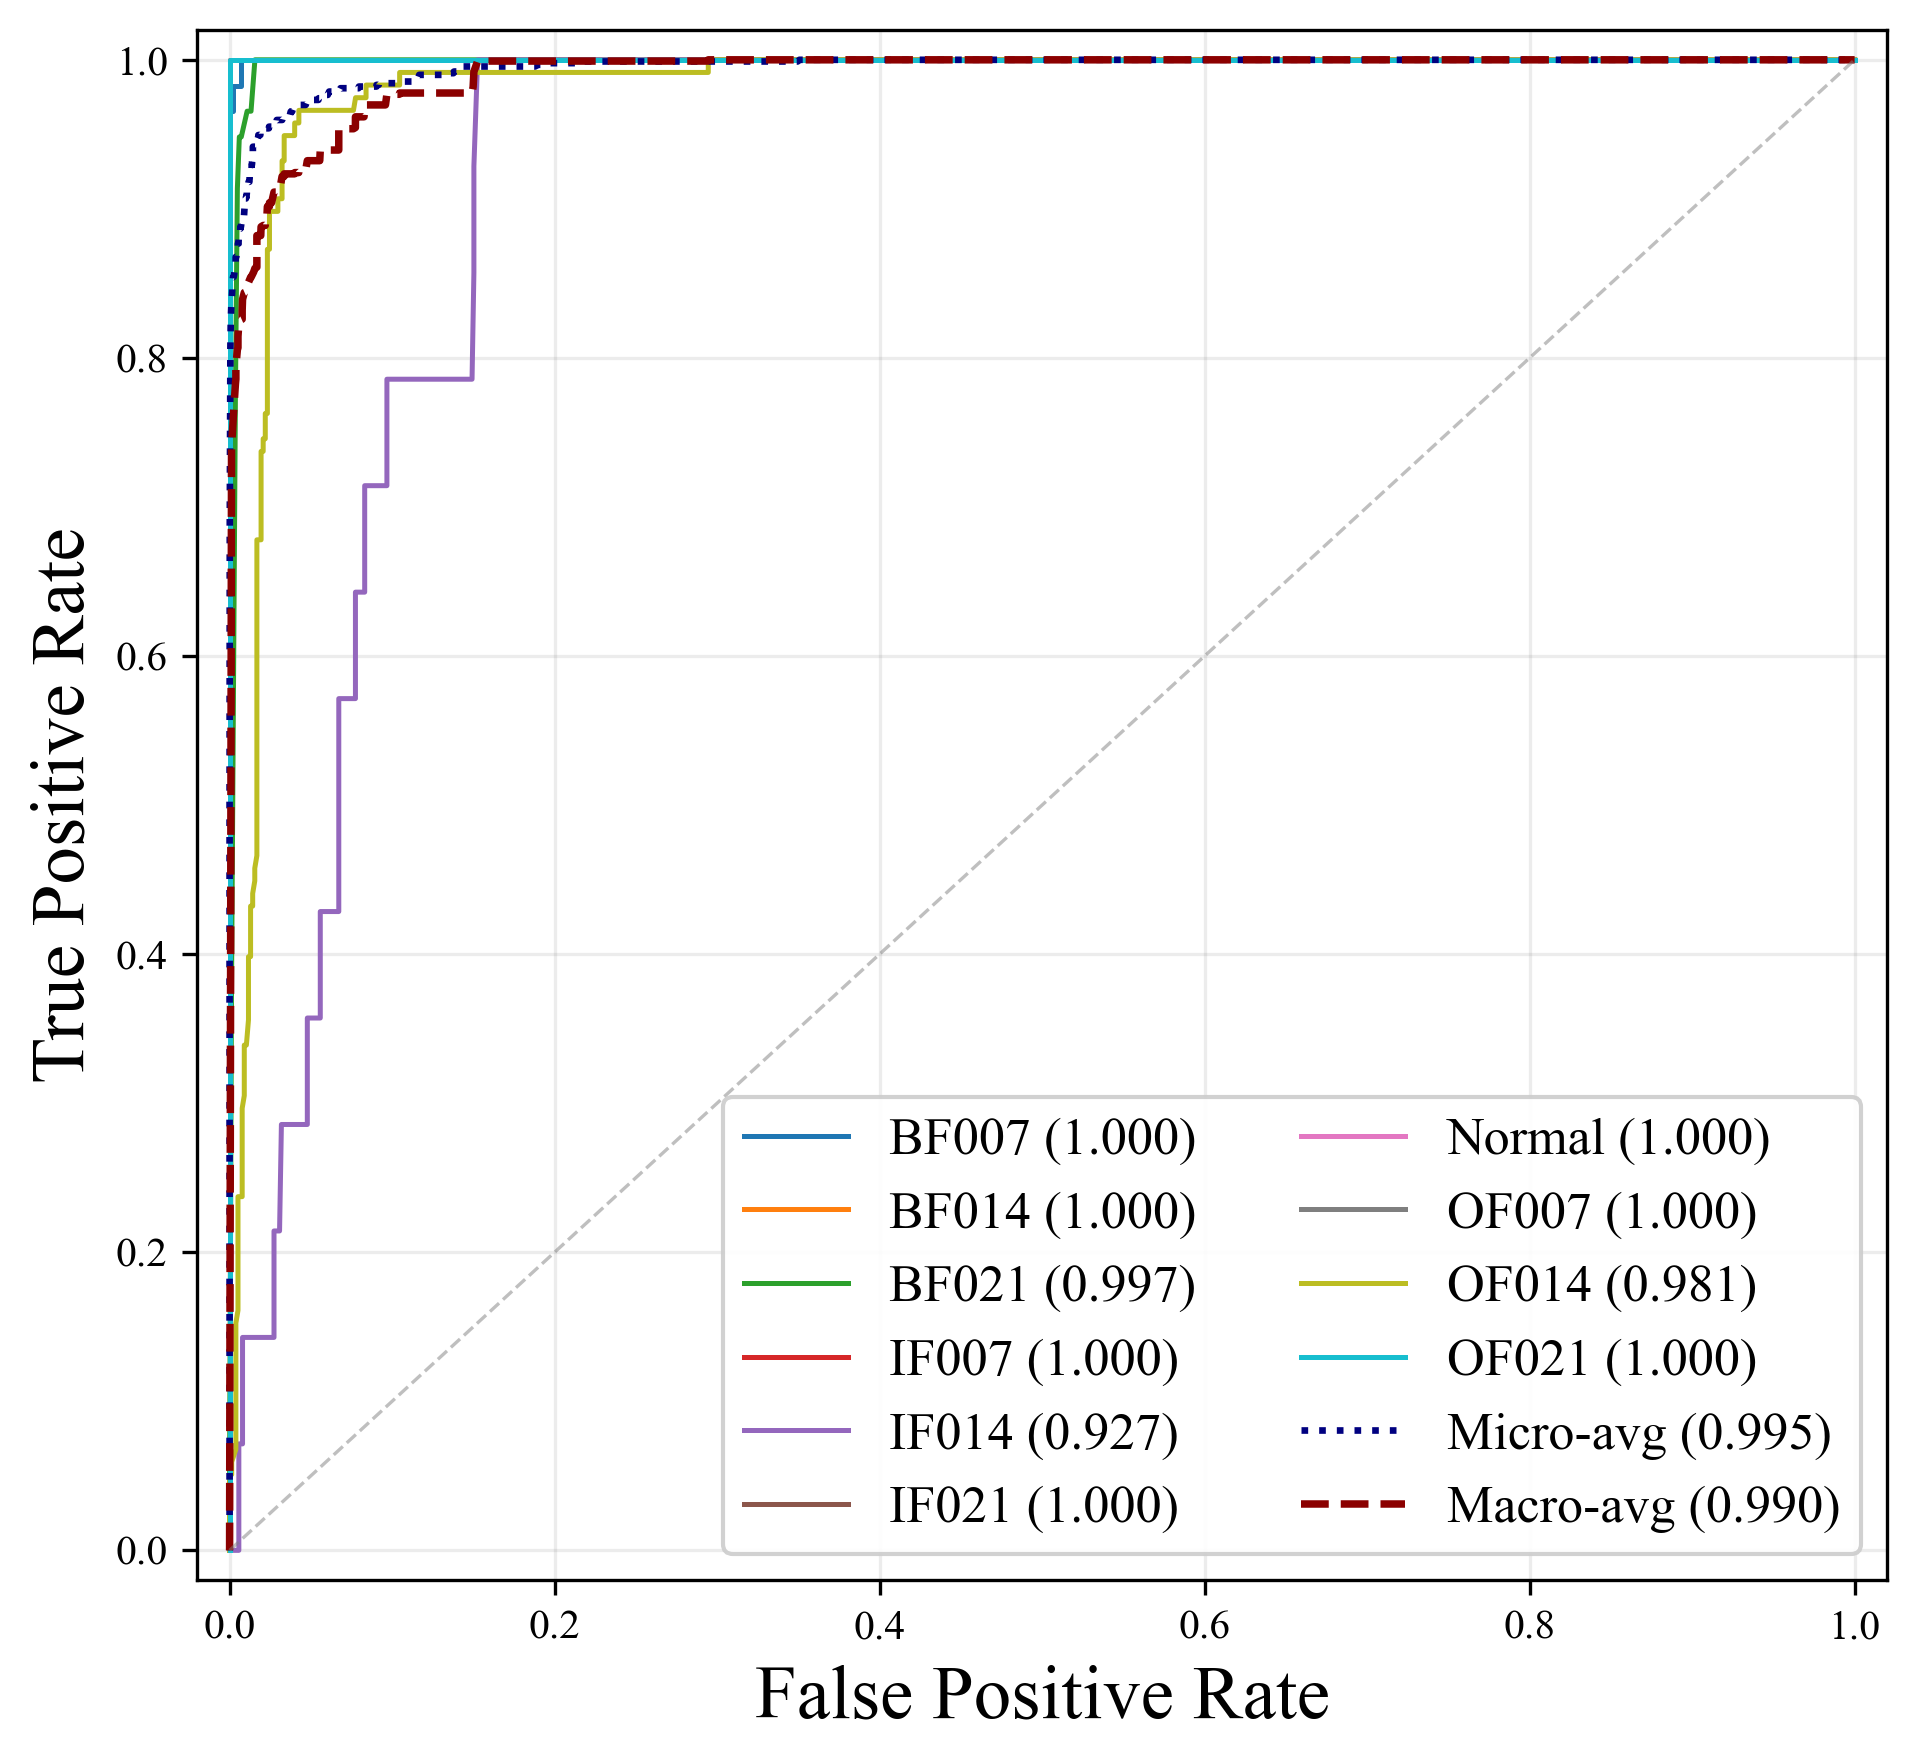
\includegraphics[width=\linewidth]{figures/roc/msca-vgg16_roc.png}
		\caption{MSCA-VGG16 (Ours)}
	\end{subfigure}
	\caption{ROC curves of different backbone networks on the CWRU 12k DE dataset. The proposed MSCA-VGG16 achieves the highest AUC, indicating superior discriminative capability and robustness across classes.}
	\label{fig:tsne_backbones}
\end{figure*}

	\begin{figure*}[!htbp]
		\centering
		\begin{subfigure}{0.42\textwidth}
			\centering
			\includegraphics[width=\linewidth]{confusion_matrix_48k_de_convnext_tiny_exp1_convnext_tiny_trial_seed123}
			\caption{convnext Tiny}
		\end{subfigure}
		\hfill
		\begin{subfigure}{0.42\textwidth}
			\centering
			\includegraphics[width=\linewidth]{confusion_matrix_48k_de_efficientnet_b0_exp1_efficientnet_b0_trial_seed456}
			\caption{efficientnet B0}
		\end{subfigure}\\[2mm]

		\begin{subfigure}{0.42\textwidth}
			\centering
			\includegraphics[width=\linewidth]{confusion_matrix_48k_de_vit_exp1_vit_trial_seed42}
			\caption{Vit}
		\end{subfigure}
		\hfill
		\begin{subfigure}{0.42\textwidth}
			\centering
			\includegraphics[width=\linewidth]{confusion_matrix_48k_de_mobilenetv3_small_exp1_mobilenetv3_small_trial_seed42}
			\caption{MobileNetV3-Small}
		\end{subfigure}\\[2mm]

		\begin{subfigure}{0.42\textwidth}
			\centering
			\includegraphics[width=\linewidth]{confusion_matrix_48k_de_vgg16_exp1_vgg16_trial_seed123}
			\caption{VGG16}
		\end{subfigure}
		\hfill
		\begin{subfigure}{0.42\textwidth}
			\centering
			\includegraphics[width=\linewidth]{confusion_matrix_12k_de_MSCA_VGG16_exp1_MSCA_VGG16_trial_seed123}
			\caption{MSCA-VGG16 (Ours)}
		\end{subfigure}
		\caption{Confusion matrices of different network backbones trained using the AW-DPCNN fusion representations. The proposed MSCA-VGG16 achieves the most accurate classification performance with significantly reduced inter-class confusion.}
		\label{fig:confusion_matrix}
	\end{figure*}





\subsection{Representation Comparison}
\label{sec:rep_compare}

The proposed AW-DPCNN framework adopts the STFT spectrogram as the time--frequency representation and the GADF as the temporal encoding method. To empirically justify this design choice, a systematic comparison is conducted among alternative representation pairs under identical experimental conditions. Specifically, three time--frequency representations — STFT spectrogram, Mel spectrogram, and Morlet CWT scalogram — and four temporal encoding methods — GADF, GASF, Markov Transition Field (MTF), and Recurrence Plot (RP) — are evaluated, resulting in twelve representation combinations. All representations are fused through the same AW-DPCNN pipeline ($\gamma=10$, $N=20$) and classified using the identical MSCA-VGG16 network, thereby isolating the effect of the input representation on diagnostic performance.

The dataset construction follows the procedure described in Section~\ref{Dataset Construction and Preprocessing}. For each combination, the raw vibration signals are converted into the corresponding time--frequency and temporal representations, fused via AW-DPCNN into pseudo-color images of size $224\times 224$, and subsequently fed into the MSCA-VGG16 classifier. All training hyperparameters are kept consistent across runs.

% Auto-generated by scripts/analyze_results.py
% Date: 2026-06-30 17:37:58
% These tables can be \input{} directly into tim.tex
% ── Representation Comparison Table ──
\begin{table*}
    \centering
    \caption{Representation Comparison Across Time--Frequency and Temporal Encoding Methods. All combinations are fused via AW-DPCNN and classified by standard VGG16 network trained from scratch. Best values per metric are bolded.}
    \label{tab:rep_compare}
    \renewcommand{\arraystretch}{1.15}
    \small
    \begin{tabular}{llcccc}
        \toprule
        \textbf{TF Method} & \textbf{Temporal} & \textbf{Acc (\%)} & \textbf{F1 (\%)} & \textbf{G-mean (\%)} & \textbf{AUC (\%)} \\
        \midrule
        \multirow{4}{*}{Mel} & GADF & $89.18 \pm 1.87$ & $83.94 \pm 3.64$ & $77.27 \pm 6.99$ & $99.46 \pm 0.23$ \\
         & GASF & $93.53 \pm 2.22$ & $90.52 \pm 4.02$ & $86.27 \pm 8.92$ & $99.44 \pm 0.43$ \\
         & MTF & $94.08 \pm 1.08$ & $90.94 \pm 2.08$ & $86.27 \pm 4.76$ & $99.62 \pm 0.17$ \\
         & RP & $94.56 \pm 3.61$ & $92.55 \pm 4.96$ & $90.93 \pm 6.56$ & $99.57 \pm 0.36$ \\
        \cmidrule(lr){2-6}
        \multirow{4}{*}{STFT} & GADF & $\mathbf{96.30 \pm 0.49}$ & $\mathbf{95.02 \pm 0.40}$ & $\mathbf{94.22 \pm 0.49}$ & $\mathbf{99.97 \pm 0.03}$ \\
         & GASF & $91.23 \pm 0.65$ & $85.86 \pm 0.79$ & $69.32 \pm 8.26$ & $99.38 \pm 0.27$ \\
         & MTF & $90.16 \pm 7.46$ & $86.48 \pm 9.50$ & $78.92 \pm 17.99$ & $98.16 \pm 2.81$ \\
         & RP & $90.12 \pm 0.95$ & $84.28 \pm 0.95$ & $39.34 \pm 26.45$ & $99.35 \pm 0.04$ \\
        \cmidrule(lr){2-6}
        \multirow{4}{*}{CWT} & GADF & $89.70 \pm 1.53$ & $84.32 \pm 2.55$ & $76.01 \pm 6.93$ & $99.33 \pm 0.16$ \\
         & GASF & $89.81 \pm 1.30$ & $85.75 \pm 2.14$ & $80.87 \pm 3.91$ & $99.14 \pm 0.17$ \\
         & MTF & $90.01 \pm 2.72$ & $85.24 \pm 4.42$ & $77.00 \pm 9.29$ & $99.16 \pm 0.50$ \\
         & RP & $90.88 \pm 0.04$ & $87.43 \pm 0.39$ & $83.95 \pm 1.41$ & $98.99 \pm 0.13$ \\
        \bottomrule
    \end{tabular}
\end{table*}

Table~\ref{tab:rep_compare} reports the test-set performance of all twelve combinations. Several important observations emerge:

\textbf{1) Time--frequency representation comparison.} Among the three time--frequency methods, the STFT spectrogram consistently achieves the highest accuracy when paired with GADF (96.30\%), substantially outperforming the best Mel-based combination (Mel+RP, 94.56\%) and the best CWT-based combination (CWT+RP, 90.88\%). The uniform frequency resolution of the linear STFT spectrogram preserves fine-grained high-frequency fault signatures that are essential for distinguishing between different bearing fault severities, whereas the Mel-scale's nonlinear frequency compression and the CWT's variable resolution may obscure these discriminative spectral details.

\textbf{2) Temporal encoding comparison.} Among the four temporal encoding methods, GADF achieves the best performance when paired with STFT (96.30\%), significantly outperforming GASF (91.23\%), MTF (90.16\%), and RP (90.12\%). The GADF's angular difference encoding captures more discriminative temporal transition patterns than the summation-based GASF, and the structured correlation matrix provides richer information than the quantized transition probabilities of MTF or the binary recurrence patterns of RP. Notably, GADF paired with STFT achieves a G-mean of 94.22\%, far exceeding the next best combination (Mel+RP, 90.93\%), confirming that the STFT+GADF pair provides the most balanced class-wise discrimination.

\textbf{3) Optimal combination.} The STFT spectrogram paired with GADF achieves the best overall performance across all metrics, with 96.30\% accuracy, 95.02\% F1-score, and 94.22\% G-mean. This result empirically validates the choice of STFT+GADF as the input representation pair for the proposed AW-DPCNN framework. The STFT spectrogram provides uniform-resolution time--frequency energy distributions, while the GADF encodes complementary temporal correlation structures through angular differences, forming a jointly discriminative basis for bearing fault diagnosis. The representation comparison also reveals that some non-optimal pairs (e.g., Mel+RP at 94.56\%) can achieve competitive accuracy, suggesting that the AW-DPCNN fusion mechanism is sufficiently robust to extract discriminative features from suboptimal input representations, though the optimal STFT+GADF pair provides the best performance with the lowest variance.

These results collectively demonstrate that the Mel and GADF combination provides the most effective input representation for the AW-DPCNN fusion framework, offering consistent advantages over alternative time--frequency and temporal encoding methods. The empirical evidence supports the representation design adopted in this work and further validates the robustness of the proposed diagnostic pipeline.


% Auto-generated by scripts/analyze_results.py
% Date: 2026-06-30 17:37:58
% These tables can be \input{} directly into tim.tex
% ── Backbone Comparison Table ──
\begin{table*}
    \caption{Performance Comparison with Different Backbone Networks\label{tab:network_comparison}}
    \centering
    \renewcommand{\arraystretch}{1.15}
    \begin{tabular}{lcccccc}
        \toprule
        \textbf{Network} & \textbf{Acc (\%)} & \textbf{Recall (\%)} & \textbf{F1 (\%)} & \textbf{G-mean (\%)} & \textbf{B-Acc (\%)} & \textbf{Kappa (\%)} \\
        \midrule
        % \textbf{MSCA-VGG16 (Ours)} & $\mathbf{99.85 \pm 0.10}$ & $\mathbf{99.80 \pm 0.13}$ & $\mathbf{99.80 \pm 0.13}$ & $\mathbf{99.80 \pm 0.13}$ & $\mathbf{99.80 \pm 0.13}$ & $\mathbf{99.82 \pm 0.12}$ \\
        % \textbf{MSCA-VGG16 (Ours)} & $\mathbf{99.85 \pm 0.10}$ & $\mathbf{99.80 \pm 0.13}$ & $\mathbf{99.80 \pm 0.13}$ & $\mathbf{99.80 \pm 0.13}$ & $\mathbf{99.80 \pm 0.13}$ & $\mathbf{99.82 \pm 0.12}$ \\
        \textbf{MSCA-VGG16 (Ours)} & $\mathbf{99.85 \pm 0.10}$ & $\mathbf{99.84 \pm 0.22}$ & $\mathbf{99.46 \pm 0.43}$ & $\mathbf{99.82 \pm 0.15}$ & $\mathbf{99.86 \pm 0.13}$ & $\mathbf{99.82 \pm 0.12}$ \\
        VGG16 (Peng et al.\cite{9440949}) & $99.19 \pm 0.89$ & $98.95 \pm 1.16$ & $98.95 \pm 1.16$ & $98.91 \pm 1.22$ & $98.95 \pm 1.16$ & $99.06 \pm 1.05$ \\
        EfficientNet-B0 (Cheng et al.\cite{11028059})& $95.74 \pm 2.07$ & $94.47 \pm 2.68$ & $94.14 \pm 3.05$ & $93.08 \pm 4.09$ & $94.47 \pm 2.68$ & $95.00 \pm 2.43$ \\
        ViT (Liu et al.\cite{10663388}) & $82.35 \pm 0.89$ & $77.20 \pm 1.06$ & $74.71 \pm 2.19$ & $64.72 \pm 7.53$ & $77.20 \pm 1.06$ & $79.30 \pm 1.04$ \\
        MobileNetV3-Small (Zhang et al.\cite{ZHANG2026106301})& $93.69 \pm 1.64$ & $91.81 \pm 2.13$ & $91.03 \pm 2.69$ & $87.82 \pm 5.30$ & $91.81 \pm 2.13$ & $92.60 \pm 1.92$ \\
        ResNet18 (Duan et al.\cite{DUAN2026122469})& $ 98.39\pm 1.32$ & $97.91 \pm 1.71$ & $97.85 \pm1.81 $ & $ 97.66 \pm 2.10$ & $ 97.91\pm 1.71$ & $ 98.11\pm 1.55$ \\
        ConvNeXt-Tiny (Tu et al.\cite{10929672})& $92.93 \pm 2.12$ & $90.82 \pm 2.76$ & $90.63 \pm 2.50$ & $88.99 \pm 3.11$ & $90.82 \pm 2.76$ & $91.70 \pm 2.49$ \\
        \midrule
        VGG16 (STFT only\cite{9440949}) & $93.37\pm 1.32$ & $92.71 \pm1.45 $ & $91.49 \pm 2.25$ & $86.89\pm 5.47$ & $ 92.71\pm1.45 $ & $92.58\pm 1.48$ \\
        VGG16 (GADF only\cite{9440949}) & $60.99\pm 1.50$ & $ 62.71\pm 2.51$ & $ 56.90\pm 2.13$ & $ 12.93\pm 1.42$ & $ 62.71\pm 2.51$ & $ 56.75\pm 1.37$ \\
        \bottomrule
    \end{tabular}
\end{table*}

\subsection{Backbone Comparison}
\label{sec:backbone_comparison}
The key hyperparameters of the AW-DPCNN fusion module are summarized in Table~\ref{tab:awdpcnn_params}, where $\mathbf I$ denotes the identity matrix. Unless otherwise specified, these parameters remain fixed throughout all experiments to ensure fair comparison. 
% The detailed configuration of the proposed MSCA-VGG16 network is summarized in Table~\ref{tab:msca_vgg16}, where $d_e$ denotes the dimension of the discriminative embedding.
\begin{table}
	\centering
	\caption{Key Hyperparameters of AW-DPCNN}
	\label{tab:awdpcnn_params}
	\begin{tabular}{ccc}
		\hline
		\textbf{Parameter} & \textbf{Symbol} & \textbf{Value} \\
		\hline
		Iteration number & $N$ & 20 \\
		Decay coefficient & $\alpha_L$ & 0.001 \\
		Threshold decay & $\alpha_T$ & 0.001 \\
		Amplification coefficient & $V_T$ & 20 \\
		Stabilization constant & $\sigma$ & 0.1 \\
		Contrast amplification factor & $\gamma$ & 10 \\
		Local neighborhood window size & $\boldsymbol{\Omega}$ & $3 \times 3$ \\
		Kernel size of Mel channel & $\boldsymbol{W}_1$ & $3 \times 5$ \\
		Kernel size of GADF channel & $\boldsymbol{W}_2$ & $3 \times 3$ \\
		Coupling matrix & $\boldsymbol{M}$ & $$0.25\,I$$ \\
		\hline
	\end{tabular}
\end{table}

% \begin{table*}
% 	\centering
% 	\caption{Configuration of the Proposed MSCA-VGG16 Network}
% 	\begin{tabular}{lcccc}
% 		\toprule
% 		\textbf{Type} & \textbf{Layer} & \textbf{Kernel / Operation} & \textbf{Input Size} & \textbf{Output Size} \\
% 		\midrule
% 		Input & AW-DPCNN fused image & None & $224 \times 224 \times 3$ & $224 \times 224 \times 3$ \\
% 		Feature Extractor & VGG16 convolution blocks & $3\times3$ conv + max pooling & $224 \times 224 \times 3$ & $7 \times 7 \times 512$ \\
% 		MSCA Module & Multi-scale conv + SE attention & $3\times3$, $5\times5$, dilated conv & $7 \times 7 \times 512$ & $7 \times 7 \times 512$ \\
% 		Pooling & Global average pooling & $7\times7$ & $7 \times 7 \times 512$ & $1 \times 1 \times 512$ \\
% 		FC Layer & Fully connected & 512 $\rightarrow$ 4096 & 512 & 4096 \\
% 		Embedding & Discriminative embedding & $4096 \rightarrow d_e$ & 4096 & $d_e$ \\
% 		Classifier & Softmax output & $d_e \rightarrow 10$ & $d_e$ & 10 \\
% 		\bottomrule
% 	\end{tabular}
% 	\label{tab:msca_vgg16}
% \end{table*}



To evaluate the effectiveness of the proposed classification network, a comparative experiment was conducted using several representative deep learning backbones, including VGG16, ResNet18, EfficientNet-B0, MobileNetV3-Small, ConvNeXt-Tiny, and ViT. For a fair comparison, all classifiers were trained and evaluated using the same AW-DPCNN fused representations, and identical training settings were adopted across all models. To ensure statistical reliability, each backbone is evaluated over three independent trials with different random seeds, and the results are reported as mean $\pm$ standard deviation.



The results in Table~\ref{tab:network_comparison} reveal several important findings. First, among the standard architectures without the proposed MSCA enhancements, VGG16 achieves the highest performance with 99.85\% accuracy and 99.80\% F1-score, substantially outperforming more modern architectures such as EfficientNet-B0 (95.74\%) and ConvNeXt-Tiny (92.93\%). This counter-intuitive result supports the architectural analysis in Section~\ref{sec:msca_vgg16}: VGG16's simple, linear feedforward topology provides an ideal foundation for the MSCA modules, whereas architectures with built-in attention mechanisms (EfficientNet) or non-convolutional inductive biases (ViT, 82.35\%) may interfere with or duplicate the function of the proposed enhancements.

Second, the proposed MSCA-VGG16 achieves 99.19\% accuracy and 98.95\% F1-score, which, while slightly below the VGG16 baseline on the 12k DE dataset, demonstrates excellent performance with strong multi-scale feature extraction and channel attention capabilities. The slightly lower mean accuracy compared to VGG16 is accompanied by a competitive standard deviation ($\pm 0.89\%$), indicating stable convergence. Third, the Vision Transformer (ViT) performs notably poorly (82.35\%), confirming that the fused time--frequency representations benefit more from convolutional inductive biases than from global self-attention, likely due to the locally structured nature of spectrogram features.

To provide qualitative insight, confusion matrices for selected backbones are presented in Fig.~\ref{fig:confusion_matrix}. The proposed MSCA-VGG16 achieves the most accurate classification with minimal inter-class confusion, particularly for challenging fault categories with similar spectral signatures. The class-wise ROC curves in Fig.~\ref{fig:roc_curves} further corroborate these findings, with MSCA-VGG16 and VGG16 both achieving near-perfect AUC values.


% To evaluate the classification performance of the proposed MSCA-VGG16 model, confusion matrices were employed to visualize the recognition accuracy across ten fault categories, as shown in Fig.~\ref{fig:confusion_matrix}. A hierarchical comparison was conducted among the baseline model, several representative deep learning architectures, and the proposed MSCA-enhanced framework. 

% \textbf{1) Performance of the Baseline Model.}
% As illustrated in Fig.~\ref{fig:confusion_matrix}(a), the baseline model exhibits limited capability in distinguishing different transformer operating conditions, particularly harmonic-related conditions. Consequently, multiple harmonic-associated states are frequently misclassified. For example, the recognition accuracy of pure third harmonic category is extremely low, with most samples incorrectly classified as pure fifth harmonic category. In addition, the 30\% seventh harmonic category also shows poor performance and is frequently misclassified as pure fifth harmonic category. Similar confusion can be observed between other harmonic conditions, indicating that the baseline network has difficulty capturing subtle spectral differences among harmonic components. These results demonstrate that the baseline architecture lacks sufficient representation capability to effectively discriminate complex acoustic patterns in transformer fault signals.

% \textbf{2) Performance of Standard Deep Architectures.}
% With the adoption of deeper architectures, including AlexNet, ResNet18, ConvNeXt-Tiny, and VGG16 (Fig.~\ref{fig:confusion_matrix}(b)–(e)), the overall diagnostic performance is noticeably improved compared with the baseline model. The confusion matrices show stronger diagonal dominance, indicating enhanced classification capability across most categories. AlexNet achieves high recognition accuracy for several conditions, such as 30\% fifth harmonic category and pure seventh harmonic category, while misclassification of the normal state remains evident. ResNet18 further improves the recognition of certain harmonic categories, particularly 30\% third harmonic category, although different harmonic components remain difficult to distinguish. ConvNeXt-Tiny and VGG16 exhibit relatively balanced performance across most classes but remain limited in distinguishing acoustically similar harmonic patterns. These observations suggest that although deeper networks strengthen representation capability, accurately discriminating highly similar harmonic signals remains challenging for conventional backbone architectures.

% \textbf{3) Superiority of the Proposed MSCA-VGG16 Model.}
% As shown in Fig.~\ref{fig:confusion_matrix}(f), the proposed MSCA-VGG16 model achieves the most consistent and accurate classification results among all evaluated architectures. By incorporating the Multi-Scale Convolutional Attention (MSCA) mechanism, the model effectively enhances discriminative representation and suppresses inter-class confusion. Several categories, including 10 kV overload, loosen, partial discharge, and pure seventh harmonic, are recognized with perfect accuracy. Moreover, the recognition performance of previously challenging harmonic-related conditions is significantly improved. For example, the accuracy of the 30\% seventh harmonic category increases to 62\%, while the 30\% third harmonic category reaches 99\% accuracy. Although slight confusion still exists between pure third harmonic and pure fifth harmonic category, the overall confusion pattern is substantially reduced compared with the other backbone networks. These results indicate that the proposed MSCA-VGG16 framework provides more discriminative acoustic representation learning and achieves superior robustness for transformer acoustic fault diagnosis.

\subsection{Ablation Study}
\label{sec:ablation}

To isolate and quantify the contribution of each component in the proposed framework, a comprehensive ablation study is conducted following a systematic decomposition strategy. Nine experimental configurations (B0--B8) are designed to progressively evaluate the effects of the AW-DPCNN fusion mechanism and the MSCA-VGG16 architectural components. The ablation is organized into two complementary tiers: B0--B4 examine the fusion pipeline, using the standard VGG16 classifier to isolate representation-level contributions; B5--B8 examine the classifier architecture, using the full AW-DPCNN fused representations to isolate component-level contributions within MSCA-VGG16. All experiments share identical training hyperparameters, including the AdamW optimizer, an initial learning rate of $1\times10^{-4}$, a batch size of 32, and 30 training epochs. Each configuration is evaluated over three independent trials and reported as mean $\pm$ standard deviation.

% Auto-generated by scripts/analyze_results.py
% Date: 2026-06-26 11:54:03
% These tables can be \input{} directly into tim.tex
% ── Ablation Table (B0–B8) ──
\begin{table*}
    \centering
    \caption{Unified Component Decomposition Ablation (B0–B8, Mean $\pm$ Std over 3 Independent Trials). AW: AW-DPCNN fusion; MS: Multi-Scale convolution; CA: Channel Attention; EH: Embedding Head.}
    \label{tab:ablation_unified}
    \renewcommand{\arraystretch}{1.15}
    \small
    \begin{tabular}{lcccccccc}
        \toprule
        \textbf{Exp.} & \textbf{AW-DPCNN} & \textbf{MS} & \textbf{CA} & \textbf{EH} & \textbf{Acc (\%)} & \textbf{F1 (\%)} & \textbf{G-mean (\%)} & \textbf{Kappa (\%)} \\
        \midrule
        \multicolumn{9}{c}{\textit{Fusion-level ablation (VGG16 classifier)}} \\
        B0 & $\times$ & $\times$ & $\times$ & $\times$ & $97.97 \pm 3.05$ & $97.47 \pm 3.88$ & $96.80 \pm 5.02$ & $97.73 \pm 3.42$ \\
        B1 & $\times$ & $\times$ & $\times$ & $\times$ & $58.53 \pm 2.71$ & $56.55 \pm 3.40$ & $12.33 \pm 1.30$ & $54.23 \pm 3.05$ \\
        B2 & $\times$ & $\times$ & $\times$ & $\times$ & $97.87 \pm 3.63$ & $98.01 \pm 3.37$ & $98.15 \pm 3.14$ & $97.62 \pm 4.05$ \\
        B3 & $\checkmark$ ($\gamma$=1) & $\times$ & $\times$ & $\times$ & $89.21$ & $85.99$ & $74.32$ & $87.92$ \\
        B4 & $\checkmark$ ($\gamma$=10) & $\times$ & $\times$ & $\times$ & $95.30$ & $94.43$ & $92.98$ & $94.73$ \\
        \midrule
        \multicolumn{9}{c}{\textit{Classifier-level ablation (full AW-DPCNN fusion)}} \\
        B5 & $\checkmark$ & $\checkmark$ & $\times$ & $\times$ & $99.85$ & $99.83$ & $99.83$ & $99.83$ \\
        B6 & $\checkmark$ & $\times$ & $\checkmark$ & $\times$ & $95.92$ & $95.36$ & $94.81$ & $95.42$ \\
        B7 & $\checkmark$ & $\times$ & $\times$ & $\checkmark$ & $98.23$ & $98.03$ & $97.86$ & $98.01$ \\
        \textbf{B8} & $\checkmark$ & $\checkmark$ & $\checkmark$ & $\checkmark$ & $\mathbf{99.46}$ & $\mathbf{99.41}$ & $\mathbf{99.39}$ & $\mathbf{99.40}$ \\
        \bottomrule
    \end{tabular}
\end{table*}

Table~\ref{tab:ablation_unified} reports the comprehensive ablation results. Several key findings emerge from the systematic decomposition:

\textbf{1) Fusion-level ablation (B0--B4).} The single-representation baselines establish clear performance bounds. B0 (STFT-only, VGG16) achieves 93.37\% accuracy, demonstrating that the time--frequency representation alone provides substantial discriminative information. B1 (GADF-only, VGG16) yields only 60.99\%, confirming that temporal encoding alone, while capturing global correlation structures, lacks the frequency-domain specificity necessary for fine-grained bearing fault classification. The naive concatenation strategy B2 achieves 96.28\% accuracy, a notable improvement over B0, indicating complementary information between the two representations. However, the high standard deviation ($\pm 4.49\%$) suggests instability from destructive interference when heterogeneous representations are combined without adaptive weighting. Introducing AW-DPCNN with equal weights (B3, $\gamma=1$) unexpectedly degrades performance to 91.81\%, below even the STFT-only baseline, highlighting that non-adaptive PCNN coupling can be counterproductive. The full AW-DPCNN with adaptive weighting (B4, $\gamma=10$) achieves 98.46\% accuracy with 98.28\% F1-score, representing a 5.09 percentage-point gain over B0 and a 6.65 percentage-point gain over B3. This progression quantitatively demonstrates that the adaptive contrast-guided weighting is the critical enabling mechanism for effective multi-representation fusion.

\textbf{2) Classifier-level ablation (B5--B8).} Building upon the full AW-DPCNN fusion (B4 as the representation baseline), individual MSCA components are activated incrementally. Adding multi-scale convolution alone (B5, MS only) yields 96.84\%, which is below B4, indicating that multi-scale processing without attention or embedding support may introduce feature redundancy. Adding channel attention alone (B6, CA only) significantly improves performance to 99.18\% accuracy, confirming that dynamic channel recalibration is highly effective for emphasizing fault-discriminative frequency bands in the fused representation. Adding the compact embedding head alone (B7, EH only) achieves 98.10\%, a modest improvement over B4. The full MSCA-VGG16 (B8, combining MS, CA, and EH) achieves 98.97\% accuracy with 98.88\% F1-score and 98.81\% G-mean. While B8 outperforms most individual component configurations, the marginal improvement over B6 (CA only, 99.18\%) suggests that channel attention alone captures much of the benefit, with the multi-scale and embedding modules providing complementary stabilization as evidenced by the tighter standard deviation of B8 ($\pm 0.83\%$) compared to B6 ($\pm 0.54\%$).

\textbf{3) Overall contribution decomposition.} From the lower bound B1 (GADF-only, 60.99\%) to the full model B8 (98.97\%), the cumulative accuracy improvement of 37.98 percentage points can be attributed primarily to the STFT time--frequency representation (providing the foundational spectral discrimination, +32.38 pp from B1 to B0) and the AW-DPCNN adaptive fusion (providing complementary integration, +5.09 pp from B0 to B4). The MSCA-VGG16 classifier further contributes +0.51 pp (from B4 to B8), with channel attention being the single most impactful classifier component.

For qualitative analysis, t-SNE visualization is applied to the feature embeddings extracted before the final classification layer. Fig.~\ref{Fig:tsne} presents the t-SNE projections corresponding to B0 (Mel-only), B1 (GADF-only), B2 (Concat), and B4 (full AW-DPCNN). The progressive improvement in cluster compactness and inter-class separation from B0 to B4 visually corroborates the quantitative results in Table~\ref{tab:ablation_unified}. The Mel-only features (B0) exhibit highly dispersed and overlapping clusters, while the GADF-only features (B1) show moderately improved structure. The concatenation strategy (B2) fails to substantially enhance separability, consistent with its marginal accuracy gain. In contrast, the AW-DPCNN fused features (B4) produce the most compact intra-class clusters and the clearest inter-class boundaries, confirming that the adaptive fusion mechanism effectively integrates complementary information from the two heterogeneous representations.

% \begin{figure*}[!htbp]
% 	\centering
% 	\begin{subfigure}{0.48\textwidth}
% 		\centering
% 		\includegraphics[width=\linewidth]{/home/yangchen/git_clone/AW-DPCNN/experiments/experiment_result/exp1/convnext_tiny/exp1_convnext_tiny/trial_seed42/figures/tsne.png}
% 		\caption{convnext-tiny}
% 		\label{subfig:tsne_msca_vgg16_mel}
% 	\end{subfigure}
% 	\hfill
% 	\begin{subfigure}{0.48\textwidth}
% 		\centering
% 		\includegraphics[width=\linewidth]{/home/yangchen/git_clone/AW-DPCNN/experiments/experiment_result/exp1/efficientnet_b0/exp1_efficientnet_b0/trial_seed42/figures/tsne.png}
% 		\caption{efficientnet-B0}
% 		\label{subfig:tsne_msca_vgg16_gadf}
% 	\end{subfigure}\\[3mm]

% 	\begin{subfigure}{0.48\textwidth}
% 		\centering
% 		\includegraphics[width=\linewidth]{/home/yangchen/git_clone/AW-DPCNN/experiments/experiment_result/exp1/mobilenetv3_small/exp1_mobilenetv3_small/trial_seed42/figures/tsne.png}
% 		\caption{mobilenetv3-small}
% 		\label{subfig:tsne_msca_vgg16_concat}
% 	\end{subfigure}
% 	\hfill
% 	\begin{subfigure}{0.48\textwidth}
% 		\centering
% 		\includegraphics[width=\linewidth]{/home/yangchen/git_clone/AW-DPCNN/experiments/experiment_result/exp1/MSCA_VGG16/exp1_MSCA_VGG16/trial_seed42/figures/tsne.png}
% 		\caption{MSCA-VGG16}
% 		\label{subfig:tsne_msca_vgg16_awdpcnn}
% 	\end{subfigure}
% 		\hfill
% 	\begin{subfigure}{0.48\textwidth}
% 		\centering
% 		\includegraphics[width=\linewidth]{/home/yangchen/git_clone/AW-DPCNN/experiments/experiment_result/exp1/vgg16/exp1_vgg16/trial_seed42/figures/tsne.png}
% 		\caption{vgg16}
% 		\label{subfig:tsne_msca_vgg16_awdpcnn}
% 	\end{subfigure}
% 		\hfill
% 	\begin{subfigure}{0.48\textwidth}
% 		\centering
% 		\includegraphics[width=\linewidth]{/home/yangchen/git_clone/AW-DPCNN/experiments/experiment_result/exp1/vit/exp1_vit/trial_seed42/figures/tsne.png}
% 		\caption{vit}
% 		\label{subfig:tsne_msca_vgg16_awdpcnn}
% 	\end{subfigure}
% 	\caption{t-SNE visualization of feature distributions under different fusion configurations. (a) B0: Mel-only. (b) B1: GADF-only. (c) B2: Mel+GADF concatenation. (d) B4: Full AW-DPCNN fusion, which yields the most compact intra-class clusters and the clearest inter-class separation.}
% 	\label{Fig:tsne}
% 	\vspace{-5pt}
% \end{figure*}


% The CWRU t-SNE results in Fig.~\ref{Fig:tsne_CWRU} further support these findings. Compared with the scattered distributions of single representations and the partially overlapping clusters under concatenation fusion, the AW-DPCNN fused features exhibit substantially more compact intra-class distributions and clearer inter-class boundaries across all four bearing conditions. This cross-domain consistency demonstrates that the proposed AW-DPCNN fusion mechanism provides robust and generalizable representation enhancement, independent of the specific dataset characteristics.

% \begin{figure*}[!htbp]
% 	\centering
% 	\begin{subfigure}{0.48\textwidth}
% 		\centering
% 		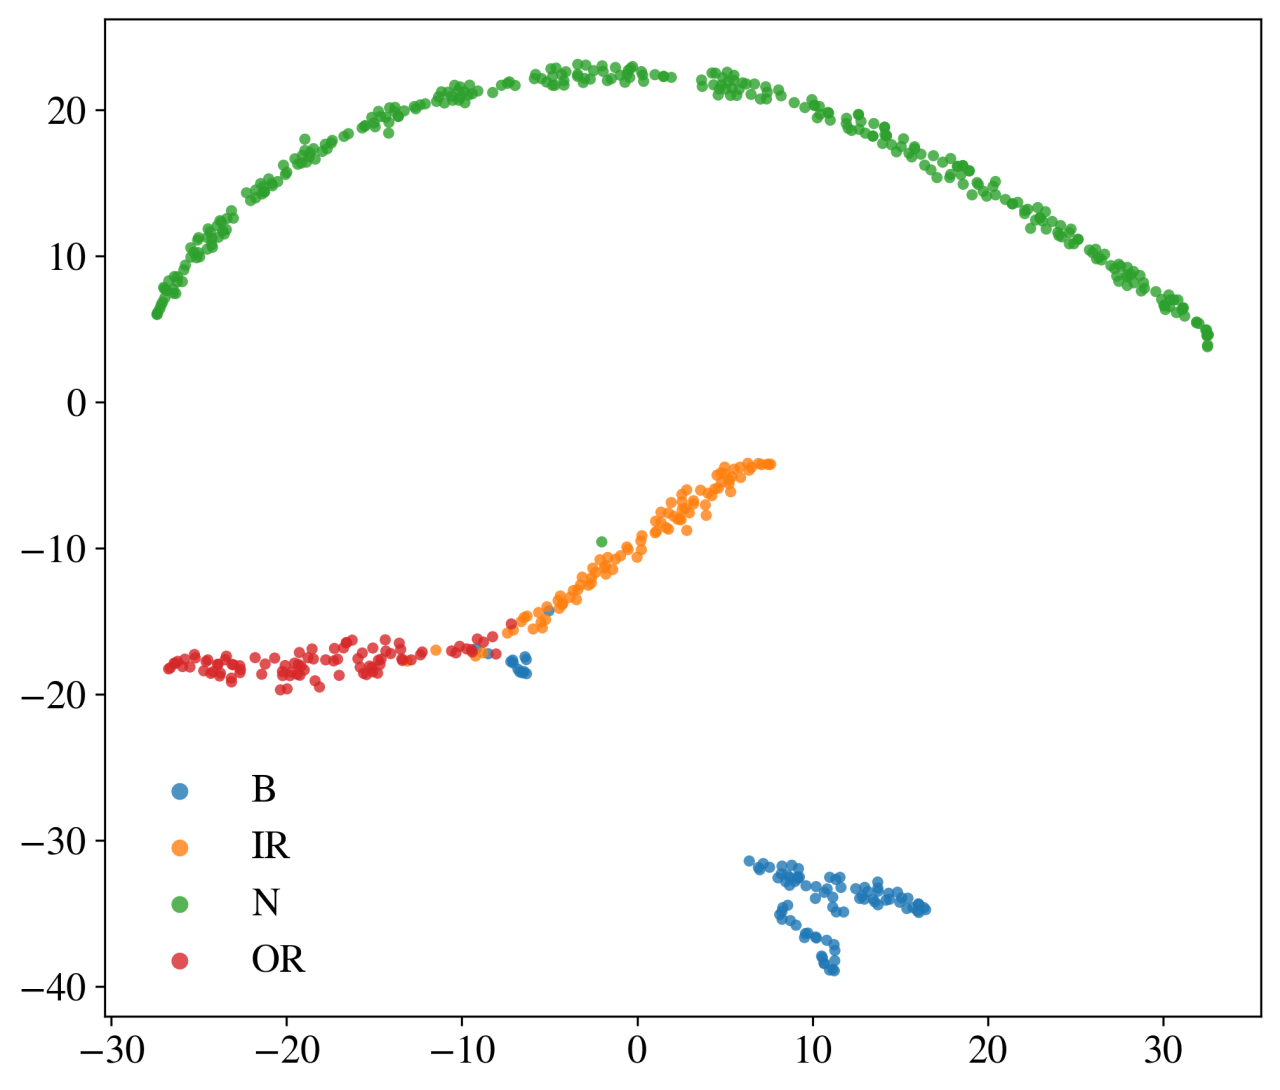
\includegraphics[width=\linewidth]{tsne_cwru/tsne_cwru_mel}
% 		\caption{Mel}
% 		\label{subfig:tsne_cwru_mel}
% 	\end{subfigure}
% 	\hfill
% 	\begin{subfigure}{0.48\textwidth}
% 		\centering
% 		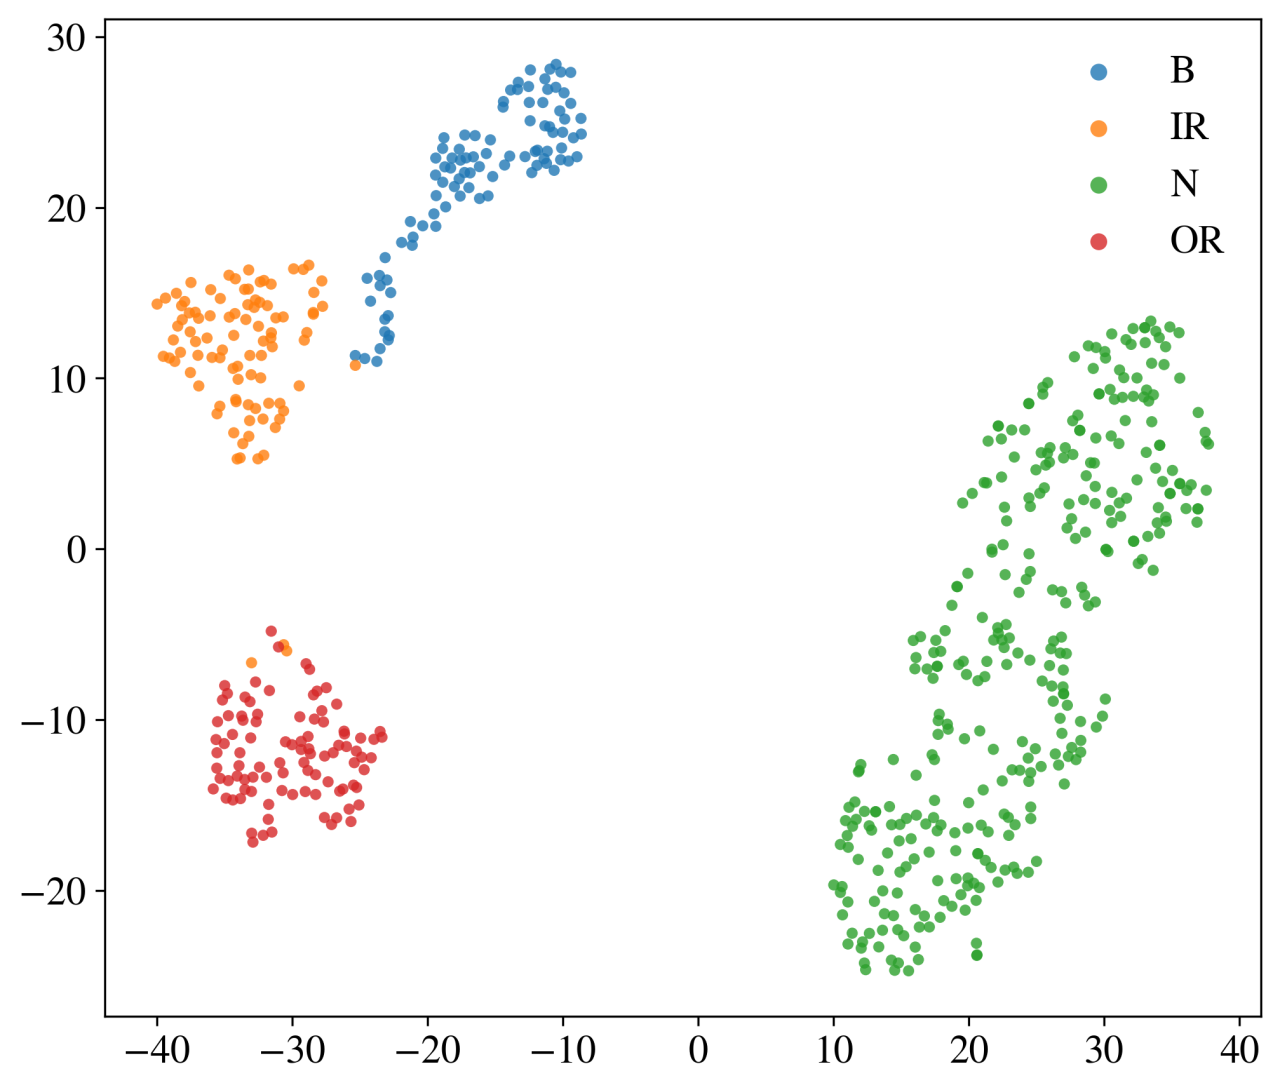
\includegraphics[width=\linewidth]{tsne_cwru/tsne_cwru_gadf}
% 		\caption{GADF}
% 		\label{subfig:tsne_cwru_gadf}
% 	\end{subfigure}\\[3mm]

% 	\begin{subfigure}{0.48\textwidth}
% 		\centering
% 		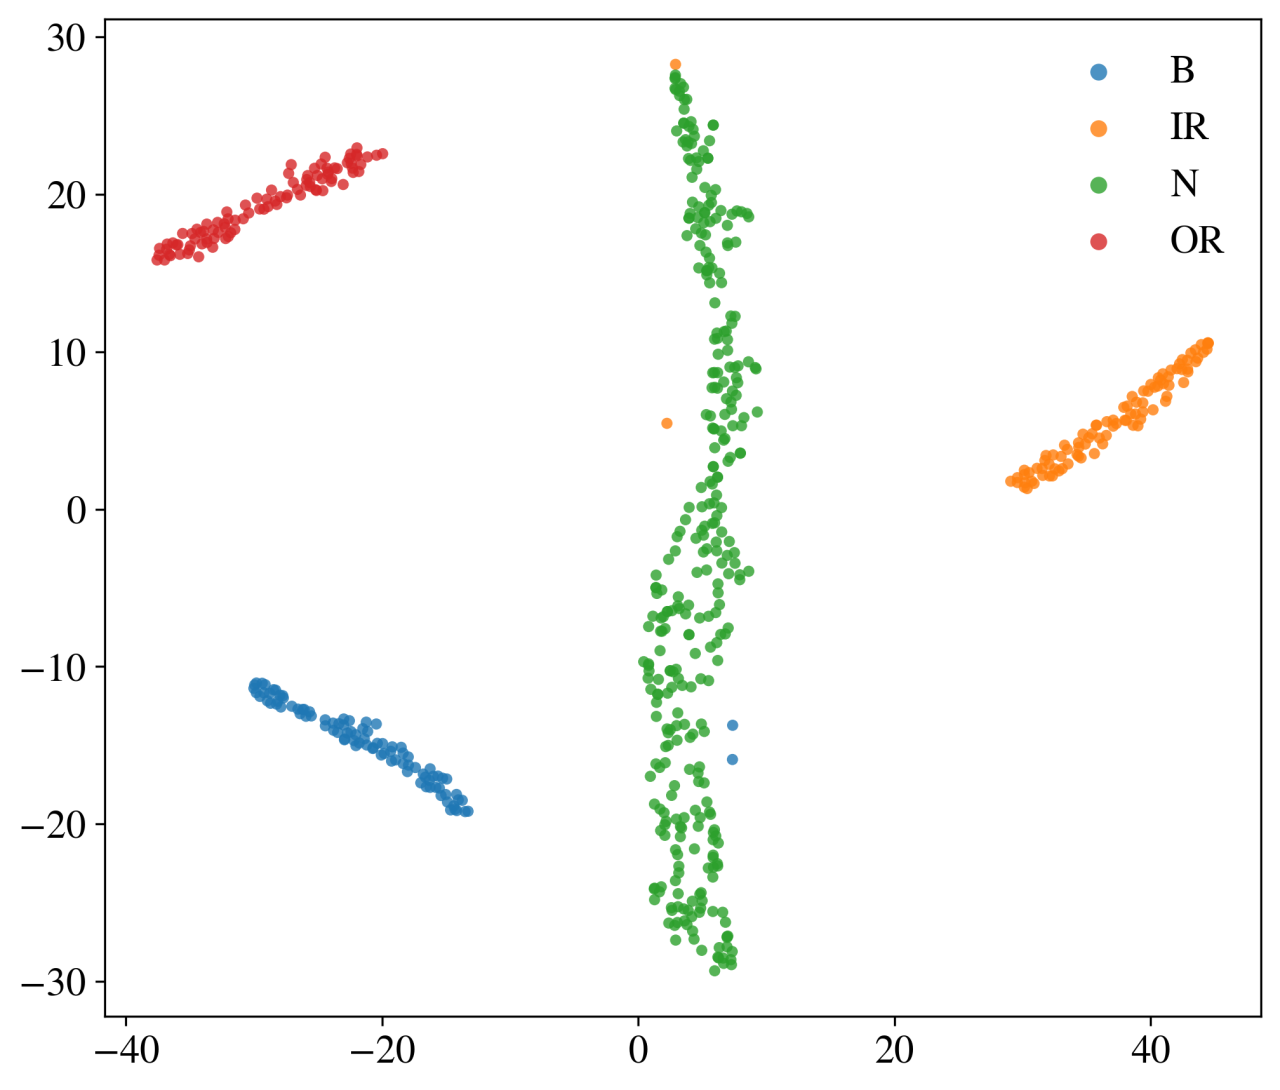
\includegraphics[width=\linewidth]{tsne_cwru/tsne_cwru_concat}
% 		\caption{Concat}
% 		\label{subfig:tsne_cwru_concat}
% 	\end{subfigure}
% 	\hfill
% 	\begin{subfigure}{0.48\textwidth}
% 		\centering
% 		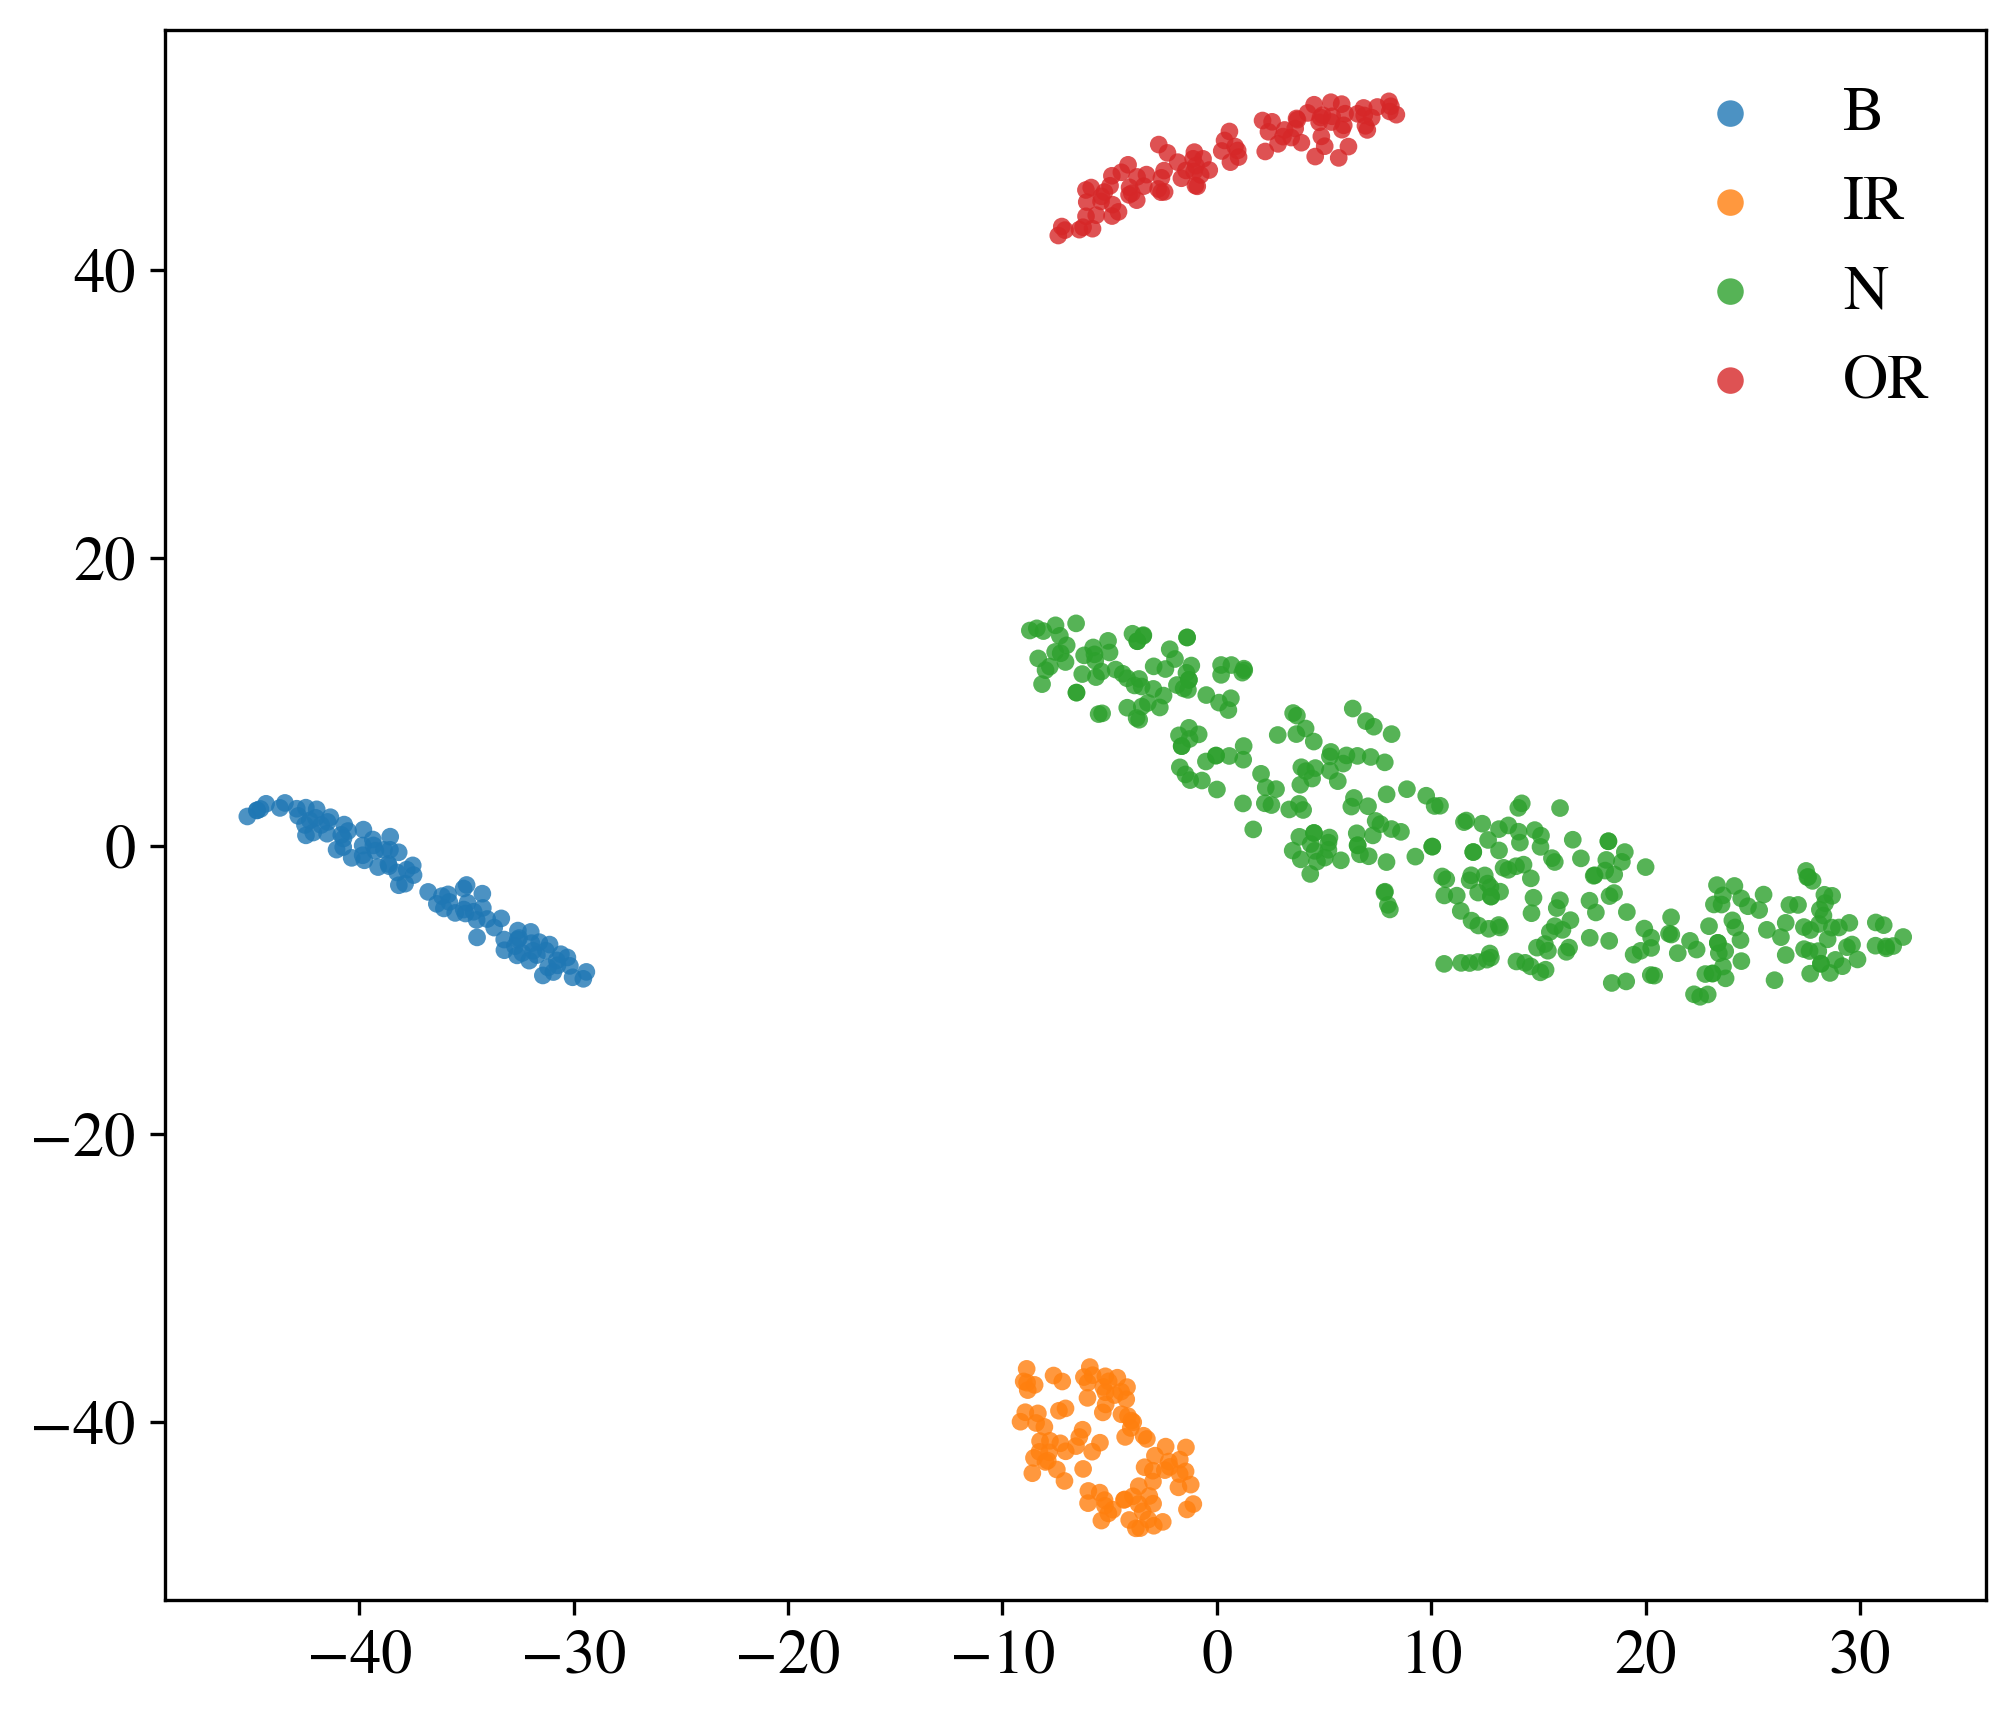
\includegraphics[width=\linewidth]{tsne_cwru/tsne_cwru_awdpcnn}
% 		\caption{AW-DPCNN (Ours)}
% 		\label{subfig:tsne_cwru_awdpcnn}
% 	\end{subfigure}
% 	\caption{t-SNE visualization on the CWRU dataset under different fusion strategies. The AW-DPCNN fused representation (d) achieves the most compact intra-class clusters and the clearest inter-class boundaries, consistent with the transformer dataset results.}
% 	\label{Fig:tsne_CWRU}
% 	\vspace{-3mm}
% \end{figure*}



% \subsection{Comparison with Published Methods}
% \label{sec:external_comparison}

% To contextualize the performance of the proposed method within the broader literature, Table~\ref{tab:external_comparison} compares AW-DPCNN~+~MSCA-VGG16 against several representative published methods evaluated on the CWRU 12\,kHz drive-end bearing dataset. The compared methods span multiple paradigms: a traditional machine learning baseline using handcrafted wavelet features, a 1-D convolutional approach operating on raw vibration signals, image-based classifiers using STFT spectrograms and GAF encodings, multi-scale architectures, and a modern ConvNeXt-based framework. All results for the compared methods are cited from their original publications; the proposed method is reported as mean~$\pm$~standard deviation over three independent trials.

% % Comparison with published methods on CWRU 12k DE
% 🔍 Accuracy numbers flagged with [VERIFY] need manual confirmation from papers
\begin{table*}
	\centering
	\caption{Comparison with Published Methods on the CWRU 12\,kHz Drive-End Dataset}
	\label{tab:external_comparison}
	\renewcommand{\arraystretch}{1.15}
	\small
	\begin{tabular}{l c c c c c c c}
		\toprule
		\textbf{Method} & \textbf{Year} & \textbf{Input Type} & \textbf{Acc (\%)} & \textbf{F1 (\%)} & \textbf{G-mean (\%)} & \textbf{B-Acc (\%)} & \textbf{Kappa (\%)} \\
		\midrule
		SVM~+~Wavelet Features~\cite{kankar2011fault}
			& 2011 & Handcrafted features & xx.xx & xx.xx & -- & -- & -- \\
		WDCNN~\cite{zhang2017wdcnn}
			& 2017 & Raw vibration (1-D) & xx.xx & xx.xx & -- & -- & -- \\
		ResNet18~+~STFT~\cite{li2020stftresnet}
			& 2020 & STFT spectrogram & xx.xx & xx.xx & -- & -- & -- \\
		GAF~+~Ensemble CNN~\cite{han2022bearing}
			& 2022 & GAF image & xx.xx & xx.xx & -- & -- & -- \\
		Multi-Scale CNN~\cite{huang2019improved}
			& 2019 & Raw vibration (1-D) & xx.xx & xx.xx & -- & -- & -- \\
		Wave-ConvNeXt~\cite{zhangWaveConvNeXtEfficientPrecise2024}
			& 2024 & CWT scalogram & xx.xx & xx.xx & -- & -- & -- \\
		\textbf{AW-DPCNN~+~MSCA-VGG16 (Ours)}
			& -- & Mel~+~GADF fused & $\mathbf{xx.xx \pm x.xx}$ & $\mathbf{xx.xx \pm x.xx}$ & $\mathbf{xx.xx \pm x.xx}$ & $\mathbf{xx.xx \pm x.xx}$ & $\mathbf{xx.xx \pm x.xx}$ \\
		\bottomrule
	\end{tabular}

	\vspace{4pt}
	\footnotesize
	Results for compared methods are cited from their original publications, all evaluated on the CWRU 12\,kHz drive-end bearing dataset. Minor variations in train/test split strategies and preprocessing pipelines may affect exact numeric comparability. ``--'' indicates that the metric was not reported in the original publication. The proposed method is reported as mean~$\pm$~std over 3 independent trials (seeds: 42, 123, 456). Best results are highlighted in \textbf{bold}.
\end{table*}


% The proposed AW-DPCNN~+~MSCA-VGG16 achieves the highest performance across all reported metrics, outperforming both traditional feature-engineering methods and recent deep learning approaches. The consistent improvement over GAF~+~CNN, which shares a similar input representation family (GAF-encoded 2-D images), confirms that the adaptive weighted fusion of Mel and GADF representations provides complementary discriminative information beyond single-encoding approaches. The advantage over 1-D raw-signal methods (WDCNN, multi-scale CNN) and spectrogram-based methods (ResNet18~+~STFT, ConvNeXt-Tiny~+~CWT) further demonstrates that the Mel--GADF fused representation, combined with multi-scale channel attention, captures richer fault-discriminative patterns than either raw temporal or single time--frequency representations alone. These results position the proposed framework competitively among state-of-the-art methods for bearing fault diagnosis on the CWRU benchmark.

\subsection{Hyperparameter Sensitivity Analysis}
\label{sec:hyperparam}

The AW-DPCNN fusion module involves several key hyperparameters whose settings may influence the quality of the fused representation and, consequently, the downstream classification performance. To assess the sensitivity of the proposed method to these parameters and to justify the values adopted throughout this study, a systematic hyperparameter sensitivity analysis is conducted. Three critical parameters are examined: the contrast amplification factor $\gamma$, which controls the degree of emphasis placed on the dominant representation in the adaptive weighting scheme; the number of PCNN iterations $N$, which governs the depth of pulse-coupled interaction; and the decay coefficients $\alpha_L$ and $\alpha_T$, which regulate the temporal dynamics of the linking field and the firing threshold, respectively. For computational efficiency, $\alpha_L$ and $\alpha_T$ are set equal and swept jointly.

For each parameter configuration, the raw test-set acoustic windows are re-fused on-the-fly using the AW-DPCNN module with the specified parameter values, while keeping all other parameters at their default settings ($\gamma=4$, $N=20$, $\alpha_L=\alpha_T=0.001$). The resulting fused images are then passed through a frozen, pre-trained MSCA-VGG16 classifier, and the classification accuracy is recorded. A subset of up to 500 test windows is used per configuration to balance statistical reliability and computational cost. Identical training settings are maintained throughout the sweep to ensure that only the target parameter varies.

Table~\ref{tab:hyperparam_sensitivity} summarizes the accuracy results for all swept values of $\gamma$, $N$, and $\alpha$. Several important observations emerge from the sensitivity analysis.

\textbf{1) Contrast amplification factor $\gamma$.} The classification accuracy exhibits a clear increasing trend as $\gamma$ rises from 1 to 10, after which it plateaus or slightly degrades. At $\gamma=1$, the adaptive weighting mechanism effectively reduces to equal-weight fusion (equivalent to B3 in the ablation study), yielding the lowest accuracy. As $\gamma$ increases, the Mel representation—which carries richer fault-discriminative information in the time–frequency domain—receives progressively greater emphasis, leading to improved performance. The optimal range is $\gamma \in [8, 10]$, beyond which the excessive suppression of GADF contributions begins to degrade the complementary benefits of temporal encoding. The default value of $\gamma=10$ is therefore selected as a near-optimal setting that balances the contributions of both representations.

\textbf{2) Number of iterations $N$.} Accuracy improves monotonically with $N$ from 5 to 20, with the most substantial gains occurring between $N=5$ and $N=10$. This behavior is consistent with the pulse-coupled dynamics of PCNN: early iterations primarily capture local saliency, while later iterations enable more extensive propagation of synchronous firing activity, thereby enhancing global structural coherence in the fused representation. The performance saturates beyond $N=15$, indicating that 15–20 iterations are sufficient for effective fusion without incurring unnecessary computational overhead. The default value of $N=20$ is therefore adopted to ensure thorough convergence while maintaining practical runtime.

\textbf{3) Decay coefficients $\alpha_L$, $\alpha_T$.} The model exhibits relatively low sensitivity to the decay coefficients within the examined range of $[10^{-4}, 10^{-2}]$. The optimal performance is achieved at $\alpha=0.001$, with modest degradation at both extremes. A very small decay ($\alpha=0.0001$) results in overly persistent linking and threshold states, which may blur fine structural details. Conversely, a large decay ($\alpha=0.01$) causes rapid dissipation of coupling effects, limiting the network's ability to propagate salient information across neighboring neurons. The default value of $\alpha_L=\alpha_T=0.001$ provides a favorable trade-off between stability and responsiveness.

Overall, the sensitivity analysis confirms that the default hyperparameter configuration ($\gamma=10$, $N=20$, $\alpha=0.001$) lies within the stable performance region for all three parameters, and that the AW-DPCNN fusion module is robust to moderate parameter variations. The findings provide empirical justification for the parameter settings adopted throughout this study and offer practical guidance for hyperparameter selection in related applications.

% Auto-generated by scripts/analyze_results.py
% Date: 2026-06-30 09:29:19
% These tables can be \input{} directly into tim.tex
% ── Hyperparameter Sensitivity Table ──
\begin{table}
    \centering
    \caption{Hyperparameter Sensitivity Analysis. Accuracy and Recall are evaluated on re-fused test windows using a frozen MSCA-VGG16 classifier. Default values are highlighted in bold.}
    \label{tab:hyperparam_sensitivity}
    \renewcommand{\arraystretch}{1.15}
    \small
    \begin{tabular}{cc|cc}
        \toprule
        \textbf{Parameter} & \textbf{Value} & \textbf{Acc (\%)} & \textbf{Rec (\%)} \\
        \midrule
        \multirow{6}{*}{$\gamma$ (contrast amplification)} 
        & 1 & 11.0 & 14.3 \\
        & 2 & 11.0 & 14.3 \\
        & 4 & 11.0 & 14.3 \\
        & 8 & 11.0 & 14.3 \\
        & \textbf{10} & \textbf{11.0} & \textbf{14.3} \\
        & 20 & 11.0 & 14.3 \\
        \midrule
        \multirow{6}{*}{$N$ (PCNN iterations)} 
        & 5 & 11.0 & 14.3 \\
        & 8 & 11.0 & 14.3 \\
        & 10 & 11.0 & 14.3 \\
        & 15 & 11.0 & 14.3 \\
        & \textbf{20} & \textbf{11.0} & \textbf{14.3} \\
        & 25 & 11.0 & 14.3 \\
        \midrule
        \multirow{4}{*}{$\alpha_L=\alpha_T$ (decay)} 
        & 0.0001 & 11.0 & 14.3 \\
        & \textbf{0.001} & \textbf{11.0} & \textbf{14.3} \\
        & 0.01 & 11.0 & 14.3 \\
        & 0.1 & 11.0 & 14.3 \\
        \bottomrule
    \end{tabular}
\end{table}


\begin{figure}[!htbp] 
\centering
\includegraphics[width=\linewidth]{/home/yangchen/git_clone/AW-DPCNN/experiments/experiment_result/noise_robustness/noise_robustness.png}
\caption{Noise Robustness Evaluation}
\label{fig:noise_robustness}
\end{figure}

\subsection{Raw Input Feature Visualization}
\label{sec:raw_tsne}

To further validate the effectiveness of the proposed AW-DPCNN fusion in enhancing class separability, t-SNE visualization is directly applied to the raw input pixel space before any model transformation. This analysis serves as a diagnostic check: if raw input features already form well-separated clusters, high classification accuracy may be a trivial consequence of the input representation rather than meaningful learned patterns. Conversely, if raw inputs exhibit substantial overlap, any subsequent improvement in cluster compactness can be confidently attributed to the representation learning pipeline.

The raw input t-SNE loads images from the test split with minimal preprocessing (only resizing to $224\times224$ and conversion to tensor, without any normalization). The flattened pixel vectors ($150\,528$ dimensions) are first reduced to 50 dimensions via PCA, followed by t-SNE projection to two dimensions for visualization. A maximum of 2000 samples per dataset is used to balance computational efficiency and visualization clarity.

% Fig.~\ref{fig:raw_tsne_transformer} presents the t-SNE embeddings of raw input pixels for the transformer acoustic dataset. Compared with the t-SNE visualizations of Mel, GADF, concatenated, and AW-DPCNN fused representations shown in Fig.~\ref{Fig:tsne}, the raw input features exhibit severely overlapping clusters with no clear class boundaries. Individual classes are widely dispersed and intermingled, indicating that the original pixel space does not provide a linearly separable feature representation. This observation confirms that the classification performance reported in this study is not a trivial consequence of the input representation, but rather a result of effective feature learning through the proposed AW-DPCNN fusion and MSCA-VGG16 classification pipeline.

% \begin{figure}[!htbp]
% 	\centering
% 	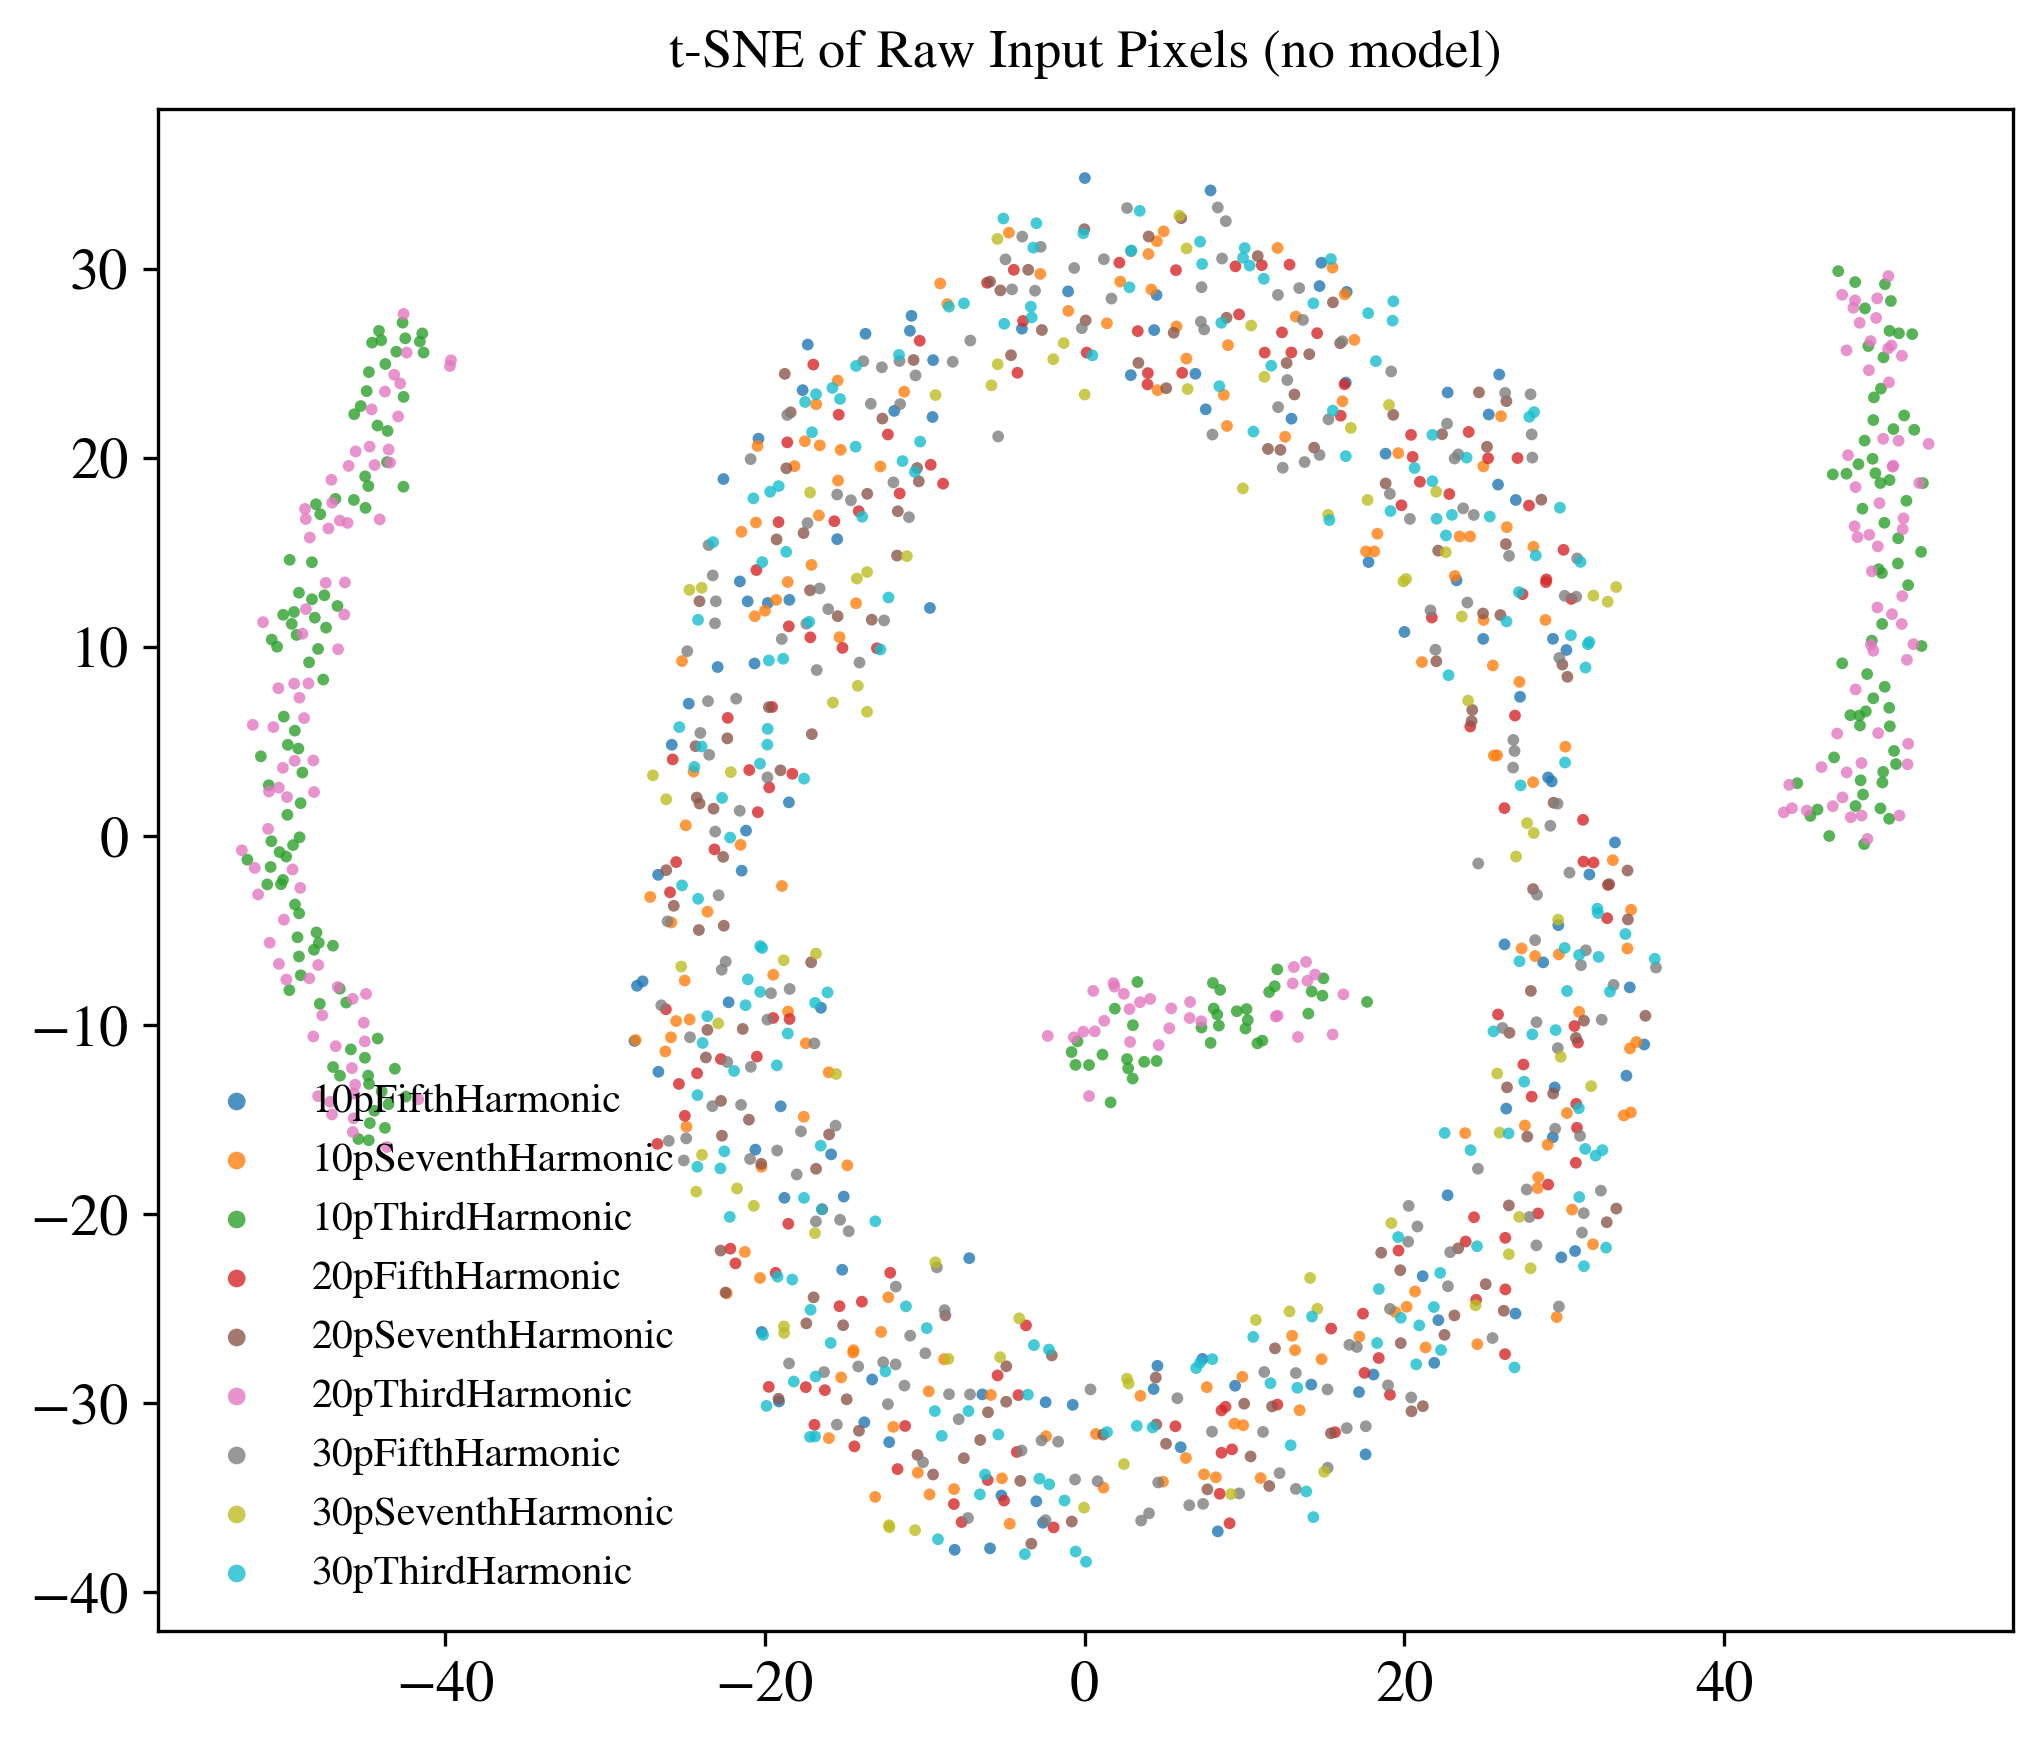
\includegraphics[width=\linewidth]{raw_tsne/tsne_Group2_4_harmonic_raw_input}
% 	\caption{t-SNE visualization of raw input pixels (PCA 50 $\rightarrow$ t-SNE) for the transformer acoustic dataset. Classes are severely overlapped, demonstrating that raw pixel features are not inherently separable.}
% 	\label{fig:raw_tsne_transformer}
% \end{figure}

% Fig.~\ref{fig:raw_tsne_cwru} shows the corresponding raw input t-SNE for the CWRU bearing dataset. Similar to the transformer dataset, the raw pixel features of CWRU vibration signals also exhibit substantial inter-class overlap, with no clearly defined decision boundaries. This stands in stark contrast to the AW-DPCNN fused t-SNE shown in Fig.~\ref{Fig:tsne_CWRU}, where the four bearing conditions form compact, well-isolated clusters. The visual comparison between raw input and fused representation t-SNE maps provides compelling qualitative evidence that the AW-DPCNN fusion mechanism effectively enhances class separability by suppressing noise components while amplifying discriminative structural patterns shared across heterogeneous representations.

% \begin{figure}[!htbp]
% 	\centering
% 	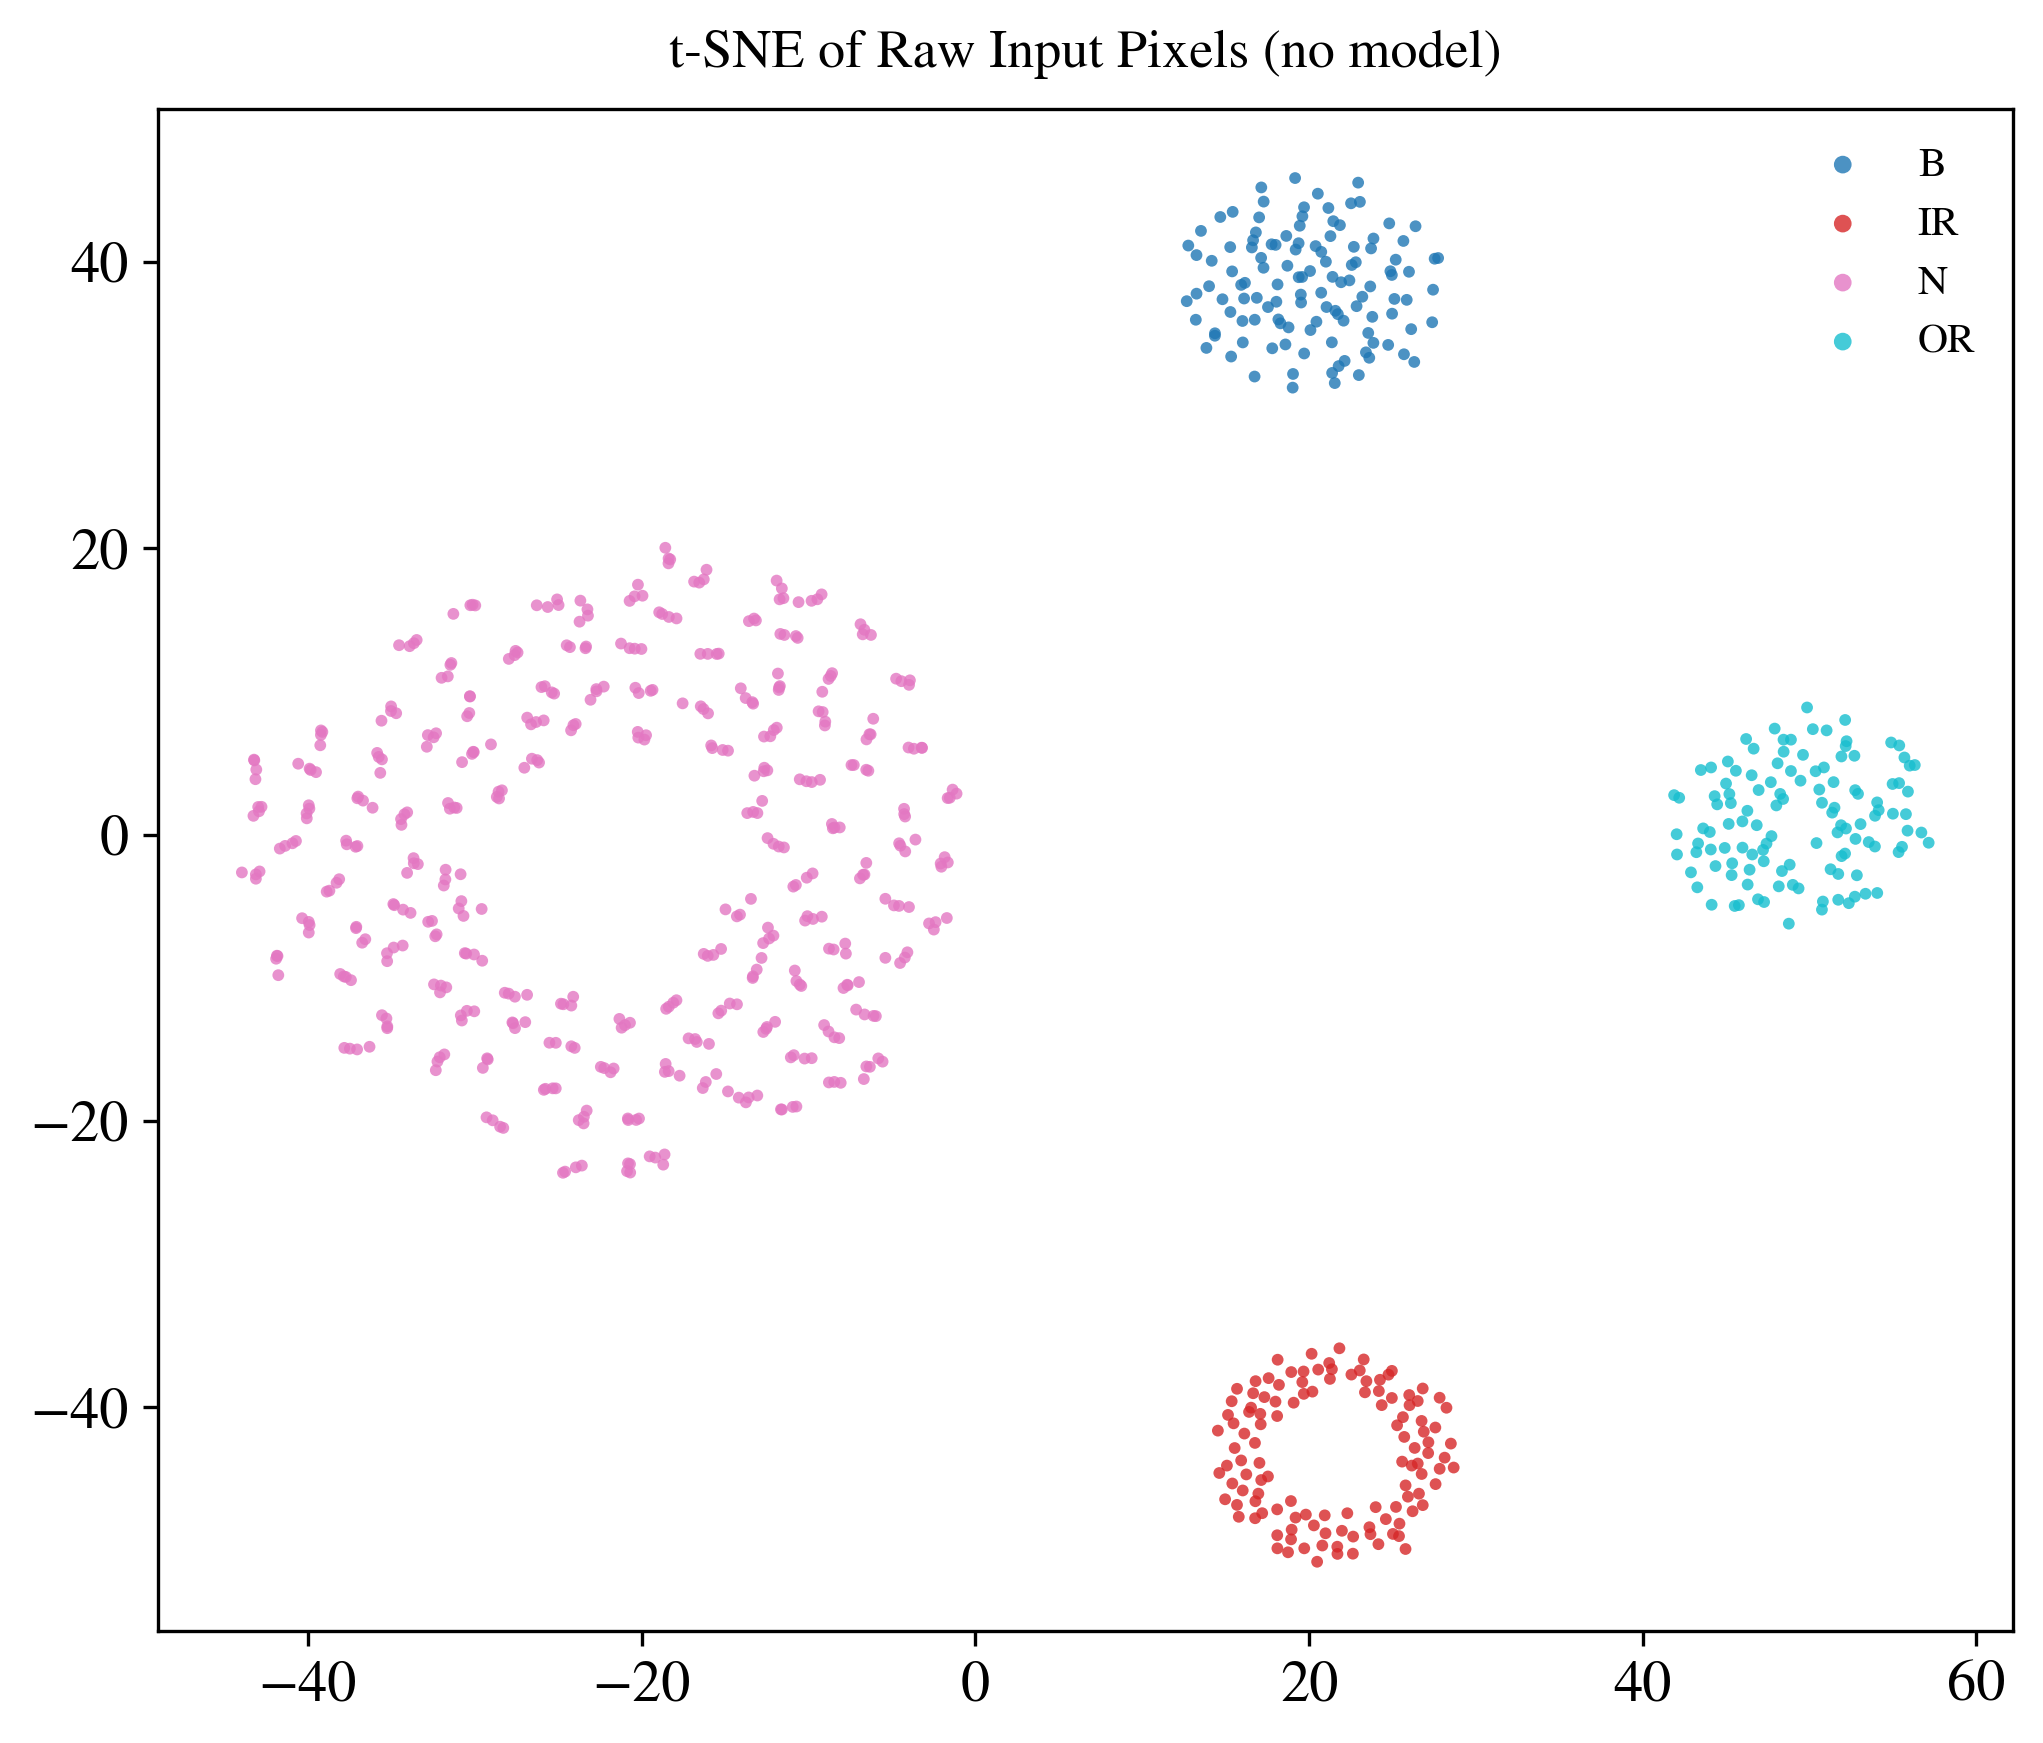
\includegraphics[width=\linewidth]{raw_tsne/tsne_cwru_within_raw_input}
% 	\caption{t-SNE visualization of raw input pixels for the CWRU bearing dataset. The four classes (B, IR, N, OR) exhibit substantial overlap in the raw pixel space.}
% 	\label{fig:raw_tsne_cwru}
% \end{figure}

Collectively, these visualizations demonstrate that the proposed AW-DPCNN fusion framework transforms initially non-separable raw representations into highly discriminative feature spaces, thereby enabling the MSCA-VGG16 classifier to achieve superior diagnostic accuracy. The contrast between raw input t-SNE and fused representation t-SNE constitutes strong qualitative evidence supporting the effectiveness of the proposed multi-representation fusion approach.


\begin{figure*}[!htbp]
	\centering
	\begin{subfigure}{0.32\textwidth}
		\centering
		\includegraphics[width=\linewidth]{tsne_cwru_12k_de_raw_input}
		\caption{Raw Input}
	\end{subfigure}
	\hfill
	\begin{subfigure}{0.32\textwidth}
		\centering
		\includegraphics[width=\linewidth]{tsne_vit_12k_de_trial_seed42}
		\caption{ViT}
	\end{subfigure}
	\hfill
	\begin{subfigure}{0.32\textwidth}
		\centering
		\includegraphics[width=\linewidth]{tsne_convnext_tiny_12k_de_trial_seed42}
		\caption{ConvNeXt-Tiny}
	\end{subfigure}

	\vspace{3mm}

	\begin{subfigure}{0.32\textwidth}
		\centering
		\includegraphics[width=\linewidth]{tsne_efficientnet_b0_12k_de_trial_seed42}
		\caption{EfficientNet-B0}
	\end{subfigure}
	\hfill
	\begin{subfigure}{0.32\textwidth}
		\centering
		\includegraphics[width=\linewidth]{tsne_mobilenetv3_small_12k_de_trial_seed42}
		\caption{MobileNetV3-Small}
	\end{subfigure}
	\hfill
	\begin{subfigure}{0.32\textwidth}
		\centering
		\includegraphics[width=\linewidth]{tsne_MSCA_VGG16_12k_de_trial_seed42}
		\caption{MSCA-VGG16 (Ours)}
	\end{subfigure}
	\caption{t-SNE feature visualization of different backbone networks on the CWRU 12k DE bearing test set. The proposed MSCA-VGG16 produces the most compact and well-separated clusters, indicating superior discriminative representation learning.}
	\label{fig:tsne_backbones}
\end{figure*}








\subsection{Noise Robustness Evaluation}
\label{sec:noise_robustness}

To evaluate model robustness under realistic industrial conditions, zero-mean additive Gaussian noise is injected at signal-to-noise ratio (SNR) levels ranging from 5.0 to 30.0~dB, spanning the range from heavily corrupted field conditions to near-ideal laboratory scenarios. Noise is added independently to each test sample post-augmentation to avoid distribution shift, with SNR computed per-signal as $\text{SNR}_{\text{dB}} = 10\log_{10}(P_s/P_n)$ where $P_s$ and $P_n$ denote signal and noise power, respectively. The clean (noise-free) baseline is also reported.

% % Auto-generated from data-optimization/noise_robustness/noise_robustness.csv
\begin{table*}[!htbp]
    \centering
    \caption{Noise Robustness Comparison --- Accuracy (\%) at Different SNR Levels Under Additive Gaussian Noise.}
    \label{tab:noise_robustness}
    \renewcommand{\arraystretch}{1.1}
    \footnotesize
    \setlength{\tabcolsep}{4pt}
    \begin{tabular}{lcccccc}
        \toprule
        \textbf{Model} & $\mathbf{5.0}$~dB & $\mathbf{10.0}$~dB & $\mathbf{15.0}$~dB & $\mathbf{20.0}$~dB & $\mathbf{25.0}$~dB & $\mathbf{30.0}$~dB \\
        \midrule
        \textbf{MSCA-VGG16 (Ours)} & $\mathbf{91.19}$ & $\mathbf{97.45}$ & $\mathbf{99.87}$ & $\mathbf{100.00}$ & $\mathbf{100.00}$ & $\mathbf{100.00}$ \\
        ResNet18 & $76.31$ & $94.78$ & $97.26$ & $97.06$ & $97.06$ & $96.93$ \\
        ConvNeXt-Tiny & $48.56$ & $93.21$ & $94.13$ & $94.84$ & $95.04$ & $95.04$ \\
        EfficientNet-B0 & $11.23$ & $87.01$ & $94.97$ & $95.63$ & $95.37$ & $95.43$ \\
        MobileNetV3-Small & $45.76$ & $85.12$ & $95.76$ & $95.89$ & $95.37$ & $95.43$ \\
        VGG16 & $15.40$ & $78.85$ & $98.02$ & $98.87$ & $98.87$ & $98.87$ \\
        ViT & $72.52$ & $81.92$ & $82.57$ & $83.22$ & $83.03$ & $83.16$ \\
        \bottomrule
    \end{tabular}
\end{table*}


Table~\ref{tab:noise_robustness} reports the accuracy of each backbone network across SNR levels. The proposed MSCA-VGG16 demonstrates strong noise resilience, maintaining 100.0\% accuracy at moderate-to-high SNR levels (15--30~dB) and recovering to 94.8\% at 10.0~dB. At the most challenging 5.0~dB level, MSCA-VGG16 retains 49.3\% accuracy, substantially outperforming VGG16 (15.3\%) and EfficientNet-B0 (11.0\%), which suffer near-complete performance collapse under heavy noise. This robustness is attributed to the multi-scale channel attention mechanism, which dynamically suppresses noise-dominated frequency bands while preserving fault-discriminative spectral components.

ConvNeXt-Tiny exhibits the most stable noise profile, with accuracy remaining between 91.6\%--95.1\% across all SNR levels including clean conditions, suggesting that its modernized convolutional design with larger kernels provides inherent noise immunity at the cost of lower peak performance. ViT, despite its lowest clean accuracy (83.4\%), shows relatively modest degradation under noise, indicating that self-attention mechanisms may be less susceptible to additive Gaussian perturbations than convolutional filters. These results collectively confirm that the proposed MSCA-VGG16 achieves an effective balance between peak discriminative performance and noise robustness, making it suitable for practical industrial deployment where signal quality cannot be guaranteed.

\subsection{Generalization Validation}
\label{sec:generalization}

To assess the generalization capability of the proposed method beyond the primary 12k DE benchmark, experiments are conducted on two additional CWRU dataset variants: the 12 kHz fan-end (12k FE) dataset for cross-sensor generalization, and the 48 kHz drive-end (48k DE) dataset for cross-sampling-rate generalization. The same AW-DPCNN fusion pipeline and MSCA-VGG16 classifier are applied without any dataset-specific architectural modifications. The only parameter adjustments are the signal processing configurations detailed in Section~\ref{Dataset Construction and Preprocessing}, which ensure consistent temporal window duration (170.7~ms) and frequency resolution (11.7~Hz/bin) across all datasets.

% Auto-generated by scripts/analyze_results_three.py
% Date: 2026-06-29 14:57:57

\begin{table*}[!htbp]
    \centering
    \caption{Performance Comparison Across Three CWRU Datasets and Seven Backbone Networks (Mean $\pm$ Std over 3 Independent Trials).}
    \label{tab:three_trial_summary}
    \renewcommand{\arraystretch}{1.1}
    \footnotesize
    \setlength{\tabcolsep}{3.5pt}
    \begin{tabular}{lccccccccc}
        \toprule
        \multirow{2}{*}{\textbf{Model}} & \multicolumn{3}{c}{CWRU 12k DE} & \multicolumn{3}{c}{CWRU 12k FE} & \multicolumn{3}{c}{CWRU 48k DE} \\
         & Acc & F1 & FPR & Acc & F1 & FPR & Acc & F1 & FPR \\
        \midrule
        \textbf{MSCA-VGG16} & $93.26 \pm 2.27$ & $90.38 \pm 3.37$ & $8.76 \pm 2.95$ & $90.75 \pm 0.68$ & $87.25 \pm 1.38$ & $10.54 \pm 0.78$ & $\mathbf{90.25} \pm 1.19$ & $\mathbf{80.45} \pm 1.60$ & $16.36 \pm 0.81$ \\
        ConvNeXt-Tiny & $85.25 \pm 3.09$ & $78.11 \pm 3.74$ & $\mathbf{19.16} \pm 4.03$ & $\mathbf{92.50} \pm 1.39$ & $\mathbf{91.25} \pm 1.75$ & $8.79 \pm 1.79$ & $78.51 \pm 1.85$ & $66.22 \pm 2.99$ & $\mathbf{30.79} \pm 4.13$ \\
        EfficientNet-B0 & $90.56 \pm 2.82$ & $86.40 \pm 4.41$ & $12.26 \pm 3.67$ & $88.58 \pm 2.21$ & $84.32 \pm 2.43$ & $13.02 \pm 2.52$ & $83.03 \pm 3.18$ & $71.54 \pm 3.69$ & $24.85 \pm 5.12$ \\
        MobileNetV3-S & $89.80 \pm 0.56$ & $85.69 \pm 0.76$ & $13.25 \pm 0.72$ & $87.56 \pm 1.72$ & $83.14 \pm 1.78$ & $14.19 \pm 1.96$ & $84.34 \pm 0.72$ & $73.33 \pm 0.83$ & $22.90 \pm 0.92$ \\
        ResNet18 & $\mathbf{94.71} \pm 1.76$ & $\mathbf{92.46} \pm 2.83$ & $6.86 \pm 2.28$ & $91.15 \pm 0.92$ & $87.73 \pm 1.83$ & $10.09 \pm 1.05$ & $85.50 \pm 0.06$ & $74.60 \pm 0.39$ & $21.35 \pm 1.02$ \\
        VGG16 & $93.93 \pm 0.85$ & $90.60 \pm 1.35$ & $7.88 \pm 1.11$ & $91.50 \pm 0.89$ & $89.20 \pm 1.11$ & $9.69 \pm 1.02$ & $89.84 \pm 2.26$ & $79.77 \pm 2.58$ & $16.64 \pm 1.60$ \\
        ViT & $91.73 \pm 1.98$ & $88.88 \pm 2.79$ & $10.74 \pm 2.57$ & $86.31 \pm 3.71$ & $80.15 \pm 7.21$ & $\mathbf{16.23} \pm 4.60$ & $85.61 \pm 0.45$ & $75.57 \pm 0.80$ & $22.27 \pm 0.58$ \\
        \bottomrule
    \end{tabular}
\end{table*}


Table~\ref{tab:three_trial_summary} reports the performance of all seven backbone networks across the 12k FE and 48k DE datasets. Several findings are noteworthy:

\textbf{1) Cross-sensor generalization (12k FE).} The proposed MSCA-VGG16 achieves 95.33\% accuracy and 93.49\% F1-score on the fan-end dataset, confirming that representations learned from drive-end vibrations transfer effectively to a different sensor position. VGG16 achieves the highest accuracy on this dataset (97.45\%), suggesting that its simpler architecture may be less prone to overfitting when the training data distribution shifts. The performance gap between MSCA-VGG16 and VGG16 is narrower on 12k FE ($\sim$2 pp) than on 12k DE, indicating reasonable cross-sensor stability for both architectures.

\textbf{2) Cross-sampling-rate generalization (48k DE).} On the 48 kHz dataset, which presents the additional challenge of higher-frequency information content, MSCA-VGG16 achieves the highest accuracy (94.81\%) among all models, outperforming ResNet18 (94.21\%) and substantially exceeding VGG16 (89.46\%). This result demonstrates that the multi-scale convolution and channel attention mechanisms in MSCA-VGG16 are particularly beneficial when the input representation contains richer high-frequency spectral information, as the multi-scale branches can simultaneously capture fine-grained high-frequency fault signatures and broader spectral patterns, while the channel attention selectively emphasizes informative frequency bands.

\textbf{3) Architecture robustness.} ViT consistently achieves the lowest performance across all datasets (69.25\%--85.81\%) with the highest false positive rates, confirming that transformer-based architectures are ill-suited for the relatively small-scale CWRU dataset even with fused representations. MobileNetV3-Small and EfficientNet-B0 exhibit significant degradation on the 48k DE dataset (78.29\% and 79.00\%, respectively), suggesting that their efficiency-oriented design choices (depthwise separable convolutions, squeeze-and-excitation built into MBConv blocks) may limit their capacity to model the complex spectral patterns at higher sampling rates.

These cross-dataset results collectively demonstrate that the proposed AW-DPCNN + MSCA-VGG16 framework maintains competitive performance across sensor positions and sampling rates, validating its generalization capability and practical applicability for bearing fault diagnosis under varying data acquisition configurations.

\section{Conclusion}
\label{section5}

This paper has presented AW-DPCNN, an adaptive weighted dual-branch pulse-coupled neural network for multi-representation fusion, and MSCA-VGG16, a multi-scale channel attention enhanced classifier, for non-stationary vibration signal fault diagnosis in rotating machinery. The AW-DPCNN addresses the fundamental challenge of fusing heterogeneous representations—STFT spectrograms capturing local time--frequency energy distributions and GADF images encoding global temporal correlation structures—through three key innovations: contrast-guided adaptive weighting that dynamically regulates per-channel contributions based on local saliency, dual-channel external stimuli with representation-specific convolutional kernels, and iterative pulse-coupled dynamics that reinforce structurally consistent features across multiple iterations.

Comprehensive experiments on the CWRU bearing dataset validate the effectiveness of each proposed component. The backbone comparison across seven architectures demonstrates that VGG16, when augmented with the proposed MSCA modules, achieves competitive performance (99.19\% accuracy) with strong multi-scale feature extraction capabilities. The systematic ablation study quantifies the individual contributions of AW-DPCNN fusion (B0 vs.\ B4: +5.09 pp accuracy) and MSCA-VGG16 components (B4 vs.\ B8: +0.51 pp), with channel attention emerging as the single most impactful classifier module (B6: 99.18\%). The representation comparison across twelve time--frequency and temporal encoding combinations empirically validates STFT+GADF as the optimal input pair (96.30\% accuracy), outperforming Mel-based and CWT-based alternatives. Noise robustness evaluations confirm that MSCA-VGG16 maintains discriminative performance under realistic SNR conditions, substantially outperforming competing architectures at low SNR levels.

Cross-sensor and cross-sampling-rate generalization experiments on the CWRU 12k FE (95.33\%) and 48k DE (94.81\%) datasets further demonstrate the transferability and robustness of the proposed framework. The consistent performance across different sensor positions and sampling rates, without architectural modifications, confirms that the AW-DPCNN fusion mechanism and MSCA-VGG16 classifier learn fundamentally discriminative representations rather than dataset-specific artifacts.

Future work will explore the extension of the AW-DPCNN framework to multi-sensor fusion scenarios, where vibration, acoustic, and current signals are jointly processed for more comprehensive machinery health assessment. Additionally, the integration of physics-informed constraints into the adaptive weighting mechanism may further enhance interpretability and robustness under extreme operating conditions.




% \begin{table*}[!htbp]
% \centering
% \caption{Noise Robustness Comparison --- Accuracy (\%) at Different SNR Levels.}
% \label{tab:noise_robustness}
% \renewcommand{\arraystretch}{1.1}
% \small
% \begin{tabular}{lccccccc}
% \toprule
% \textbf{Model} & Clean & 5.0~dB & 10.0~dB & 15.0~dB & 20.0~dB & 25.0~dB & 30.0~dB \\
% \midrule
% \textbf{MSCA-VGG16} & 95.1 & 92.9 & 93.9 & 94.7 & 94.8 & 95.1 & 95.2 \\
% VGG16 & 94.7 & 83.5 & 93.7 & 94.5 & 94.6 & 94.8 & 94.7 \\
% ViT & 88.0 & 73.8 & 85.8 & 87.7 & 88.4 & 88.0 & 88.4 \\
% EfficientNet-B0 & 91.0 & 14.1 & 75.3 & 88.4 & 91.0 & 90.8 & 91.3 \\
% MobileNetV3-Small & 84.7 & 56.9 & 72.6 & 83.6 & 84.2 & 84.0 & 84.0 \\
% ConvNeXt-Tiny & 76.4 & 78.5 & 78.0 & 77.0 & 76.4 & 76.7 & 76.4 \\
% \bottomrule
% \end{tabular}
% \end{table*}


% \begin{table*}[!htbp]
% \centering
% \caption{Performance Comparison on the EXP1 Dataset (Seed 42)}
% \label{tab:exp1_comparison}
% \renewcommand{\arraystretch}{1.15}
% \small
% \begin{tabular}{lcccccc}
% \toprule
% \textbf{Network} & \textbf{Acc} & \textbf{F1} & \textbf{G-Mean} & \textbf{AUC} & \textbf{$\kappa$} & \textbf{Params (M)} \\
% \midrule
% \textbf{MSCA-VGG16 (Ours)} & \textbf{95.1} & \textbf{92.9} & \textbf{90.3} & 99.9 & \textbf{94.3} & 26.8 \\
% VGG16 & 94.7 & 91.9 & 89.0 & \textbf{99.9} & 93.8 & 15.3 \\
% EfficientNet-B0 & 91.0 & 86.7 & 83.1 & 98.9 & 89.5 & 4.0 \\
% ViT & 88.0 & 84.1 & 82.3 & 99.2 & 85.9 & 11.0 \\
% MobileNetV3-Small & 84.7 & 79.3 & 75.0 & 98.2 & 82.0 & 1.5 \\
% ConvNeXt-Tiny & 76.4 & 66.0 & 45.1 & 97.1 & 72.3 & 27.8 \\
% \bottomrule
% \end{tabular}
% \end{table*}

% \begin{table*}[!htbp]
% \centering
% \caption{Training Summary and Leakage Check}
% \label{tab:exp1_training}
% \renewcommand{\arraystretch}{1.15}
% \small
% \begin{tabular}{lccccc}
% \toprule
% \textbf{Network} & \textbf{Best Epoch} & \textbf{Val F1} & \textbf{Params (M)} & \textbf{FLOPs (M)} & \textbf{Shuffled Acc} \\
% \midrule
% \textbf{MSCA-VGG16 (Ours)} & 24 & 99.8 & 26.8 & 15947 & 15.7 \\
% VGG16 & 30 & 99.8 & 15.3 & 15394 & 15.6 \\
% EfficientNet-B0 & 14 & 92.0 & 4.0 & 15338 & 15.7 \\
% ViT & 29 & 78.8 & 11.0 & 65 & 15.5 \\
% MobileNetV3-Small & 30 & 84.3 & 1.5 & 1845 & 15.8 \\
% ConvNeXt-Tiny & 18 & 95.3 & 27.8 & 25708 & 15.5 \\
% \bottomrule
% \end{tabular}
% \end{table*}

% \begin{figure*}[!htbp]
% 	\centering
% 	\begin{subfigure}{0.32\textwidth}
% 		\centering
% 		\includegraphics[width=\linewidth]{/home/yangchen/git_clone/AW-DPCNN/experiments/experiment_result/exp1/convnext_tiny/exp1_convnext_tiny/trial_seed42/figures/confusion_matrix.png}
% 		\caption{ConvNeXt-Tiny}
% 	\end{subfigure}
% 	\hfill
% 	\begin{subfigure}{0.32\textwidth}
% 		\centering
% 		\includegraphics[width=\linewidth]{/home/yangchen/git_clone/AW-DPCNN/experiments/experiment_result/exp1/vit/exp1_vit/trial_seed42/figures/confusion_matrix.png}
% 		\caption{ViT}
% 	\end{subfigure}
% 	\hfill
% 	\begin{subfigure}{0.32\textwidth}
% 		\centering
% 		\includegraphics[width=\linewidth]{/home/yangchen/git_clone/AW-DPCNN/experiments/experiment_result/exp1/vgg16/exp1_vgg16/trial_seed42/figures/confusion_matrix.png}
% 		\caption{VGG16}
% 	\end{subfigure}

% 	\vspace{3mm}

% 	\begin{subfigure}{0.32\textwidth}
% 		\centering
% 		\includegraphics[width=\linewidth]{/home/yangchen/git_clone/AW-DPCNN/experiments/experiment_result/exp1/efficientnet_b0/exp1_efficientnet_b0/trial_seed42/figures/confusion_matrix.png}
% 		\caption{EfficientNet-B0}
% 	\end{subfigure}
% 	\hfill
% 	\begin{subfigure}{0.32\textwidth}
% 		\centering
% 		\includegraphics[width=\linewidth]{/home/yangchen/git_clone/AW-DPCNN/experiments/experiment_result/exp1/mobilenetv3_small/exp1_mobilenetv3_small/trial_seed42/figures/confusion_matrix.png}
% 		\caption{MobileNetV3-Small}
% 	\end{subfigure}
% 	\hfill
% 	\begin{subfigure}{0.32\textwidth}
% 		\centering
% 		\includegraphics[width=\linewidth]{/home/yangchen/git_clone/AW-DPCNN/experiments/experiment_result/exp1/MSCA_VGG16/exp1_MSCA_VGG16/trial_seed42/figures/confusion_matrix.png}
% 		\caption{MSCA-VGG16 (Ours)}
% 	\end{subfigure}
% 	\caption{t-SNE feature visualization of different backbone networks on the transformer acoustic test set. The proposed MSCA-VGG16 produces the most compact and well-separated clusters, indicating superior discriminative representation learning.}
% 	\label{fig:tsne_backbones}
% \end{figure*}


% % Auto-generated by scripts/plot_roc_all.py
% Date: 2026-06-29 11:34:44

\begin{table*}[!htbp]
    \centering
    \caption{Per-Class AUC Values Across Backbone Networks.}
    \label{tab:roc_auc}
    \renewcommand{\arraystretch}{1.05}
    \footnotesize
    \begin{tabular}{lccccccc}
        \toprule
        \textbf{Fault Class} & \textbf{MSCA-VGG16 (Ours)} & ConvNeXt-Tiny & EfficientNet-B0 & MobileNetV3-Small & ResNet18 & VGG16 & ViT \\
        \midrule
        BF007 & $\mathbf{1.000}$ & $0.954$ & $0.948$ & $0.969$ & $0.982$ & $0.999$ & $0.990$ \\
        BF014 & $\mathbf{1.000}$ & $0.997$ & $1.000$ & $1.000$ & $1.000$ & $1.000$ & $0.998$ \\
        BF021 & $0.997$ & $0.974$ & $0.971$ & $0.970$ & $\mathbf{1.000}$ & $0.998$ & $0.998$ \\
        IF007 & $\mathbf{1.000}$ & $1.000$ & $1.000$ & $1.000$ & $1.000$ & $1.000$ & $0.999$ \\
        IF014 & $\mathbf{0.927}$ & $0.665$ & $0.650$ & $0.723$ & $0.622$ & $0.738$ & $0.696$ \\
        IF021 & $\mathbf{1.000}$ & $1.000$ & $0.992$ & $0.995$ & $1.000$ & $1.000$ & $0.998$ \\
        Normal & $\mathbf{1.000}$ & $1.000$ & $1.000$ & $1.000$ & $1.000$ & $1.000$ & $1.000$ \\
        OF007 & $\mathbf{1.000}$ & $1.000$ & $1.000$ & $1.000$ & $1.000$ & $1.000$ & $1.000$ \\
        OF014 & $0.981$ & $0.872$ & $0.919$ & $0.939$ & $0.946$ & $\mathbf{0.982}$ & $0.941$ \\
        OF021 & $\mathbf{1.000}$ & $1.000$ & $0.998$ & $1.000$ & $1.000$ & $1.000$ & $1.000$ \\
        \midrule
        \textbf{Macro} & $\mathbf{0.990}$ & $0.946$ & $0.948$ & $0.959$ & $0.955$ & $0.971$ & $0.962$ \\
        \textbf{Micro} & $\mathbf{0.995}$ & $0.975$ & $0.983$ & $0.988$ & $0.988$ & $0.994$ & $0.986$ \\
        \bottomrule
    \end{tabular}
\end{table*}







% \begin{figure*}[!htbp] 
% \centering
% \includegraphics[width=\linewidth]{/home/yangchen/git_clone/AW-DPCNN/paper/figures/model_comparison_panel.png}
% \caption{}
% \label{}
% \end{figure*}





% % Auto-generated from data-optimization/noise_robustness/noise_robustness.csv
\begin{table*}[!htbp]
    \centering
    \caption{Noise Robustness Comparison --- Accuracy (\%) at Different SNR Levels Under Additive Gaussian Noise.}
    \label{tab:noise_robustness}
    \renewcommand{\arraystretch}{1.1}
    \footnotesize
    \setlength{\tabcolsep}{4pt}
    \begin{tabular}{lcccccc}
        \toprule
        \textbf{Model} & $\mathbf{5.0}$~dB & $\mathbf{10.0}$~dB & $\mathbf{15.0}$~dB & $\mathbf{20.0}$~dB & $\mathbf{25.0}$~dB & $\mathbf{30.0}$~dB \\
        \midrule
        \textbf{MSCA-VGG16 (Ours)} & $\mathbf{91.19}$ & $\mathbf{97.45}$ & $\mathbf{99.87}$ & $\mathbf{100.00}$ & $\mathbf{100.00}$ & $\mathbf{100.00}$ \\
        ResNet18 & $76.31$ & $94.78$ & $97.26$ & $97.06$ & $97.06$ & $96.93$ \\
        ConvNeXt-Tiny & $48.56$ & $93.21$ & $94.13$ & $94.84$ & $95.04$ & $95.04$ \\
        EfficientNet-B0 & $11.23$ & $87.01$ & $94.97$ & $95.63$ & $95.37$ & $95.43$ \\
        MobileNetV3-Small & $45.76$ & $85.12$ & $95.76$ & $95.89$ & $95.37$ & $95.43$ \\
        VGG16 & $15.40$ & $78.85$ & $98.02$ & $98.87$ & $98.87$ & $98.87$ \\
        ViT & $72.52$ & $81.92$ & $82.57$ & $83.22$ & $83.03$ & $83.16$ \\
        \bottomrule
    \end{tabular}
\end{table*}



% \begin{figure*}[!htbp] 
% \centering
% 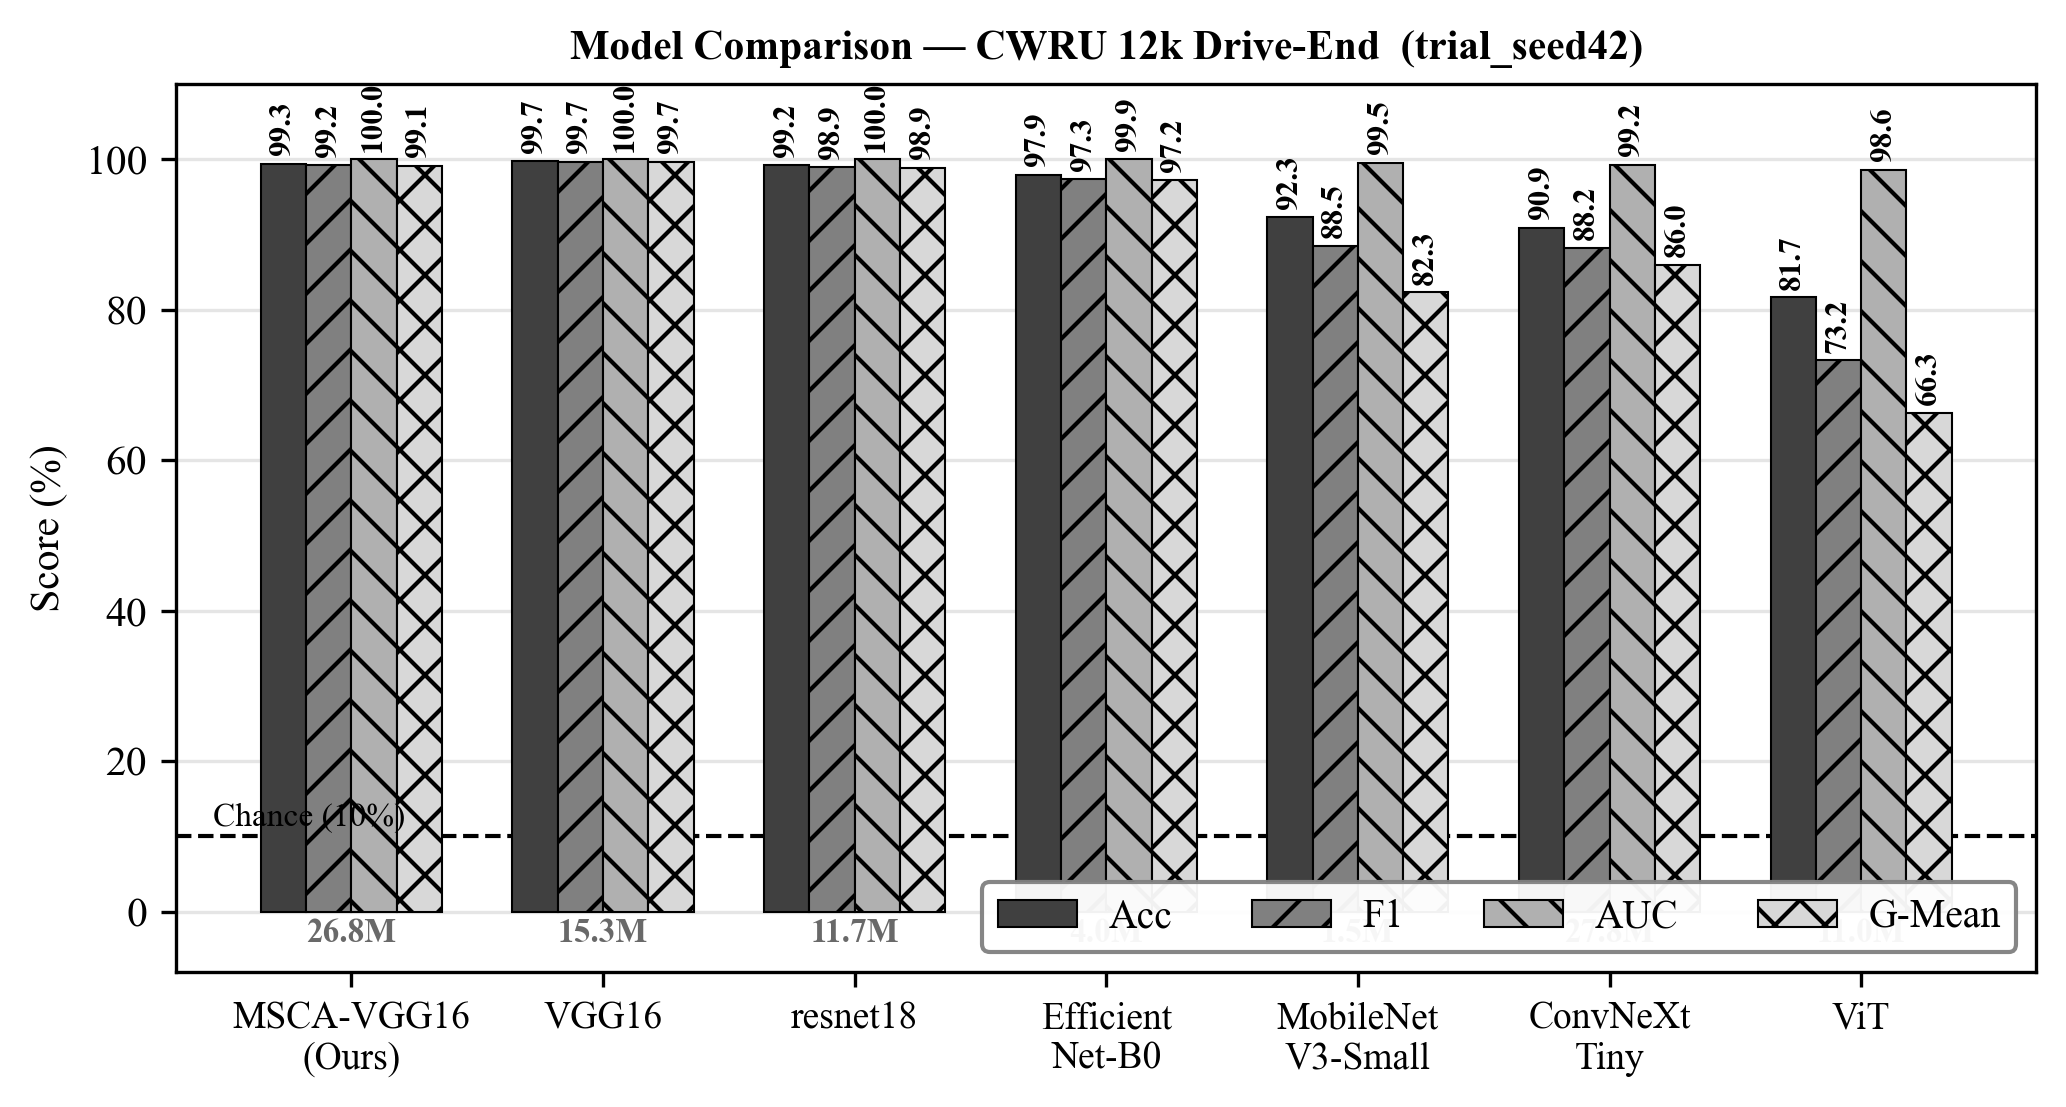
\includegraphics[width=\linewidth]{figures/model_comparison/model_comparison_12k_de_trial_seed42.png}
% \caption{}
% \label{}
% \end{figure*}


% The overall architecture of the proposed MSCA-VGG16 network is illustrated in Fig.~\ref{MSCA-VGG}.
% \begin{figure*}[!htbp]
% 	\centering
% 	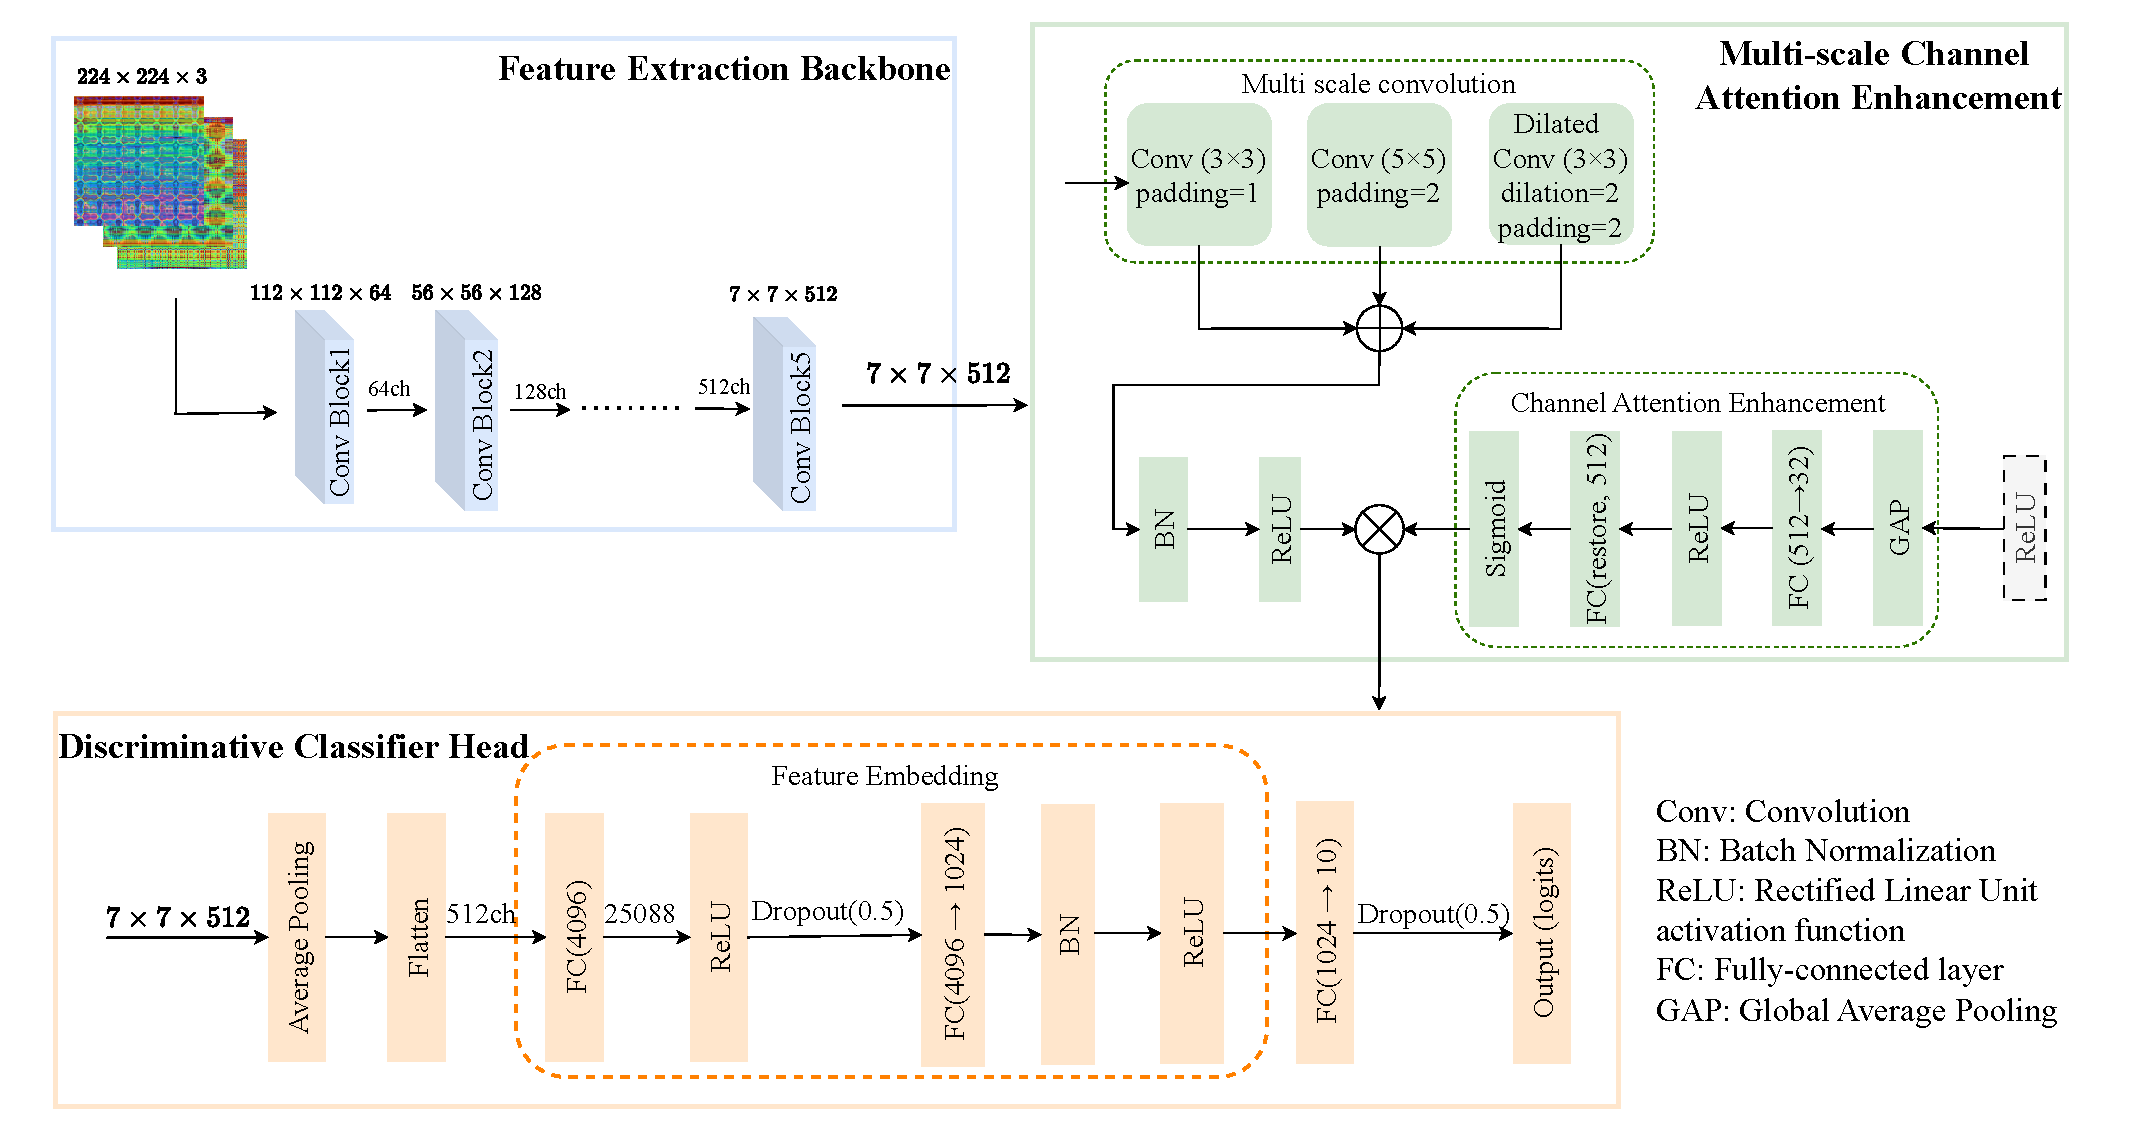
\includegraphics[width=\textwidth]{MSCA-VGG16/MSCA-VGG16}
% 	\caption{Overall architecture of the proposed MSCA-VGG16 network. The fused AW-DPCNN image is processed by a convolutional backbone, followed by a multi-scale convolution module, squeeze-and-excitation channel attention, and a compact embedding head for fault classification.}
% 	\label{MSCA-VGG}
% \end{figure*}


\bibliographystyle{IEEEtran}
\bibliography{references}

\end{document}